\documentclass[fontsize=12pt,paper=a4,twoside,bibtotoc,idxtotoc,
liststotoc,pagesize,BCOR1.2cm,DIV15,chapterprefix,pagesize=pdftex]{scrbook}

%\usepackage[utf8x]{inputenc}
\usepackage[ngerman]{babel}
\usepackage{amsmath}
\usepackage{amssymb}
\usepackage{dsfont}
\usepackage{textcomp}
\usepackage{stmaryrd}
\usepackage{graphicx}
\usepackage{xcolor}
\usepackage{tikz}
\usepackage[xetex,dvipdfmx]{animate}
\usepackage{mathtools}
\usepackage{amsthm}

\theoremstyle{plain}
\newtheorem{sz}[equation]{Satz}
\newtheorem{lm}[equation]{Lemma}
%\newtheorem{pf}{Beweis}
\theoremstyle{definition}
\newtheorem{df}[equation]{Definition}
\newtheorem{nt}[equation]{Notation}
\theoremstyle{remark}
\newtheorem{bem}[equation]{Bemerkung}

\title{Einführung in Sage}
\author{Dr.Jochen Schulz}
\date{10-10-11}


%\usepackage{fontspec,xunicode}
% %\usepackage{polyglossia}
%\setdefaultlanguage[spelling=new, latesthyphen=true]{german}
%\setsansfont{DejaVu Sans}
%\setsansfont{Verdana}
%\setsansfont{Arial}
%\setromanfont[Mapping=tex-text]{Linux Libertine}
%\setsansfont[Mapping=tex-text]{Myriad Pro}
%\setmonofont[Mapping=tex-text]{Courier New}

%\setsansfont{Linux Biolinum}

\usepackage[ngerman]{babel}
\selectlanguage{ngerman}

%
% math/symbols
%
\usepackage{amssymb}
\usepackage{amsthm}
% \usepackage{latexsym}
\usepackage{amsmath}
%\usepackage{amsxtra} %Weitere Extrasymbole
%\usepackage{empheq} %Gleichungen hervorheben
%\usepackage{bm}
 %\bm{A} Boldface im Mathemodus
\usepackage{fontspec,xunicode,xltxtra}

\usepackage{multimedia}
%\usepackage{tikz}

\usepackage{cellspace}
\setlength{\cellspacetoplimit}{2pt}
\setlength{\cellspacebottomlimit}{2pt}

%%%%%%%%%%%%%%%%%% Fuer Frames [fragile]-Option verwenden!
%Programm-Listing
%%%%%%%%%%%%%%%%%%
%Listingsumgebung fuer verbatim
%Grauhinterlegeter Text
%Automatischer Zeilenumbruch ist aktiviert
%\usepackage{listings}
\usepackage[framed]{mcode}
%\usepackage{mcode}
% This command allows you to typeset syntax highlighted Matlab
% code ``inline''.
% mcode fuer matlab

\definecolor{lgray}{gray}{0.80}
\definecolor{gray}{gray}{0.3}
\definecolor{darkgreen}{rgb}{0,0.4,0}
\definecolor{darkblue}{rgb}{0,0,0.8}
\definecolor{key}{rgb}{0,0.5,0} 
\definecolor{NU0}{RGB}{68,85,136} % #458
\definecolor{KW3}{RGB}{85,68,136}
\definecolor{KW4}{RGB}{153,0,0}
\definecolor{dred}{RGB}{221,17,68} % #d14
\definecolor{BG}{RGB}{240,240,240}
%\lstset{backgroundcolor=\color{lgray}, frame=single, basicstyle=\ttfamily, breaklines=true}
%\lstnewenvironment{sage}{\lstset{,language=python, keywordstyle=color{blue},    commentstyle=color{green}, emphstyle=\color{red}, %frame=single, stringstyle=\color{red}, basicstyle=\ttfamily, ,mathescape =true,escapechar=§}}{}

\lstdefinelanguage{fooHaskell} {%
  basicstyle=\footnotesize\ttfamily,%
  commentstyle=\slshape\color{gray},%
  keywordstyle=\bfseries,%\color{KW4},
  breaklines=true,
  sensitive=true,
  xleftmargin=1pc,
  emph={[1]
    FilePath,IOError,abs,acos,acosh,all,and,any,appendFile,approxRational,asTypeOf,asin,
    asinh,atan,atan2,atanh,basicIORun,break,catch,ceiling,chr,compare,concat,concatMap,
    const,cos,cosh,curry,cycle,decodeFloat,denominator,digitToInt,div,divMod,drop,
    dropWhile,either,elem,encodeFloat,enumFrom,enumFromThen,enumFromThenTo,enumFromTo,
    error,even,exp,exponent,fail,filter,flip,floatDigits,floatRadix,floatRange,floor,
    fmap,foldl,foldl1,foldr,foldr1,fromDouble,fromEnum,fromInt,fromInteger,fromIntegral,
    fromRational,fst,gcd,getChar,getContents,getLine,head,id,inRange,index,init,intToDigit,
    interact,ioError,isAlpha,isAlphaNum,isAscii,isControl,isDenormalized,isDigit,isHexDigit,
    isIEEE,isInfinite,isLower,isNaN,isNegativeZero,isOctDigit,isPrint,isSpace,isUpper,iterate,
    last,lcm,length,lex,lexDigits,lexLitChar,lines,log,logBase,lookup,map,mapM,mapM_,max,
    maxBound,maximum,maybe,min,minBound,minimum,mod,negate,not,notElem,null,numerator,odd,
    or,ord,otherwise,pi,pred,primExitWith,print,product,properFraction,putChar,putStr,putStrLn,quot,
    quotRem,range,rangeSize,read,readDec,readFile,readFloat,readHex,readIO,readInt,readList,readLitChar,
    readLn,readOct,readParen,readSigned,reads,readsPrec,realToFrac,recip,rem,repeat,replicate,return,
    reverse,round,scaleFloat,scanl,scanl1,scanr,scanr1,seq,sequence,sequence_,show,showChar,showInt,
    showList,showLitChar,showParen,showSigned,showString,shows,showsPrec,significand,signum,sin,
    sinh,snd,span,splitAt,sqrt,subtract,succ,sum,tail,take,takeWhile,tan,tanh,threadToIOResult,toEnum,
    toInt,toInteger,toLower,toRational,toUpper,truncate,uncurry,undefined,unlines,until,unwords,unzip,
    unzip3,userError,words,writeFile,zip,zip3,zipWith,zipWith3,listArray,doParse
  },%
  emphstyle={[1]\color{NU0}},%
  emph={[2]
    Bool,Char,Double,Either,Float,IO,Integer,Int,Maybe,Ordering,Rational,Ratio,ReadS,Show,ShowS,String,
    Word8,InPacket
  },%
  emphstyle={[2]\bfseries\color{KW4}},%
  emph={[3]
    case,class,data,deriving,do,else,if,import,in,infixl,infixr,instance,let,
    module,of,primitive,then,type,where
  },
  emphstyle={[3]\color{darkblue}},
  emph={[4]
    quot,rem,div,mod,elem,notElem,seq
  },
  emphstyle={[4]\color{NU0}\bfseries},
  emph={[5]
    EQ,False,GT,Just,LT,Left,Nothing,Right,True,Show,Eq,Ord,Num
  },
  emphstyle={[5]\color{KW4}\bfseries},
  morestring=[b]",%
  morestring=[b]',%
  stringstyle=\color{darkgreen},%
  showstringspaces=false
}
\lstnewenvironment{hs}
{\lstset{language=fooHaskell,backgroundcolor=\color{BG}}}
{\smallskip}
\newcommand{\ihs}[1]{\lstset{language=fooHaskell,basicstyle=\color[gray]{0.6}}\lstinline|#1|}


\lstdefinelanguage{fooMatlab} {%
backgroundcolor=\color[gray]{0.9},
breaklines=true,
basicstyle=\ttfamily\small,
%otherkeywords={ =},
%keywordstyle=\color{blue},
%stringstyle=\color{darkgreen},
showstringspaces=false,
%emph={for, while, if, elif, else, not, and, or, printf, break, continue, return, end, function},
%emphstyle=\color{blue},
%emph={[2]True, False, None, self, NaN, NULL},
%emphstyle=[2]\color{key},
%emph={[3]from, import, as},
%emphstyle=[3]\color{blue},
%upquote=true,
%morecomment=[s]{"""}{"""},
%commentstyle=\color{gray}\slshape,
%framexleftmargin=1mm, framextopmargin=1mm, 
%title=\tiny matlab,
frame=single,
%mathescape =true,
%escapechar=§
}
\newcommand{\imatlab}[1]{\lstset{language=fooMatlab,basicstyle=\color[gray]{0.6}}\lstinline|#1|}
\lstnewenvironment{matlab}[1][]{\lstset{language=fooMatlab,xleftmargin=0.2cm,frame=none,backgroundcolor=\color{white},basicstyle=\color{darkblue}\ttfamily\small,#1}}{} 
\lstnewenvironment{matlabin}[1][]{\lstset{language=fooMatlab,#1}}{} 
\newcommand{\matinput}[1]{\lstset{language=fooMatlab}\lstinputlisting{#1}}

\lstdefinelanguage{fooPython} {%
language=python,
backgroundcolor=\color[gray]{0.7},
breaklines=true,
basicstyle=\ttfamily\small,
%otherkeywords={ =},
keywordstyle=\color{blue},
stringstyle=\color{darkgreen},
morestring=[b]",%
morestring=[b]',%
showstringspaces=false,
emph={class, pass, in, for, while, if, is, elif, else, not, and, or,
def, print, exec, break, continue, return, import, from, lambda, null},
emphstyle=\color{blue},
emph={[2]True, False, None, self},
emphstyle=[2]\color{key},
emph={[3]from, import, as},
emphstyle=[3]\color{blue},
upquote=true,
morecomment=[s]{"""}{"""},
comment=[l]{\#},
commentstyle=\color{gray},
%framexleftmargin=1mm, framextopmargin=1mm, 
%title=\tiny python,
%caption=python,
frame=single
%frameround=tttt,
%mathescape =true,
%escapechar=§
}

\newcommand{\pyinput}[1]{\lstset{language=fooPython}\lstinputlisting{#1}}
\newcommand{\isage}[1]{{\lstset{language=fooPython,basicstyle=\color[gray]{0.3}}\lstinline|#1|}}

\lstnewenvironment{pyout}[1][]{\lstset{language=fooPython,xleftmargin=0.2cm,frame=none,backgroundcolor=\color{white},basicstyle=\color{darkblue}\ttfamily\small,#1}}{}
\lstnewenvironment{pyin}[1][]{\lstset{language=fooPython,#1}}{}
\lstnewenvironment{sageout}[1][]{\lstset{language=fooPython,xleftmargin=0.2cm,frame=none,backgroundcolor=\color{white},basicstyle=\color{darkblue}\ttfamily\small,#1}}{}
\lstnewenvironment{sagein}[1][]{\lstset{language=fooPython,#1}}{}

%\usepackage{caption}
%\DeclareCaptionFont{white}{ \color{white} }
%\DeclareCaptionFormat{listing}{
%  \colorbox[cmyk]{0.43, 0.35, 0.35,0.01 }{
%      \parbox{\textwidth}{\hspace{15pt}#1#2#3}
%        }
%        }
%        \captionsetup[lstlisting]{ format=listing, labelfont=white, textfont=white, singlelinecheck=false, margin=0pt, font={bf,footnotesize} }


\usepackage{mydef}
%\usepackage{cmap} % you can search in the pdf for umlauts and ligatures
\usepackage{colonequals} %corrects the definition-symbols \colonequals (besides others)

\usepackage{ifthen}

%%%%%%%%%%%%%%%%%%%
%Neue Definitionen
%%%%%%%%%%%%%%%%%%%

%Newcommands
\newcommand{\Fun}[1]{\mathcal{#1}}      %Mathcal fuer Funktoren
\newcommand{\field}[1]{\mathbb{#1}}     %Grundkoerper ?? in mathds

\newcommand{\A}{\field{A}}              %Affines A
\newcommand{\Fp}{\field{F}_{\!p}}       %Endlicher Koerper mit p Elementen
\newcommand{\Fq}{\field{F}_{\!q}}       %Endlicher Koerper mit q Elementen
\newcommand{\Ga}{\field{G}_{a}}         %Add Gruppenschema
\newcommand{\K}{\field{K}}              %Generischer Koerper 
\newcommand{\N}{\field{N}}              %Nat Zahlen
\newcommand{\Pj}{\field{P}}             %Projektives P
\newcommand{\R}{\field{R}} 		%Reelle Zahlen
\newcommand{\Q}{\field{Q}}              %Rationale Zahlen  
\newcommand{\Qt}{\field{H}}             %Quaternionen 
\newcommand{\V}{\field{V}}              %Vektorbuendel V
\newcommand{\Z}{\field{Z}}              %Ganze Zahlen
\DeclareMathOperator{\Real}{Re}

\newcommand{\fdg}{\;|\;}                 %fuer die gilt

%Operatoren
\DeclareMathOperator{\Abb}{Abb}
%\usepackage{sagetex}


%
% Aufgaben
%
\parindent0cm % Abs�tze nicht einr�cken 
% Definieren einer neuen Farbe
\definecolor{light-gray}{gray}{.9}

\newcounter{zaehler}     % neuen Z�hler einf�hren
\newenvironment{aufgn}[2][0]
%---- Header
{\begin{samepage}%
%\colorbox{light-gray}{%                         % Box in gray
% \makebox[\textwidth]{%                           % Box in linewidth
%\textbf{Aufgabe \arabic{zaehler} } }\hspace{-\textwidth}\makebox[\textwidth]{\hfill #1 Punkte} }\\[0.05cm]       % Header
\dotfill\\
{\large\textbf{Aufgabe \arabic{zaehler} \ifthenelse{ \equal{#2}{} }{}{: \emph{ #2 } }}\ifthenelse{-1=#1}{(testierbar)}{}\ifthenelse{0=#1 \or -1=#1}{}{\hfill #1 Punkte} }\\[0.4cm]
%{\large\textbf{Exercise \arabic{zaehler}  #2 }\ifthenelse{-1=#1}{(testierbar)}{}\ifthenelse{0=#1 \or -1=#1}{}{\hfill #1 Punkte} }\\[0.4cm]
\begin{minipage}{\textwidth}%
}%
%-----  foot
{\end{minipage}\nopagebreak%\begin{minipage}{1cm} \end{minipage}
%\\ 
%\begin{minipage}{0.1cm} \end{minipage} 
%\hrulefill \begin{minipage}{1cm} \end{minipage}\\[1cm]  
\stepcounter{zaehler}                           % increase counter
\end{samepage}%
\\%
\bigskip%
}


\newenvironment{aufg}[1][0]
%---- Header
{\begin{samepage}%
\refstepcounter{zaehler}% increase counter
%\colorbox{light-gray}{%                         % Box in gray
% \makebox[\textwidth]{%                           % Box in linewidth
%\textbf{Aufgabe \arabic{zaehler} } }\hspace{-\textwidth}\makebox[\textwidth]{\hfill #1 Punkte} }\\[0.05cm]       % Header
\dotfill\\
{\large\textbf{Aufgabe \arabic{zaehler} }\ifthenelse{-1=#1}{(testierbar)}{}\ifthenelse{0=#1 \or -1=#1}{}{\hfill #1 Punkte} }\\[0.4cm]
\begin{minipage}{\textwidth}%
}%
%-----  foot
{\end{minipage}\nopagebreak%\begin{minipage}{1cm} \end{minipage}
%\\ 
%\begin{minipage}{0.1cm} \end{minipage} 
%\hrulefill \begin{minipage}{1cm} \end{minipage}\\[1cm]  
\end{samepage}%
\\%
\bigskip%
}

\begin{document}
\maketitle
\tableofcontents
%%%%%%%%%%%%%%%%%%%%%%%%%%%%%%%%%%%%%%
\chapter{Sage Überblick}
\section{Was ist Sage?}
%\subsection{Was ist Sage?}
%%%%%%%%%%%%%%%%%%%%%%%%%%%%%%%%%%%%%%
Sage ist ein pythonbasiertes, objektorientiertes Open-source (GPL) Mathematik Software System, dass es seit dem 24. Februar 2005 gibt.
In Sage findet man eine Alternative zu den 4 M's: Magma, Maple, Mathematica, Matlab.
Das (Haupt-)Interface ist der Browser, dennoch besitzt Sage Frontends für viele externe Software.
Zu den Stärken von Sage zählt sicherlich, dass es viele andere CAS und Libraries unter einer einheitlichen Oberfläche vereint 
(so z.B. Maxima, Pari, GAP, R, Magma, ...), sowie durch Python eine sehr mächtige Programmiersprache als Grundlage hat. Desweiteren 
ist der Source Code offen, es gibt ein umfangreiches Hilfesystem sowie viele freie Materialien im Internet.
Wie alles, so hat auch Sage trotz seiner vielen Stärken auch Schwächen, so ist der Befehlsumfang nicht so mächtig, wie der von Maple,Mathematica 
oder Matlab; außerdem fehlt eine standalone Entwicklungsumgebung. Als Alternative zum Webinterface findet sich Cantor.
%%%%%%%%%%%%%%%%%%%%%%%%%%%%%%%%%%%%%%
\subsection{Grundlegende Commandos}
%%%%%%%%%%%%%%%%%%%%%%%%%%%%%%%%%%%%%%
Sage incl. online Testversion und gratis Download sowie einigen anderen Features findet sich unter http://www.sagemath.org/.
Hier ein paar grundlegende Tipps, Tricks und Dinge, die einfach beherzigt werden sollten:
\begin{itemize}
 \item Mehrere Befehle in einer Zeile durch {\color{blue} \verb~;~} trennen. 
 \item Bei Eingaben, die über mehrere Zeilen gehen, kann ein
  Zeilenumbruch durch {\color{blue} \verb~<ENTER>~} erreicht werden.
 \item Das Auswerten eines Blocks erfolgt mit {\color{blue} \verb~<SHIFT>+<ENTER>~}.
 \item Ein neues Eingabefeld erhält man durch klicken auf den blauen, horizontalen Balken
 \item {\color{blue} \isage{_} } refenziert die letzte Ausgabe.
 \item Löschen aller eigenen Variablen und Zurücksetzen auf den Anfangsstatus: {\color{blue} \isage{reset()}}
% Anzeigen aller definierten Variablen: {\color{blue} anames(All)}
% Anzeigen aller selbst definierten Variablen: {\color{blue} anames(All,User)}
 \item Das Feld aktivieren von \emph{Typeset} lässt alle Ausgaben von \LaTeX{} rendern.
% profiler und debugger -> commandline
 \item Html- und/oder \LaTeX-Dokumentation:{\color{blue} \verb~<SHIFT>+<KLICK>~ }auf den blauen Balken
% Publish: Im Notebook kann durch klicken des \alert{Publish}-Reiters das Notebook für alle offen gelegt werden. 
% Unter dem Menupunkt \alert{File} kann man 
 \item {\color{blue} Autocompletion :} mit der {\color{blue} \verb~<TAB>~}-Taste erhält man alle möglichen Funktions- und Variablen-Namen im gegebenen Kontext.\\
  Dies gilt insbesondere auch für Objektfunktionen (\isage{object.function()})
  \item{\color{blue} \isage{<command>?} :} gibt ausführliche Hilfe zu \isage{command} an.
 \item {\color{blue} \isage{help(<command>)} :} öffnet ein Hilfefenster zu \isage{command}.
 \item online Dokumentation:
    \begin{itemize}
    \item Sage: http://www.sagemath.org/doc/index.html
    \item Python: http://docs.python.org/
    \end{itemize}
\end{itemize}  
%%%%%%%%%%%%%%%%%%%%%%%%%%%%%%%%%%%%%%
\section{Überblick über wichtige Operationen}
%%%%%%%%%%%%%%%%%%%%%%%%%%%%%%%%%%%%%%
Als Einstieg und kleine Motivation, wofür man Sage einsetzen kann, wollen wir erst einmal ein paar grundlegende Operationen 
vorstellen:
\begin{itemize}
 \item Deklarieren von Variablen mit \isage{var()}, z.B.{\verb~var('a')~} 
 \item Definieren von Variablen mit {\color{blue}'='}, z.B. {\verb~a=3~} 
 \item Definieren von Funktionen mit{\color{blue} '='}, z.B. {\verb~f(x) = x^2 - 6*x~}
 \item Grenzwertbestimmung: {\color{blue}   \verb~f.limit(x=1, dir='<plus|minus>')~}
 \item Bilden von Ableitungen: {\color{blue} \verb~f.differentiate(x)~}
 \item Lösen von Gleichungen: {\color{blue} \verb~solve( f(x)==0, x)~}
 \item Berechnen numerischer Approximationen: {\color{blue} \verb~float(f(sqrt(3)+ 4))~}
 \item Plotten einer Funktion: {\color{blue} \verb~plot(sin,(0,4))~}
 \item symbolisch Integrieren: {\color{blue} \verb~integrate(f,x)~}
 \item numerisch Integrieren: {\color{blue} \verb~integrate(f,x,a,b)~}
 \item Faktorisieren: {\color{blue} \verb~expand(f)~}
 \item Sortieren: {\color{blue} \verb~f.collect(x)~}
 \item Partialbruchzerlegung: {\color{blue} \verb~f.partial_fraction()~}
 \item vollständiges Vereinfachen: {\color{blue} \verb~f.full_simplify()~}
 \item Vereinfachen mit radicals: {\color{blue} \verb~f.radical_simplify()~}
 \item Matrix eingeben: {\color{blue} \verb~matrix([ [z1s1,z1s2],[z2s1,z2s2] ])~}
 \item Vektor eingeben: {\color{blue} \verb~vector([a,b,c])~}
 \item LGS lösen: {\color{blue} \verb~A\b~}
 \item Matrixoperationen: {\color{blue} \verb~A+B,A-B,A*B~}
 \item Matrix invertieren: {\color{blue} \verb~A^(-1); A.inverse()~}
 \item Substitutieren: {\color{blue} \verb~f.subs(k=2)~}
\end{itemize}
Hiermit stehen uns nun einige Türen offen und wir wollen uns durch ein paar Beispiele der Sagewelt nähern:
%%%%%%%%%%%%%%%%%%%%%%%%%%%%%%%%%%%%%%
\subsection{Kurvendiskussion}
%%%%%%%%%%%%%%%%%%%%%%%%%%%%%%%%%%%%%%
Wir wollen eine handelsübliche Kurvendiskussion führen. Dazu betrachten wir die durch die reelle Zahl $a$ parametrisierte 
Funktionenschar:
\[ 
f: x \quad \mapsto \quad \frac{2x^2-20x+42}{x-1}+a, \quad
a \in \mathbb{R} 
\]
Wie bekommen wir nun diese Aufgabe mittels Sage gelöst? Zuerst sollten wir diese Funktionenschar wohl Sage ``erklären'', 
um weiter mit ihr arbeiten zu können. Dies geschieht, indem wir zuerst die Variable $a$ und anschließend die Funktion selbst 
deklarieren:
\begin{sagein}
var('a')
f(x) = (2*x^2-20*x +42)/(x-1)+a;f
\end{sagein}
\begin{bem} Die Multiplikationszeichen dürfen NICHT weggelassen werden.\end{bem}
Wir erhalten als Antwort
\begin{sage}
  x |--> a + 2*(x^2 - 10*x + 21)/(x - 1)
\end{sage}
\begin{bem} Es findet keine Ausgabe statt, wenn wir in unserer Eingabe ;f weglassen.\end{bem}
Wir möchten nun herausfinden, ob unsere Funktion $f$ Polstellen besitzt; dazu benutzen wir den {\color{blue} \verb limit() }-Befehl:
\begin{sagein}
f.limit(x=1, dir='minus')
\end{sagein}
\begin{sage}
  x |--> -Infinity
\end{sage}
\begin{sagein}
f.limit(x=1, dir='plus') 
\end{sagein}
\begin{sage}
  x |--> +Infinity
\end{sage}
Wir sehen nun, dass unsere Funktion $f$ an der Stelle x=1 einen Pol hat. Wir verfahren weiter mit der Suche nach Nullstellen 
und wenden dafür den {\color{blue} \verb solve() }-Befehl an:
\begin{sagein}
solve(f==0,x)
\end{sagein}
\begin{sage}
[x == -1/4*a - 1/4*sqrt(a^2 - 32*a + 64) + 5, x == -1/4*a + 1/4*sqrt(a^2 - 32*a + 64) + 5]
\end{sage}
Wir haben nun 2 Nullstellen gefunden und stellen uns sogleich die Frage nach der Ableitung von $f$, die wir über den 
{\color{blue} \verb differentiate() }-Befehl erhalten:
\begin{sagein}
f.differentiate(x)
\end{sagein}
\begin{sage} 
x |--> 4*(x - 5)/(x - 1) - 2*(x^2 - 10*x + 21)/(x - 1)^2
\end{sage}
Da unsere Funktion $f$ offenbar eine Ableitung besitzt, interessiert uns, ob und, wenn ja, wo $f$ Extrema besitzt sowie die Antwort 
auf die Frage, ob es sich um Minima oder Maxima handelt:
\begin{sagein}
maxi = solve(f.differentiate(x)==0,x); maxi
\end{sagein}
\begin{sage}
[x == -2*sqrt(3) + 1, x == 2*sqrt(3) + 1]
\end{sage}
\begin{sagein}
float( ((f.diff(x)).diff(x))(maxi[0].rhs()) )
\end{sagein}
\begin{sage}
-1.1547005383792501
\end{sage}
\begin{sagein}
float( ((f.diff(x)).diff(x))(maxi[1].rhs()) )
\end{sagein}
\begin{sage}
1.1547005383792515
\end{sage}
Wir erkennen die Existenz zweier Extremstellen, von denen eine ein Maximum, die andere ein Minimum ist.
\begin{bem} Als ``Speicherplatz'' der Nullstellen von $f'$ besitzt maxi zwei Werte-- diese werden mit maxi[0].rhs() 
bzw maxi[1].rhs() angesprochen.\end{bem}
Ohne den {\color{blue} \verb float() }-Befehl sähe die Ausgabe im ersten Fall so aus:
\begin{sagein}
-1/18*((2*sqrt(3) - 1)^2 + 20*sqrt(3) + 11)*sqrt(3) + 2/3*sqrt(3) + 8/3
\end{sagein}
und wäre somit unbrauchbar, um direkt ein Maximum oder Minimum erkennen zu können.
Zuletzt betrachten wir noch das Verhalten am Rande:
\begin{sagein}
f.limit(x=oo); f.limit(x=-oo)
\end{sagein}
\begin{sage}
x |--> +Infinity
x |--> -Infinity
\end{sage}
\begin{bem} Wir erkennen, in Sage stellt sich $\infty$ dar via oo, $-\infty$ entspricht -oo.
Viel interessanter jedoch ist die Tatsache, dass Sage mit jenen ``Werten'' direkt arbeiten zu können scheint.\end{bem}
Zuletzt wollen wir uns mit der grafischen Darstellung einiger Repräsentanten von f auseinandersetzen. Hierzu wollen wir zuerst 3 
jener Repräsentanten deklarieren und diese anschließend mit dem {\color{blue} \verb plot() }-Befehl visualisieren:
\begin{sagein}
 f0 = f(x, a=0)
 f1 = f(x, a=-20)
 f2 = f(x, a=20);f0,f1,f2
\end{sagein}
\begin{sage}
(2*(x^2 - 10*x + 21)/(x - 1), 2*(x^2 - 10*x + 21)/(x - 1) - 20, 2*(x^2 - 10*x + 21)/(x - 1) + 20)
\end{sage}
\begin{sagein}
p = plot(f0,detect_poles='show',xmin=0, xmax=10,color='red')
p += plot(f1,detect_poles='show',xmin=0, xmax=10,color='green')
p += plot(f2,detect_poles='show',xmin=0, xmax=10,color='blue'); p.show(ymin=-80, ymax=80)
\end{sagein}
Wir erhalten als Grafikausgabe:
\begin{center}
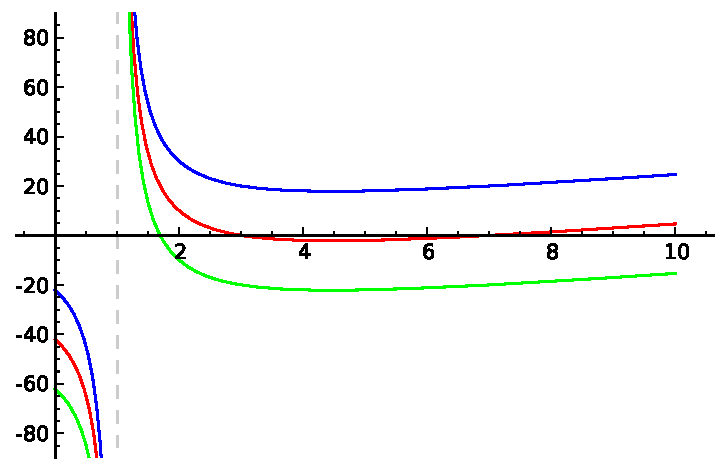
\includegraphics[height=4.5cm]{graphen}
\end{center}
%%%%%%%%%%%%%%%%%%%%%%%%%%%%%%%%%%%%%%
\subsection{Symbolisches Rechnen}
%%%%%%%%%%%%%%%%%%%%%%%%%%%%%%%%%%%%%%
Wir wollen uns nun ein wenig mit symbolischem Rechnen vertraut machen. Dazu zählt das numerische Lösen von Integralen, 
sicherlich aber auch die Vereinfachung oder die Faktorisierung eines Terms. 
Wir betrachten einige Beispiele:
Wir möchten gerne das Integral $\int_0^\infty x^4 e^{-x} dx$ numerisch berechnen, dazu benötigen wir lediglich
\begin{sagein}
integrate(x^4*exp(-x),x,0,oo)
\end{sagein}
und erhalten als Ausgabe 
\begin{sage}
  24
\end{sage}
Wollen wir eine Stammfunktion von $\frac{1+\sin (x)}{1+\cos(x)}$ berechnen, so genügt uns die Deklaration zweier Funktion f
und g wie folgt:
\begin{sagein}
f(x) = (1+sin(x))/(1+cos(x))
g = f.integrate(x);g
\end{sagein}
\begin{sage}
x |--> sin(x)/(cos(x) + 1) - log(cos(x) + 1)
\end{sage}
Die Funktion g sieht eher unschön aus, wir möchten sie daher vereinfachen und benutzen dafür
\begin{sagein}
g.full_simplify()
\end{sagein}
\begin{sage}
x |--> -((cos(x) + 1)*log(cos(x) + 1) - sin(x))/(cos(x) + 1)
\end{sage}
Die Verschönerung hat hier nur bedingt geklappt, aber der Versuch war es wert und oft erhält man wirklich ein schöneres 
Ergebnis als zuvor. Ein wenig effektiver funktioniert es mit ($\frac{e^x -1}{e^{(1/2)x}+1}$)
\begin{sagein}
g = (exp(x)-1)/(exp(x/2)+1)
g.simplify_radical()
\end{sagein}
\begin{sage}
 e^(1/2*x) - 1
\end{sage}
Es gibt noch andere Möglichkeiten, Termen ein schöneres Aussehen zu geben. Betrachten wir den Term
\begin{sage}
x^4 - 10*x^3 + 35*x^2 - 50*x + 24
\end{sage}
und fragen uns: Können wir ihn Faktorisieren? Eine Antwort darauf liefert 
\begin{sagein}
factor(x^4 - 10*x^3 + 35*x^2 - 50*x + 24)
\end{sagein}
\begin{sage}
(x - 4)*(x - 3)*(x - 2)*(x - 1)
\end{sage}
Als kleine Probe können wir die Faktorisierung rückgängig machen:
\begin{sagein}
expand(_)
\end{sagein}
\begin{sage}
x^4 - 10*x^3 + 35*x^2 - 50*x + 24
\end{sage}
\begin{bem} Wir erinnern uns, dass {\color{blue} \verb _ } eine Referenz auf die letzte Ausgabe ist.\end{bem}
Wir können Terme auch bzgl. einer Variablen sortieren:
\begin{sagein}
var('b,a')
g = x^2+2*x+b*x^2+sin(x)+a*x
g.collect(x)
\end{sagein}
\begin{sage}
(b + 1)*x^2 + (a + 2)*x + sin(x)
\end{sage}
Zuletzt steht uns hier noch die Partialbruchzerlegung zur Verfügung:
\begin{sagein}
g = x^ 2/( x^ 2- 1)
g.partial_fraction()
\end{sagein}
\begin{sage}
1/2/(x - 1) - 1/2/(x + 1) + 1
\end{sage}
%%%%%%%%%%%%%%%%%%%%%%%%%%%%%%%%%%%%%%
\subsection{Analytische Geometrie und Lineare Algebra}
%%%%%%%%%%%%%%%%%%%%%%%%%%%%%%%%%%%%%%
Wir wollen uns ein wenig mit analytischer Geometrie und linearer Algebra beschäftigen und zu Anfang mal den Schnittpunkt einer Ebene mit einer Geraden 
berechnen. Dazu sei die Ebene E gegeben durch
\[ E: \vec{x}= 
\left ( \begin{array}{c}  2 \\ 1 \\ -1 \end{array} \right) +l 
\left ( \begin{array}{c}  1 \\ -1 \\ -1 \end{array} \right) +m
\left ( \begin{array}{c}  -3 \\ 1 \\ 4 \end{array} \right), \quad l,m
\in \mathbb{R}
\]
und die Gerade g
\[
g: \vec{x}=
\left ( \begin{array}{c}  3 \\ 0 \\ 1 \end{array} \right) +k
\left ( \begin{array}{c}  4 \\ -1 \\ 2 \end{array} \right), \quad k \in \mathbb{R}
\]
Gleichsetzen ergibt: 
\[ 
\left ( \begin{array}{c}  2 \\ 1 \\ -1 \end{array} \right) +l 
\left ( \begin{array}{c}  1 \\ -1 \\ -1 \end{array} \right) +m
\left ( \begin{array}{c}  -3 \\ 1 \\ 4 \end{array} \right) = \left ( \begin{array}{c}  3 \\ 0 \\ 1 \end{array} \right) +k
\left ( \begin{array}{c}  4 \\ -1 \\ 2 \end{array} \right)
\] oder {
\[ 
\underbrace{\left(   
\begin{array} {ccc} 
1 & -3 & -4\\
-1 & 1 & 1 \\
-1 & 4 & -2  
\end{array} \right)}_{\displaystyle =:A} 
\underbrace{\left ( \begin{array}{c}  l \\ m \\ k \end{array}
  \right)}_{\displaystyle =:L} = \underbrace{\left ( \begin{array}{c}  1 \\ -1 \\ 2
  \end{array} \right)}_{\displaystyle =:b}
\] }
oder $A L=b$.
Wir wollen nun lineare Gleichungssysteme (wie dieses) wie gewöhnlich durch Matrizen beschreiben und via Sage lösen. Dazu benötigen wir ein paar Grundlagen:
 Definieren der Matrix $A$
\begin{sagein}
A = matrix([[1,-3,-4],[-1,1,1],[-1,4,-2]]); A
\end{sagein}
\begin{sage}
[ 1 -3 -4]
[-1  1  1]
[-1  4 -2]
\end{sage}
 Definieren des Vektors $b$
\begin{sagein}
b = vector([1,-1,2]);b
\end{sagein}
\begin{sage}
(1,-1,2) 
\end{sage}
 Lösen von  $A \ L=b$
\begin{sagein}
A.solve_right(b)
\end{sagein}
oder 
\begin{sagein}
A\b
\end{sagein}
ergibt
\begin{sage}
(6/5, 3/5, -2/5)
\end{sage}
 Einsetzen in die Geradengleichung
\begin{sagein}
x_s = matrix([g1,g2,g3]).subs(k=L[2]); x_s
\end{sagein}
\begin{sage}
[7/5 2/5 1/5]
\end{sage}
So haben wir nun recht aufwandsarm den Schnittpunkt der beiden Objekte E und g erhalten. Wir geben noch einen kurzen Ausblick auf weitere 
Matrizenoperationen:
\begin{sagein}
B = matrix([[1,0,0],[0,1,1],[1,1,1]])
A*B, A-B, A+B
\end{sagein}
\begin{sage}
(
[-3 -7 -7]   [ 0 -3 -4]  [ 2 -3 -4]
[ 0  2  2]   [-1  0  0]  [-1  2  2]
[-3  2  2],  [-2  3 -3], [ 0  5 -1]
)
\end{sage}
Berechnen der Inversen (mit Probe)
\begin{sagein}
$A^{(-1)}$, A*A^(-1)
\end{sagein}
\begin{sage}
(
[  -2/5 -22/15   1/15]  [1 0 0]
[  -1/5   -2/5    1/5]  [0 1 0]
[  -1/5  -1/15  -2/15], [0 0 1]
)
\end{sage}
Wir wollen uns das Ganze mal visualisieren, hierzu bietet uns Sage den 3D plot:
\begin{sagein}
var('l,m'); E1 = 2+l-3*m; E2 = 1-l+m; E3 =-1-l+4*m
p = parametric_plot3d([E1,E2,E3],(l,-2,2),(m,-2,2), color='green', opacity=0.8)
var('k'); g1 = 3+4*k; g2 = -k; g3 = 1+2*k
p += parametric_plot3d( (g1,g2,g3), (k, -3, 3),thickness='3' ) 
p.show()
\end{sagein}
\begin{center}
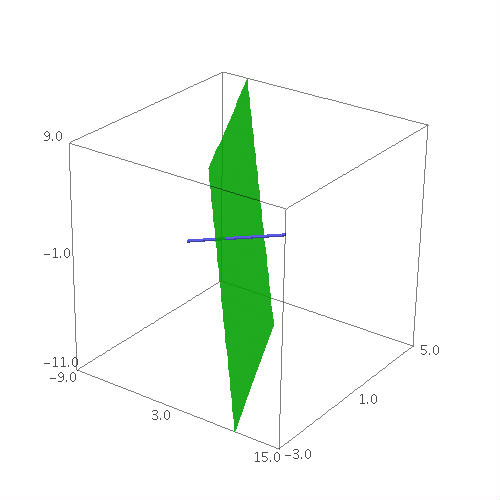
\includegraphics[width=0.7\textwidth]{ebene2}
\end{center}
\begin{bem} In Sage lässt sich der 3D plot drehen.\end{bem}
%%%%%%%%%%%%%%%%%%%%%%%%%%%%%%%%%%%%%%
\subsection{Programmieren}
%%%%%%%%%%%%%%%%%%%%%%%%%%%%%%%%%%%%%%
Sage erlaubt uns, eigene Funktionen von nahezu beliebigem Komplexitätsgrad zu schrieben. Wir wollen uns hier die einzeiligen Funktionen zusammen 
mit Listen und Tupeln sowie Schleifen anschauen-- um im Anschluss etwas Zahlentheorie zu betreiben. Beginnen wir mit den einzeiligen Funktionen, die 
wie folgt aufgebaut sind:
  \begin{sagein}
  def <name>(<Argumente>) : return <Rueckgabe>
  \end{sagein}
Um zu sehen, wie eine solche selbstdefinierte Funktion aussehen könnte, schreiben wir eine Funktion $fd(ex)$, die die Ableitung von $ex$ berechnet 
und sich der Einfachheit halber der sage-internen Funktion {\color{blue} \verb diff() } bedient:
  \begin{sagein}
  def fd(ex) : return diff(ex)
  fd(x^2)
  \end{sagein}
  \begin{sage}
  2*x
  \end{sage}
Sage kennt Listen und Tupel, in denen wir Objekte ablegen, zusammenfassen und noch einiges mehr können. Eine {\color{blue} \verb Liste } 
ist in Sage (und Python) durch \isage{[..,..]}, ein {\color{blue} \verb Tuple } durch \isage{(..,..)} gekennzeichnet. Wir haben einige 
interessante Operationen speziell für Listen:
  \begin{sagein}
  liste = [21,22,24,23]
  liste.sort(); liste 
  \end{sagein}
  \begin{sage}
  [21, 22, 23, 24]
  \end{sage}
\begin{bem}
 Wir erinnern uns, dass durch die {\color{blue} \verb~<TAB>~}-Taste eine Autovervollständigung verfügbar ist. Wenden wir sie auf die Eingabe
{\color{blue} \verb list. } an, erhalten wir eine Auflistung möglicher Operationen auf Listen.
\end{bem}
Fast analog haben wir Tuple:
  \begin{sagein}
  tuple = (liste[0], liste[2])
  tuple, tuple[0]
  \end{sagein}
  \begin{sage}
  ((21, 24), 21) 
  \end{sage}
\begin{bem}
 {\color{blue} \verb liste[i] } liefert das $i$-te Element der Liste liste.
\end{bem}
Wir werden oft eine Liste ganzer Zahlen von \isage{a} bis \isage{b} brauchen, sie von Hand zu erstellen wäre zwar möglich, doch Sage kommt uns 
gern durch sogar 2 Befehle entgegen:
  \begin{sagein}
  [a..b] ; range(a,b+1)
  \end{sagein}
Wir erstellen uns probehalber eine Liste der Zahlen von 1 bis 10:
\begin{sagein}
 a = [1..10];a
\end{sagein}
\begin{sage}
 [1, 2, 3, 4, 5, 6, 7, 8, 9, 10]
\end{sage}
Schauen wir uns nun etwas wirklich nützliches an: Schleifen! Wir unterscheiden grundlegend bedingte und unbedingte Schleifen:
  \begin{sagein}
  [<expr(var)> for <var> in <range|liste>] 
  [<expr(var)> for <var> in <range|liste> if <expr>] 
  \end{sagein}
Als kleine Aufwärmübung wollen wir uns die Quadrate der Zahlen von 1 bis 5 berechnen:
  \begin{sagein}
  [m^2 for m in [1..5] ]
  \end{sagein}
  \begin{sage}
  [1, 4, 9, 16, 25]
  \end{sage}
Und anschließend die Quadrate der Zahlen von 1 bis 5, die durch 2 teilbar sind:
  \begin{sagein}
  [m^2 for m in [1..5] if m%2==0]
  \end{sagein}
  \begin{sage}
  [4, 16]
  \end{sage}
%%%%%%%%%%%%%%%%%%%%%%%%%%%%%%%%%%%%%%
\subsection{Zahlentheorie}
%%%%%%%%%%%%%%%%%%%%%%%%%%%%%%%%%%%%%%
Wir sind nun in der Lage, etwas kompliziertere Aufgabenstellungen zu bearbeiten:
Die Fermatschen Primzahlen sind gegeben durch $F_n=2^{2^n} +1$. Wir wollen die kleinste dieser Zahlen finden, die keine Primzahl ist. Dazu 
schreiben wir uns ein kleines Programm:
\begin{sagein}
def F(n): return 2^(2^n)+1
[[F(m),is_prime(F(m))] for m in range(1,6)]
\end{sagein}
\begin{sage}
[[5, True], [17, True], [257, True], [65537, True], [4294967297, False]]
\end{sage}
Da $F_5$ keine Primzahl ist, interssieren uns nun noch die Teiler von $F_5$
\begin{sagein}
divisors(int(F(5)))
\end{sagein}
\begin{sage}
[1, 641, 6700417, 4294967297]
\end{sage}
 Wir möchten eine Liste der Primzahlen bis 100 und lösen unser Problem durch eine Schleife:
\begin{sagein}
menge = range(1,101)
[m for m in menge if is_prime(m)]
\end{sagein}
\begin{sage}
[2, 3, 5, 7, 11, 13, 17, 19, 23, 29, 31, 37, 41, 43, 47, 53, 59, 61, 67, 71, 73, 79, 83, 89, 97]
\end{sage}
 Sage hätte alternativ die {\color{blue} \verb filter() } Funktion geliefert, die allgemeiner nach (fast) beliebigen Merkmalen filtert:
\begin{sagein}
 filter(is_prime,menge)
\end{sagein}
 Die Mersenne Primzahlen sind gegeben durch $2^p-1$, dabei $p$ Primzahl. Wir wollen die Mersenne Primzahlen im Bereich $\leq200$ bestimmen:
\begin{sagein}
menge = range(1,201)
primes = [m for m in menge if is_prime(m)]
[2^m-1 for m in primes if is_prime(2^m-1)]
\end{sagein}
\begin{sage}
[3, 7, 31, 127, 8191, 131071, 524287, 2147483647, 2305843009213693951,
618970019642690137449562111, 162259276829213363391578010288127,
170141183460469231731687303715884105727]
\end{sage}
Wir widmen uns einer etwas komplizierteren Aufgabe: Wir wollen für die Zahlen $\leq1000$ bestimmen, wieviele Zahlen 1,2,3,... Teiler haben:
\begin{sagein}
menge = range(1,1001)
liste = [number_of_divisors(int(m)) for m in menge]
[(i,len([m for m in liste if m==i]))for i in range(1,51)]
\end{sagein}

\begin{sage}
[(1, 1), (2, 168), (3, 11), (4, 292), (5, 3), (6, 110), (7, 2), (8,
180), (9, 8), (10, 22), (11, 0), (12, 97), (13, 0), (14, 5), (15, 4),
...
\end{sage}
Bis hierher haben wir einen kleinen Rundumblick genommen, einige sehr elementare Grundlagen kennengelernt und sind schon recht vertraut mit 
Sage. Vieles von dem, was wir bisher gesehen haben, wird uns wieder begegnen, wenn wir uns weiter mit Sage befassen.
%%%%%%%%%%%%%%%%%%%%%%%%%%%%%%%%%%%%%%
\chapter{Grundlagen}
%%%%%%%%%%%%%%%%%%%%%%%%%%%%%%%%%%%%%%
Um Sage richtig verstehen zu können, ist es wichtig, das ``Innenleben'' zu kennen-- hierzu wollen wir uns anschauen, welche Datentypen Sage 
kennt und wie es mit ihnen umgeht. Hierzu betrachten wir die Funktion $f$
\begin{sagein}
f = x^2-3*x-18
\end{sagein}
und stellen uns einmal folgende Fragen:
\begin{enumerate}
 \item Wie geht Sage mit der Unbekannten $x$ um?
 \item Welchen Datentyp hat $f$?
 \item Was kann ich mit $f$ machen?
\end{enumerate}
Wir wollen die Begriffe Bezeichner, Wert eines Bezeichners, Datentyp und Objekt klar voneinander abgrenzen, hierzu:
\subsubsection{Bezeichner}
\begin{df}
 Bezeichner sind Namen, wie z.B. $x$ oder $f$. Sie können
im mathematischen Kontext sowohl Variablen als auch Unbestimmte repräsentieren.
Bezeichner sind aus Buchstaben, Ziffern und
Unterstrich \_ zusammengesetzt.
Sage unterscheidet zwischen Groß- und Kleinschreibung.
Bezeichner dürfen nicht mit einer Ziffer beginnen.
\end{df}
\begin{bem}
 zulässige Bezeichner:\isage{x}, \isage{f}, \isage{x23}, \isage{_x_1}\\
unzulässige Bezeichner:\isage{12x}, \isage{p~}, \isage{x>y}, \isage{Das System}
\end{bem}
\begin{df}
Der Wert eines Bezeichners  ist ein Objekt eines bestimmten Datentyps.
Ein Datentyp ist durch seine Eigenschaften gegeben.
Ein Objekt ist eine Instanz (Einheit) eines Datentyps.
\end{df}
An dieser Stelle müssen wir uns klarmachen, welche Datentypen Sage kennt-- hierzu eine kleine Übersicht
    \begin{center}
      \begin{tabular}{|lll|}
      \hline
      Typ & Bedeutung & Beispiel\\
      \hline
      \isage{integer} & ganze Zahlen & \isage{-3,0,100}\\
      \isage{rational} & rationale Zahlen & \isage{7/11}\\
      \isage{float} & Gleitpunktzahl & \isage{0.123}\\
      \isage{complex} & komplexe Zahlen & \isage{complex(1,3)}\\
      \isage{expression} & symbolische Ausdrücke & \isage{x+y} \\
      \isage{bool} & logische Werte: true/false& \isage{bool(1<2)} \\
      \hline
      \end{tabular}
    \end{center}
An einigen Beispielen sollten wir uns verdeutlichen, wie Sage diese Datentypen voneinander abgrenzt:
    \begin{sagein}
    type(5)
    \end{sagein}
    \begin{sage}
      <type 'sage.rings.integer.Integer'>
    \end{sage}
    \begin{sagein}
    f = x^2-3*x-18; type(f)
    \end{sagein}
    \begin{sage}
      <type 'sage.symbolic.expression.Expression'>
    \end{sage}
    \begin{sagein}
    type(x)
    \end{sagein}
    \begin{sage}
      <type 'sage.symbolic.expression.Expression'>
    \end{sage}
    \begin{sagein}
    f+f
    \end{sagein}
    \begin{sage}
    2*x^2 - 6*x - 36
    \end{sage}
\subsubsection{Zuweisung}
Nachdem diese Dinge klar sind, betrachten wir Zuweisungen in Sage. Durch {\color{blue} \isage{bez=wert}} wird dem Bezeichner bez der Wert wert
zugewisen. Analoges gilt für Funktionen: Durch {\color{blue} \isage{func(arg)=expr(arg)}} wird die Funktion func mit dem Argument arg definiert, 
die den von arg abhängigen Ausdruck expr auswertet. Da wir einem Bezeichner einen Wert zuweisen können, ist es nur konsequent, das es auch eine 
Methode gibt, die einen Bezeichner von einem Wert befreit: {\color{blue} \isage{reset(bez)}} löscht die Zuweisungen des Bezeichners bez.
\begin{bem}
 Wir beachten, dass durch {\color{blue} \verb = } eine Zuweisung erfolgt, wohingegen {\color{blue} \verb == } der logische Test auf Gleichheit zweier 
Objekte bedeutet.
\end{bem}
Da wir nun das mächtige Werkzeug der Zuweisung beherrschen, welches wir schon die ganze Zeit ``unbewusst'' benutzt haben, wollen wir es auch 
gleich nocheinmal ein wenig ausprobieren:
      \begin{sagein}
      N=6; N
      \end{sagein}
      \begin{sage}
	6
      \end{sage}
      \begin{sagein}
      x,y = var('x,y'); f = x+2*x*x-y; g(x) = x^2; f,g
      \end{sagein}
      \begin{sage}
      (2*x^2 + x - y, x |--> x^2)
      \end{sage}
      \begin{sagein}
      x=pi;y = cos(x); x,y
      \end{sagein}
      \begin{sage}
	(pi, -1)
      \end{sage}
\subsubsection{Auswertung}
Da wir die Zuweisung nun blind beherrschen und auf diese Weise Werte an Bezeichner binden können, stellt sich die Frage nach der Auswertung solcher 
Bezeichner. Dazu halten wir in einer kurzen Definiton folgendes fest:
\begin{df}
 Der Bezeichner ist der Name einer Unbekannten. Die Auswertung eines Bezeichners erfolgt ohne die Benutzung von bekannten Zuweisungen. Der Wert 
bezeichnet die Auswertung zum Zeitpunkt der Zuweisung.
\end{df}
Das wollen wir uns doch genauer ansehen:
    \begin{sagein}
    var('a') ; f(x) = x*x-3*x-a
    \end{sagein}
    \begin{sage}
    x |--> x^2 - a - 3*x
    \end{sage}
    \begin{sagein}
    f(a=2)
    \end{sagein}
    \begin{sage}
    x^2 - 3*x - 2 
    \end{sage}
    \begin{sagein}
    f(1)
    \end{sagein}
    \begin{sage}
      -a - 2
    \end{sage}
    \begin{sagein}
    f(1,a=2)
    \end{sagein}
    \begin{sage}
      -4
    \end{sage}
\subsubsection{Operatoren}
Nun, da wir mit Zuweisung und Auswertung vertraut sind, wollen wir uns den Operatoren und Ausdrücken zuwenden. Auch hierzu eine Begriffsabgrenzung:
\begin{df}
 Operatoren verbinden in Sage Objekte miteinander und sind äquivalent zu Funktionen. Bei der Kombination von Operatoren gelten die üblichen 
Bindungsstärken (also Punktrechnung vor Strichrechnung, Klammerung über alles).
\end{df}
Die in Sage gängigen Operatoren seien hier nur der Vollständigkeit halber aufgeführt:
\begin{center}
\begin{tabular}{|c|l|}
\hline
Operator/Funktion &  Erklärung\\
\hline
\hline
\verb!+! & Addition \\
\verb!-! & Subtraktion\\
\verb!*! & Multiplikation \\
\verb!/! & Division\\
\verb!^! & Potenz\\
\verb!%! &  Rest bei Division\\
\verb!factorial()! & Fakultät \\
\hline
\end{tabular}
\end{center}
\subsubsection{Ausdrücke}
\begin{df}
 In Sage sind Ausdrücke Zusammensetzungen von Operanden ( == Objekte ).
\end{df}
Für Ausdrücke ( == alles ) stehen uns diverse, nennen wir sie einmal ``externe'', Operationen zur Verfügung; so können wir 
beispielsweise die Anzahl ihrer Operanden ({\color{blue} \isage{Ausdruck.nops()}}), ihre Operanden selbst ({\color{blue} \isage{Ausdruck.operands()}}) 
sowie das Vorkommen eines Operanden in einem Ausdruck ermitteln ({\color{blue} \isage{Ausdruck.has(a)}}).
\begin{bem}
 Die Befehle beziehen sich jeweils auf die automatisch vereinfachten Objekte.
\end{bem}
Hierzu wollen wir zwei einfache Beispiele betrachten:
\begin{sagein}
_=var('z,y');f = x*z+3*x+sqrt(y)
f.operands(),(f.operands())[1],((f.operands())[1]).nops()
\end{sagein}
\begin{sage}
([x*z, 3*x, sqrt(y)], 3*x, 2)
\end{sage}
\begin{sagein}
f.has(z), f.has(6) 
\end{sagein}
\begin{sage}
(True, False)
\end{sage}
Da wir sie eben schon kurz angesprochen haben, wollen wir hier einen kurzen, dennoch sehr aufschlussreichen Einschub über die automatische 
Vereinfachung unterbringen:
Sage vereinfacht oft selbstständig. Ist dies einmal nicht der Fall, so haben wir vermöge der Funktion {\color{blue} \verb simplify() } die 
Möglichkeit, eine Vereinfachung anzufordern. Das sieht dann im Prinzip so aus:
\begin{sagein}
sin(15*pi), exp(0)
\end{sagein}
\begin{sage}
(0, 1)
\end{sage}
\begin{sagein}
2*Infinity-5
\end{sagein}
\begin{sage}
+Infinity
\end{sage}
\begin{sagein}
y = (-4*x+x^2+4)*(7*x+x^2+12); y
\end{sagein}
\begin{sage}
(x^2 - 4*x + 4)*(x^2 + 7*x + 12)
\end{sage}
\begin{sagein}
y.full_simplify()
\end{sagein}
\begin{sage}
x^4 + 3*x^3 - 12*x^2 - 20*x + 48
\end{sage}
Da wir uns nun mit der Zuweisung, der Auswertung, Operatoren und Ausdrücken beschäftigt haben, sollte uns interessieren, wie wir unsere 
Ergebnisse, die ja in Sageobjekten stecken, in z.B. einem Text (also in gewisser Art und Weise ``schön'') ausgeben können. Dazu bietet 
Sage die Textausgabe, in der Variablen direkt angesprochen werden können:
\begin{sagein}
print "Text %<format> und %<format> ... " % (x,y,...)}
\end{sagein}
\begin{bem}
 Für \isage{<format>} müssen wir den Datentyp des Objekts einsetzen, also ``i'' für integer oder ``f'' für float, etc. Die Anzahl der 
\isage{<format>}-Platzhalter ist beliebig.
\end{bem}
Wir wollen uns diese Funktionalität an konkreten Beispielen verdeutlichen:
\begin{sagein}
x = 4;y = 6
print "x ist %i und y ist %i" % (x,y)
\end{sagein}
\begin{sage}
x ist 4 und y ist 6
\end{sage}
\begin{sagein}
x = [var("x%i" % k) for k in [1..3]]; x
\end{sagein}
\begin{sage}
[x1, x2, x3]
\end{sage}
Dieses soll uns als Grundlagenwissen über die Sage-interna genügen. Wir werden nun zu anwendungsorientierteren Problemen zurückkehren.
Im nächsten Abschnitt wollen wir uns mit Funktionen, Code-Blöcken, Bedingungen sowie praktischen Anwendungen befassen.
%%%%%%%%%%%%%%%%%%%%%%%%%%%%%%%%%%%%%%
\section{Dictionaries}
%%%%%%%%%%%%%%%%%%%%%%%%%%%%%%%%%%%%%%
Wir wollen ein sageinternes Speichermedium betrachten, das Dictionary. Dabei handelt es sich um ein Konstrukt der Form
\begin{sagein}
d = {<Index1>:<Wert1>,<Index2>:<Wert2>,...}
\end{sagein}
Der Zugriff auf den Inhalt eines solchen Dictionaries geschieht über den Index und liefert, falls vorhanden, den zum Index gehörigen Wert:
\begin{sagein}
d[<Index>]
\end{sagein}
Hier ein kleines Beispiel:
\begin{sagein}
var('x,y,z');d = {x:21,y:5,z:42==y}
d[x],d[z],d[z].rhs()
\end{sagein}
\begin{sage}
(21, 42 == y, y)
\end{sage}
\begin{bem}
 Wir erinnern uns an die Auswirkung der {\color{blue} \verb rhs() }-Funktion. Zugleich erahnen wir, dass Dictionaries, richtig verstanden,
 sehr mächtige Werkzeuge werden können. 
\end{bem}
Wir werden später noch einmal auf dieses nützliche Speichermedium zurückkommen.
%%%%%%%%%%%%%%%%%%%%%%%%%%%%%%%%%%%%%%
\section{Funktionen und Abfragen}
%%%%%%%%%%%%%%%%%%%%%%%%%%%%%%%%%%%%%%
Wir betrachten nun Funktionen in Sage. Dazu haben wir zuerst einmal die sog. anonymen Funktionen. Diese sind Funktionen, die keinen aufrufbaren 
Namen besitzen. Sie sind somit ein Funktionen-Objekt. Sinnvoll ist eine anonyme Funktion innerhalb von Konstrukten oder Aufrufen anderer Funktionen.
Eine anonyme Funktion ``lambda'' erstellt man in Sage nach folgendem Schema:
\begin{sagein}
lambda <parameter_list>: <expression> 
\end{sagein}
Wir wollen uns eine anonyme Funktion konstruieren, die die Quadrate der Elemente einer gegebenen Menge berechnet:
\begin{sagein}
menge = [1,2,3,4,5]
map(lambda x: x^2,menge)
\end{sagein}
\begin{sage}
 [1, 4, 9, 16, 25]
\end{sage}
\begin{bem}
 Die Funktion {\color{blue} \verb map() } wendet im Allgemeinen eine Funktion $f$ auf eine gegebene Liste an:
\begin{sagein}
 map(sin, [1, 2, 3])
\end{sagein}
\begin{sage}
 [sin(1), sin(2), sin(3)]
\end{sage}
\end{bem}
\subsubsection{Objektmethoden}
Ein weiterer Funktionentyp sind die sog. Objekt-Methoden, die, wie der Name schon sagt, Funktionen von Objekten sind (wir haben schon einige solcher 
Objekt-Methoden kennengelernt, z.B. die {\color{blue} \verb simplify() }-Funktion). Diese Funktionen werden auf Objekten aufgerufen und sind 
paramterlos (also Objekt.Funktion()). Ein Aufruf der Form Funktion(Objekt) widerspricht der Logik des Programms, wie uns folgender semi-defekter 
Aufruf erhellt:
\begin{sagein}
f = 1 +x -x^2; f.operands(); operands(f)
\end{sagein}
\begin{sage}
[-x^2, x, 1]
Traceback (click to the left of this block for traceback)
...
NameError: name 'operands' is not defined
\end{sage}
\begin{bem}
 f.operands() erzeugt die erste Zeile.
 Den ErrorCode verursacht operands(f).
\end{bem}
Ein Objekt kennt alle auf sich selbst anwendbaren Funktionen; Nur einige Methoden sind als globale Funktionen benutzbar (wie z.B. {\color{blue} \verb map() }).
\subsubsection{Code-Blöcke}
Wir wollen nun unseren Begriff der einzeiligen Schleife auf ganze Code-Blöcke erweitern. Dazu betrachten wir das uns bekannte \verb+[.. for .. in ..]+-Konstrukt. 
Die \verb+for+-Schleife kann von Natur aus ganze Blöcke wiederholen:
\begin{sagein}
for <indexvar> in <expr>/<list>:
    <Code-Block>
else:
    <Code-Block>
\end{sagein}
\begin{bem}
 Wir wollen beachten, dass in Sage (ebenso wie in Python) ein Code-Block durch einen {\color{blue} \verb : } eingeleitet wird und um ein 
{\color{blue} \verb TAB } eingerückt ist.
\end{bem}
Wir machen uns unsere Errungenschaft an einem kleinen Beispiel klar:
\begin{sagein}
x = 2; y = 2
for k in [1..4]:
    x = x +k
    y = y^k
x,y
\end{sagein}
\begin{sage}
(12, 16777216)
\end{sage}
\subsubsection{Abfragen}
Nun, da wir entdeckt haben, dass Sage ganze Code-Blöcke verarbeiten kann, ist es nur konsequent, nach bedingter Ausführung von Code-Blöcken zu verlangen. 
Sage bietet uns hier das {\color{blue} \verb if/else }-Konstrukt:
\begin{sagein}
if <boolean expr>:
    <Code-Block>
\end{sagein}
Auch hierzu benötigen wir ein kleines Beispiel:
\begin{sagein}
x = 3; y = 2
if x > y :
    z = x
else:
    z = y
z
\end{sagein}
\begin{sage}
3
\end{sage}
%%%%%%%%%%%%%%%%%%%%%%%%%%%%%%%%%%%%%%
\section{Ausdrücke}
%%%%%%%%%%%%%%%%%%%%%%%%%%%%%%%%%%%%%%
Wir kommen noch einmal zurück zu Ausdrücken, Operationen auf diesen sowie einigen nützlichen Manipulationen. 
\subsubsection{Kombination von Ausdrücken}
Zuerst stellen wir einmal fest, 
dass Ausdrücke nach Belieben miteinander kombiniert werden können. Hierzu definieren wir uns zwei Funktionen $f$ und $g$:
\begin{sagein}
var('x,y'); f = x*x+3*x+y; g = x-y
\end{sagein}
Nun wollen wir, aus einer Laune heraus, f mit g Potenzieren:
\begin{sagein}
f^g
\end{sagein}
\begin{sage}
(x^2 + 3*x + y)^(x - y)
\end{sage}
Offensichtlich kein Problem, auch wenn das Ergebnis recht ``unübersichtlich'' ist (wir erinnern uns an den {\color{blue} \verb simplify() }-Befehl\ldots).
Wie dem auch sei, wenn schon das Potenzieren funktioniert, so werden die übrigen Rechenarten wohl kaum Probleme machen:
\begin{sagein}
f+g, f-g
\end{sagein}
\begin{sage}
(x^2 + 4*x, x^2 + 2*x + 2*y)
\end{sage}
Multiplikation/ Division
\begin{sagein}
f*g, f/g
\end{sagein}
\begin{sage}
((x - y)*(x^2 + 3*x + y), (x^2 + 3*x + y)/(x - y))
\end{sage}
\subsubsection{Vereinfachung von Ausdrücken}
Da wir nun Ausdrücke beliebig kombinieren können, und also auch die Ergebnisse solcher Kombinationen beliebig ``hässlich'' werden können, wollen 
wir uns noch einmal mit verschiedenen Möglichkeiten der ``Verschönerung'' beschäftigen. Dazu stellt Sage uns die Funktionen 
{\color{blue} \verb collect() }, {\color{blue} \verb combine() }, {\color{blue} \verb expand() }, {\color{blue} \verb factor() }, {\color{blue} \verb partial_fraction() } und 
{\color{blue} \verb simplify() } zur Verfügung. Wir betrachten ihre Wirkungsweisen der Reihe nach:
\subsubsection{collect()}
{\color{blue} \isage{a.collect(<unknown>)}} bewirkt, dass der Ausdruck \isage{a} bzgl. der \isage{unknown} Variablen sortiert wird. Das sieht in der Praxis 
dann so aus:
\begin{sagein}
f = a*x^2+a*x+x^3+sin(x)+b*x+4*x+x*sin(x)
f.collect(x)
\end{sagein}
\begin{sage}
a*x^2 + x^3 + (a + b + sin(x) + 4)*x + sin(x)
\end{sage}
\begin{sagein}
f.collect(x*sin(x))
\end{sagein}
\begin{sage}
a*x^2 + x^3 + a*x + b*x + x*sin(x) + 4*x + sin(x)
\end{sage} 
Wir sehen, dass {\color{blue} \verb collect() } bei richtiger Wahl des Arguments eine deutlich wahrnehmbare Übersicht schafft. Sollten wir 
einen Ausdruck vorfinden, der möglicherweise durch Potenzgesetze zu vereinfachen ist, so sollten wir uns an folgenden Befehl erinnern:
\subsubsection{combine()}
{\color{blue} \isage{a.combine()}} bewirkt, dass der Ausdruck durch die Potenzgesetze zusammengefaßt wird.
\begin{sagein}
g = x^(a)*x^(b)
g.combine()
\end{sagein}
\begin{sage}
x^(a + b)
\end{sage}
Wir kennen bereits den {\color{blue} \isage{a.expand()}}-Befehl, den wir hier erweitern wollen.
\subsubsection{expand\_trig()}
Durch {\color{blue} \isage{a.expand_trig()}} wird nach trigonometrischen Eigenschaften ausmultipliziert.
\begin{sagein}
expand((x+2)^4)
\end{sagein}
\begin{sage}
x^4 + 8*x^3 + 24*x^2 + 32*x + 16
\end{sage}
\begin{sagein}
(sin(x+y)).expand_trig()
\end{sagein}
\begin{sage}
sin(x)*cos(y) + sin(y)*cos(x)
\end{sage}
\begin{sagein}
a = (16*x-13)^2 == (3*x+5)^2/2
a.expand()
\end{sagein}
\begin{sage}
256*x^2 - 416*x + 169 == 9/2*x^2 + 15*x + 25/2
\end{sage}
\begin{sagein}
a.expand('left')
\end{sagein}
\begin{sage}
256*x^2 - 416*x + 169 == 1/2*(3*x + 5)^2
\end{sage}
\begin{sagein}
a.expand('right')
\end{sagein}
\begin{sage}
(16*x - 13)^2 == 9/2*x^2 + 15*x + 25/2
\end{sage}
\subsubsection{factor()}
Durch {\color{blue} \isage{factor(Ausdruck)}} wird ein Ausdruck Faktorisiert. 
Sage faktorisiert nur, wenn die resultierenden Koeffizienten rationale 
Zahlen sind. Bei rationalen Funktionen wird ein gemeinsamer Hauptnenner gesucht.
\begin{sagein}
factor(x^2-2), factor(x^2-9/4)
\end{sagein}
\begin{sage}
(x^2 - 2, 1/4*(2*x - 3)*(2*x + 3))
\end{sage}
\begin{sagein}
factor(2 - 2/(x^2-1))
\end{sagein}
\begin{sage}
2*(x^2 - 2)/((x - 1)*(x + 1))
\end{sage}
\subsubsection{f.partial\_fraction()}
Der {\color{blue} \isage{f.partial_fraction()}}-Befehl liefert eine Partialbruchzerlegung.
\begin{sagein}
f = x^2/(x^2-1); f.partial_fraction()
\end{sagein}
\begin{sage}
1/2/(x - 1) - 1/2/(x + 1) + 1
\end{sage}
\begin{sagein}
f = (x^2+2*x+3)/(x^3+4*x^2+5*x+2); f 
\end{sagein}
\begin{sage}
(x^2 + 2*x + 3)/(x^3 + 4*x^2 + 5*x + 2)
\end{sage}
\subsubsection{simplify()}
Hier wollen wir den {\color{blue} \isage{f.simplify()}}-Befehl spezifizieren. {\color{blue} \isage{f.simplify_<target>()}}: vereinfacht den Ausdruck $f$ mit der Methode \isage{<target>}. 
Mögliche targets sind dabei \isage{trig}: trigonometrisch, \isage{rational}: rational, \isage{radical}: log/ln/exp, \isage{factorial}: 
Nutzung der Fakultät, \isage{full}: alle Vereinfachungen. Anwendungen sehen dann zumeist so aus:
\begin{sagein}
(2 - 2/(x^2-1)).simplify_rational()
\end{sagein}
\begin{sage}
2*(x^2 - 2)/(x^2 - 1)
\end{sage}
\begin{sagein}
f = x/(x+y)+y/(x+y)-sin(x)^2-cos(x)^2
f.simplify_rational()
\end{sagein}
\begin{sage}
-sin(x)^2 - cos(x)^2 + 1
\end{sage}
\begin{sagein}
g = sqrt(997)-(997^3)^(1/6)
g.simplify()
\end{sagein}
\begin{sage}
0
\end{sage}
\begin{sagein}
(tan(x)).simplify_trig()
\end{sagein}
\begin{sage}
sin(x)/cos(x)
\end{sage}
\begin{sagein}
a = (2^(1/3)+4^(1/3))^3-6*(2^(1/3) + 4^(1/3))-6
a.simplify_full() 
\end{sagein}
\begin{sage}
0
\end{sage} 
%%%%%%%%%%%%%%%%%%%%%%%%%%%%%%%%%%%%%%
\section{Gleichungen, Vergleiche, Logik}
%%%%%%%%%%%%%%%%%%%%%%%%%%%%%%%%%%%%%%
An dieser Stelle wollen wir uns mit Gleichungen, Gleichungssystem und Logik beschäftigen. Dazu betrachten wir zuerst zwei kleine Beispiele 
\begin{sagein}
var('x,y')
Gleichungen = [x+y == 1, x-y == 1]
solve(Gleichungen,x,y)
\end{sagein}
\begin{sage}
[[x == 1, y == 0]]
\end{sage}
\begin{sagein}
Gleichungen1 = [x+y == 1,(x-y)^2 == 1]
solve(Gleichungen1,x,y)
\end{sagein}
\begin{sage}
[[x == 0, y == 1], [x == 1, y == 0]]
\end{sage}
Sage liefert uns offenbar ein sehr gut handhabbares Tool zum Lösen auch komplizierterer Gleichungen, wie das nicht-lineare Beispiel zeigt.
Unsere leichtfertige Benutzung des logischen Operators {\color{blue} \verb == } soll uns hier zum Anlass dienen, Sage einmal genauer auf 
Logik-Tauglichkeit zu untersuchen.
\subsubsection{Logik}
Wir stellen zunächst einmal fest, dass {\color{blue} \verb == } formal den Vergleich zweier Objekte 
auf Gleichheit bedeutet. a==b ist also genau dann wahr, wenn a und b die gleiche Auswertung besitzen und typgleich sind. Mit {\color{blue} \isage{bool(Ausdruck)}} 
haben wir die Möglichkeit, einen Ausdruck auf Wahrheit zu prüfen, logischerweise wird {\color{blue} \verb True } oder {\color{blue} \verb False } 
als Ergebnis zurückgeliefert. Das Gegenteil des {\color{blue} \verb == }-Operators ist der {\color{blue} \verb <> }-Operator-- dementsprechend 
ist a<>b genau dann wahr, wenn a nicht gleich b ist. Wir betrachten zu Verdeutlichung einige Beispiele:
\begin{sagein}
bool(4-3==1)
\end{sagein}
\begin{sage}
True
\end{sage}
\begin{sagein}
bool(4*x==x); x=0; bool(4*x==x)
\end{sagein}
\begin{sage}
False
True
\end{sage}
\begin{sagein}
bool(x==0); bool(x<>0)
\end{sagein}
\begin{sage}
True
False
\end{sage}
\begin{sagein}
bool(0.5==1/2)
\end{sagein}
\begin{sage}
True
\end{sage}
\begin{sagein}
type(0.5); type(1/2)
\end{sagein}
\begin{sage}
<type 'sage.rings.real_mpfr.RealLiteral'>
<type 'sage.rings.rational.Rational'>
\end{sage}
Sage scheint recht gut mit Logik arbeiten zu können-- wir bemerken noch folgendes: Sage kennt das logische 'und' {\color{blue} \verb and }, 
das 'oder' {\color{blue} \verb or } sowie das 'not' {\color{blue} \verb not }. Wiederum der Vollständigkeit halber ein kleines, selbsterklärendes 
Beispiel und die (hoffentlich) bekannte Logiktabelle:
\begin{sagein}
true and false, true or false, not true
\end{sagein}
\begin{sage}
 (False, True, False)
\end{sage}
\begin{center}
\begin{tabular}{|c||c|c|}
\hline
\textbf{and} & \isage{True} & \isage{False}  \\\hline\hline
\isage{True} & \isage{True} & \isage{False}  \\\hline
\isage{False} & \isage{False} & \isage{False} \\\hline
\end{tabular}
\bigskip
\begin{tabular}{|c||c|c|}
\hline
\textbf{or} & \isage{True} & \isage{False} \\\hline\hline
\isage{True} & \isage{True} & \isage{True}  \\\hline
\isage{False} & \isage{True} & \isage{False}  \\\hline
\end{tabular}
\end{center}
\subsubsection{Gleichungssysteme}
Nachdem wir uns nun mit Gleichungen und Logik auseinandergesetzt haben, betrachten wir nun noch Gleichungssysteme. Dabei handelt es sich, aus der 
Sicht von Sage lediglich um eine erweiterung des uns schon wohlbekannten {\color{blue} \verb solve() }-Befehls:
\begin{sagein}
 solve(<gleichungen>,<variablen>,<optionen>)
\end{sagein}
Dabei repräsentiert <gleichungen> das zu lösende System von Gleichungen und <variablen> die Unbekannten der Gleichungen. In <optionen> können 
wir einstellen, ob wir die Lösungen mit Vielfachheiten bekommen möchten ({\color{blue} \verb multiplicities=True }) bzw. ob die Lösungen als Dictionary asugegeben 
werden sollen ({\color{blue} \verb solution_dict=True }). Zu beachten ist, dass bei einzelnen Gleichungen der Lösungswert, bei einem Gleichungssystem 
ein System äquivalenter Gleichungen zurückgeliefert wird. Wir machen uns dies klar an einigen Beispielen.
\begin{sagein}
solve(x^2+x == y/4,x)
\end{sagein}
\begin{sage}
[x == -1/2*sqrt(y + 1) - 1/2, x == 1/2*sqrt(y + 1) - 1/2]
\end{sage}
\begin{sagein}
f = (x-1)^5*(x^2+1)
solve(f == 0, x)
\end{sagein}
\begin{sage}
[x == -I, x == I, x == 1]
\end{sage}
\begin{sagein}
solve(f == 0, x, multiplicities=True)
\end{sagein}
\begin{sage}
([x == -I, x == I, x == 1], [1, 1, 5])
\end{sage}
\begin{sagein}
assume(x>0); solve(x^2+x == y/4,x)
\end{sagein}
\begin{sage}
 [y == 4*x^2 + 4*x]
\end{sage}
\begin{sagein}
solve([x^2-y^2 == 0],[x,y])
\end{sagein}
\begin{sage}
([x == -y, x == y], [1, 1])
\end{sage}
\begin{sagein}
solve([x^2-y^2 == 0, x+y == 1],x,y)
\end{sagein}
\begin{sage}   
[[x == (1/2), y == (1/2)]]
\end{sage}
\begin{sagein}
sol = solve([x^2-y^2 == 0, x+y == 1],x,y, solution_dict=True); sol 
\end{sagein}
\begin{sage}
 [{y: 1/2, x: 1/2}]
\end{sage}
\begin{sagein}
 sol[0][x], sol[0][y]
\end{sagein}
\begin{sage}
 (1/2, 1/2)
\end{sage}
An dieser Stelle betrachten wir noch rasch das numerische Lösen von Gleichungen, hier lediglich im 1-D Fall des Auffindens von Nullstellen 
der Funktion $f$ in einem Intervall $[a,b]$:
\begin{sagein}
f.find_root(a,b) 
\end{sagein}
Exemplarisch sei die Funktion $f(x)=sin(x)$ zu betrachten
\begin{sagein}
 (x == sin(x)).find_root(-2,2)
\end{sagein}
\begin{sage}
0.0
\end{sage}
\begin{bem}
 Der geneigten Leserin wird aufgefallen sein, dass hier tatsächlicherweise nicht die Nullstelle der Funktion $f(x)=sin(x)$ gesucht und gefunden 
wurde, sondern die Suche nach einem Fixpunkt zurückgeführt wurde auf ein Nullstellenproblem. Eine identische Lösung hätte die Nullstellenbetrachtung 
der Funktion $f(x)=sin(x)-x$ geliefert (und tatsächlicherweise auch der Funktion $sin(x)$).
\end{bem}
%%%%%%%%%%%%%%%%%%%%%%%%%%%%%%%%%%%%%%
\chapter{Mengen und Zahlen}
\section{Mengen}
%%%%%%%%%%%%%%%%%%%%%%%%%%%%%%%%%%%%%%
Wie (fast) jedes Kapitel, dass sich mit Mengen auseinandersetzt, so beginnt auch dieses mit der ``gottgegebenen'' Definition des Mengenbegriffs 
nach Cantor:
\begin{quote}
Unter einer Menge verstehen wir jede Zusammenfassung $M$ von bestimmten wohlunterschiedenen Objekten $m$ unserer Anschauung oder unseres Denkens zu einem Ganzen.\\
{\tiny (G. Cantor; Beiträge zur Begründung der transfiniten Mengenlehre; Mathematische Annalen; Bd. 46; 1895; S. 481-512) }
\end{quote}
Die Objekte einer Menge werden Elemente genannt, wir schreiben kurz $x\in M$ für das Element $x$ der Menge $M$. Eine Menge $N$ kann die Menge $M$
enthalten ($M\subset N$) , dies ist der Fall, falls $x\in M \Longrightarrow x\in N$. Wir sprechen von der Gleichheit zweier Mengen $M,N$, falls 
$M\subset N$ und $N\subset M$ gilt.
\subsubsection{Set}
Für Mengen stellt Sage den Typ set bereit. Um eine Menge zu erstellen, benutzen wir die Funktion {\color{blue} \verb Set } und übergeben die Elemente 
direkt mit:
\begin{sagein}
Set([<element1>,<element2>,...])
\end{sagein}
\begin{bem}
 Beachte die doppelte Klammerung.
\end{bem}
Für Sage ist ein set eine ungeordnete Menge von beliebigen Objekten. Der Zugriff auf die Elemente erfolgt, wie üblich, über den Index. Der Aufruf 
{\color{blue} \verb M[n] } würde uns also das $n$-te Elemente der (ungeordneten!) Menge M zurückliefern. Mit {\color{blue} \verb M[i:j] } erhalten wir 
die Elemente mit den Indizes i bis (j-1). Die leere Menge können wir durch {\color{blue} \verb Set([]) } erzeugen. Wir betrachten weitere Beispiele:
\begin{sagein}
M1 = Set([x, 2,3,pi,sqrt(2)]); M1
\end{sagein}
\begin{sage}
{pi, 2, 3, sqrt(2), x}
\end{sage}
\begin{sagein}
var('y');M2 = Set([y,1,Set([1,y]),2,x]); M2
\end{sagein}
\begin{sage}
{1, y, 2, x, {1, y}}
\end{sage}
\begin{sagein}
M2[1]; M2[1:4]
\end{sagein}
\begin{sage}
y
[y, 2, x]
\end{sage}
\subsubsection{Operationen auf Sets}
Wenn Sage mit Mengen richtig umgehen können soll, so müssen elementare Mengenoperationen vorhanden sein. Im Folgenden beschäftigen wir uns mit 
solchen Funktionen:
\subsubsection{cardinality()}
Will man Mengentheorie betrieben, sollte man die ``Größe'' einer Menge wie gewohnt bestimmen können. Hierzu stellt Sage die {\color{blue} \verb cardinality() }- 
Funktion bereit, welche wir auf unsere Menge $M1$ anwenden wollen:
\begin{sagein}
M1.cardinality()
\end{sagein}
\begin{sage}
  5
\end{sage}
% Ändern von Einträgen mit \isage{op} und \isage{subsop} ohne Nebeneffekt:
%\begin{sagein}
%op(M2,3), subsop(M2,3=neu)
%\end{sagein}
%\begin{sage}
%  {1, y}, {1, 2, neu, x, y}
%\end{sage}
\subsubsection{Vereinigung, Differenz, Schnitt}
Weiter sind wir es gewohnt, Mengen schneiden und vereinigen zu können, sowie die Differenz zweier Mengen zu bilden. Hierfür bietet uns Sage die Befehle 
{\color{blue} \verb intersection() }, {\color{blue} \verb union() } und {\color{blue} \verb difference() }. Um uns der Funktionalität gewahr zu werden, betrachten wir folendes 
Minimalbeispiel:
\begin{sagein}
L1 = Set([1,2,3,a,b]); L2 = Set([a,b,c,4,5])
L1.union(L2), L1.difference(L2), L1.intersection(L2)
\end{sagein}
\begin{sage}
({1, 2, 3, 4, a, c, b, 5}, {1, 2, 3}, {b, a})
\end{sage}
Auf die Frage, ob ein Element in einer Menge enthalten ist, liefert folgendes eine aufschlussreiche Antwort:
\begin{sagein}
a in L1, c in L1
\end{sagein}
\begin{sage}
(True, False)
\end{sage}
\begin{sagein}
Set([1,y]) in M2
\end{sagein}
\begin{sage}
True
\end{sage}
\subsubsection{Auswahl nach Eigenschaften}
Betrachten wir etwas ausgefallenere Mengenoperationen. Hierzu erinnern wir uns an die {\color{blue} \verb filter() }-Funktion. Wir wollen 
uns aus einer gegebenen Menge die Primzahlen herausgeben lassen:
\begin{sagein}
M = Set(range(1,15))
filter(is_prime,M)
\end{sagein}
\begin{sage}
  [2, 3, 5, 7, 11, 13]
\end{sage}
Wir wollen die Potenzmenge der Menge $\{1, 2, 3\}$ bestimmen
\begin{sagein}
list(powerset([1,2,3]))
[s for s in Set([1..3]).subsets()]
\end{sagein}
\begin{sage}
[[], [1], [2], [1, 2], [3], [1, 3], [2, 3], [1, 2, 3]]
[{}, {1}, {2}, {3}, {1, 2}, {1, 3}, {2, 3}, {1, 2, 3}]
\end{sage}
\begin{bem}
 Während der erste Befehl eine Liste von Listen erzeugt, erhalten wir im zweiten Fall eine Liste von Mengen. Formal korrekt ist die Potenzmenge 
eine Menge von Mengen.
\end{bem}
\subsubsection{filter()}
Wir wollen uns etwas genauer mit Filtern befassen. Ein Filter erzeugt nach bestimmten Kriterien eine Teilmenge aus einer größeren Menge $M$.
\begin{sagein}
M1 = filter(<f>,<M>)
\end{sagein}
Diese Kriterien sind festgelegt durch die Funktion $f(x)$, die eine Abbildung auf die Boolschen Werte \isage{True/False} ist. 
$M1$ ist die Teilmenge, die aus den Elementen $x\in M$ besteht, für die $f(x)$ eine wahre Aussage ergibt. Wir wollen ein wenig mit Filtern experimentieren:
\begin{sagein}
M = Set(range(1,101))
def f(x): return bool(mod(x,2)==0)
M2 = Set(filter(f,M))
def f(x): return bool(mod(x,15)==0)
M15 = Set(filter(f,M))
M2.intersection(M15)
\end{sagein} 
\begin{sage}
 {90, 60, 30}
\end{sage}
\begin{bem}
 Wir haben hier die durch 2 und 15 teilbaren Elemente der Menge $\{1,\ldots,100\}$ bestimmt.
\end{bem}
Durch eine uns schon bekannte Methode hätten wir den Filter ersetzen können:
\begin{sagein}
M2 = Set([m for m in M if mod(m,2)==0])
M15 = Set([m for m in M if mod(m,15)==0])
M2.intersection(M15)
\end{sagein}
Wir möchten untersuchen, ob eine Menge \isage{A1} eine Teilmenge der Menge \isage{A} ist.
\begin{sagein}
A = Set(range(1,11))
A1 = Set(range(1,3))
A2 = Set(range(9,12))
\end{sagein}
\begin{sagein}
A.intersection(A1) == A1
\end{sagein}
\begin{sage}
  True
\end{sage}
\begin{sagein}
A.intersection(A2) == A2
\end{sagein}
\begin{sage}
  False
\end{sage}
Nachdem wir nun Mengen unser Eigen nennen dürfen, wird es Zeit, dass wir Zahlsysteme, Gruppen und Körper erschließen.
%%%%%%%%%%%%%%%%%%%%%%%%%%%%%%%%%%%%%%
\section{Zahlen}
%%%%%%%%%%%%%%%%%%%%%%%%%%%%%%%%%%%%%%
% andere einfuehrung!
\subsection{Natürliche Zahlen}
Wir wollen noch etwas Zahlentheorie betreiben, die sich dann in lineare Algebra kanalisieren soll. Zunächst führen wir die natürlichen Zahlen nach Peano ein:
\subsubsection{Peano Axiome}
Sei N eine Menge natürlicher Zahlen, für die gilt:
\begin{itemize}
 \item $0 \in N$
 \item Es gibt eien Nachfolgerabbildung $nf:N\rightarrow N\smallsetminus\{0\}$
 \item nf ist injektiv
\end{itemize}
Falls nun gilt, dass $n\in N\Longrightarrow nf(n)\in N \ \forall n\in N$ so ist $N = \mathbb{N}$
\begin{bem}
 Die Nachfolgerfunktion ist gegeben zu $nf(m)=m+1$. Der geneigten Leserin wird die enge Verwandtschaft zwischen natürlichen Zahlen (gegeben 
durch die Peano Axiome) und vollständiger Induktion aufgefallen sein. Es sei noch bemerkt, dass Sage, wie die meisten ``Programme'', nicht 
zwischen natürlichen und ganzen Zahlen unterscheidet, sondern für diese den gemeinsamen Datentyp Integer bereitstellt.
\end{bem}
Wir werden im Folgenden die ganzen Zahlen aus den natürlichen konstruieren, wir benötigen hierzu lediglich noch die Begriffe der Äquivalenzrelation 
sowie den der Äquivalenzklasse.
\subsubsection{Äquivalenzrelation}
Wir wollen uns zunächst den Äquivalenzrelationen zuwenden. Hierzu geben wir eine kurze Definition:
\begin{df}
 Sei $M$ eine Menge. Eine Äquivalenzrelation $R$ auf $M$ ist eine Teilmenge
\[R\subseteq M\times M\] mit den folgenden Eigenschaften:
\begin{enumerate}
 \item $x \sim x$ $\forall x\in M$ \textbf{Reflexivität}
 \item $x \sim y\Rightarrow y\sim x$ $\forall x,y\in M$ \textbf{Symmetrie}
 \item $x\sim y$ und $y\sim z\Rightarrow x\sim z$ $\forall x,y,z\in M$ \textbf{Transitivität}
\end{enumerate}
(äquivalente Schreibweisen sind: $(x,y)\in R$, $x\sim_R y$, $x\sim y$)
\end{df}
\subsubsection{Äquivalenzklasse}
Zu dem Begriff der Äquivalenzrelation gehört der Begriff der Äquivalenzklasse:
\begin{df}
 Sei $\sim_R$ eine Äquivalenzrelation auf einer Menge M. Eine Teilmenge $A\subset M$ heißt Äquivalenzklasse, falls gilt:
\begin{enumerate}
 \item $A\neq\emptyset$
 \item $x,y\in A\Rightarrow x\sim y$
 \item $x\in A$, $y\in M$, $x\sim y\Rightarrow y\in A$
\end{enumerate}
Jedes $a\in A$ heißt Repräsentant der Äquivalenzklasse A. Man schreibt $\overline{a}$ oder $a\bmod R$ für eine Äquivalenzklasse A.
\end{df}
Durch eine Äquivalenzrelation auf einer Menge M wird diese in disjunkte Äquivalenzklassen zerlegt. Andersrum definiert jede disjunkte 
Zerlegung einer Menge eine Äquivalenzrelation. 
\subsubsection{Ganze Zahlen}
Wir wollen nun die ganzen Zahlen $\mathbb{Z}:=\{ 0,1,-1,2,-2,\dots \}$ als Äquivalenzklassen folgender Äquivalenzrelation betrachten.
% das kann abe rbesser...
Wir definieren diese Äquivalenzrelation auf $\mathbb{N} \times \mathbb{N}$ vermöge:\\
$(m,n) \sim (p,q)$ genau dann, wenn $m+q=n+p$ gilt.\\
Wir erhalten die nichtnegativen Zahlen zu $(m,0)$. Sie sind paarweise nicht äquivalent
zueinander. Die negativen Zahlen sind demnach also gegeben durch $(0,m)$. 
 Die ganzen Zahlen $\mathbb{Z}$ sind nun gegeben durch die Menge
der Äquivalenzklassen $\overline{(a,b)}$.
Die (übliche) Addition auf den ganzen Zahlen ist nun definiert durch:
\[
\overline{(m,n)}+\overline{(u,v)}:=\overline{(m+u,n+v)}\]
Die Multiplikation erhalten wir zu:
\[
\overline{(m,n)}\cdot\overline{(u,v)}:=\overline{(m u+nv,mv+nu)}
\]
Das sind Dinge, die uns eigentlich klar gewesen sein sollten, wir haben sie uns lediglich in Erinnerung gerufen. Wir wollen uns ansehen, 
wie Sage intern mit Daten dieser Art umgeht und uns danach den rationalen Zahlen zuwenden.
\subsubsection{Ganze Zahlen in Sage}
Sage verwendet hier, wie bereits erklärt, den Datentyp Integer:
\begin{sagein}
type(5), type(0), type(-5)
\end{sagein}
\begin{sage}
(<type 'sage.rings.integer.Integer'>, 
<type 'sage.rings.integer.Integer'>, 
<type 'sage.rings.integer.Integer'>)
\end{sage}
\begin{bem}
 Wir erkennen hier deutlich, dass zwischen natürlichen und ganzen Zahlen nicht unterschieden wird.
\end{bem}
Wir erlauben uns einen kleinen Ausblick auf die Division:
\begin{sagein}
type(5*4), type(5/4)
\end{sagein}
\begin{sage}
(<type 'sage.rings.integer.Integer'>, 
<type 'sage.rings.rational.Rational'>)
\end{sage}
\begin{bem}
 Wir sehen hier, dass Sage den Datentyp 'Rational' offenbar vom Typ 'Integer' trennt. Wir nehmen dies zum Anlass, uns den rationalen Zahlen 
zuzuwenden.
\end{bem}
\subsubsection{Ganzzahlige Division mit Rest}
Bevor wir nun die Rationalen Zahlen anschauen, betrachten wir die ganzzahlige Division mit Rest.
Seien $x \in \mathbb{Z}$, $a \in \mathbb{N}$. Dann gibt es eindeutig bestimmte Zahlen
$n,r \in \mathbb{Z}$ mit $r \in \{0,1,\dots ,a-1\}$, so dass $x=na + r$ gilt. Natürlich haben wir auch in Sage angemessene Operationen hierfür:
\begin{sagein}
mod(45,7), floor(45/7)
\end{sagein}
\begin{sage}
(3, 6)
\end{sage}
\begin{sagein}
mod(-34,8), floor(-34/8)
\end{sagein}
\begin{sage}
(6, -5)
\end{sage}
\subsubsection{Rationale Zahlen}
Die rationalen Zahlen werden wiederum durch eine Äquivalenzrelation auf $\mathbb{Z}\times(\mathbb{Z}\smallsetminus \{ 0\})$ eingeführt. Diese 
Relation ist gegeben zu
\[ (m,n) \sim (p,q) \mbox{ genau dann, wenn } mq=np \mbox{ gilt.} \]
Statt $(m,n)$ schreibt man auch $\frac{m}{n}$.
Die Äquivalenzklasse $\overline{(0,n)}$, $n \in \mathbb{Z}$ ist
die $0$ in $\mathbb{Q}$.
 Mit $(n,m)$ gehören auch alle Erweiterungen $(kn,km)$ zu einer
Äquivalenzklasse. Die Addition der rationalen Zahlen ist dann definiert durch:  
\[ 
\overline{\genfrac(){}{}{m}{n}}+\overline{\genfrac(){}{}{p}{q}}=\overline{\genfrac(){}{}{mq+pn}{nq}},
\]
Die Multiplikation erhalten wir zu:
\[
\overline{\genfrac(){}{}{m}{n}} \ \cdot \ \overline{\genfrac(){}{}{p}{q}}=\overline{\genfrac(){}{}{mp}{nq}}.
\]
% Die rationalen Zahlen bilden einen \alert{Körper}.
Auch in diesem Fall wollen wir betrachten, wie Sage rationale Zahlen intern behandelt.
\subsubsection{Rationale Zahlen in Sage}
Sage verwendet, wie wir oben schon gesehen haben, den Datentyp \isage{rational}. 
\begin{sagein}
var('a,b,c,d'); (a/b+c/d).simplify_rational())
\end{sagein}
\begin{sage}
(a*d + b*c)/(b*d)
\end{sage}
\begin{sagein}
bool(a/b+c/d == (a/b+c/d).simplify_rational())
\end{sagein}
\begin{sage}
True
\end{sage}
Wir wollen uns nun mit Gruppen und Körpern beschäftigen und schließlich die reellen Zahlen einführen.
\subsection{Gruppe}
Wir wollen den Begriff der Gruppe formal definieren.
\begin{df}
 Eine Gruppe ist ein Paar $(G,\cdot)$ bestehend aus einer Menge $G$ und einer Verknüpfung $\cdot$ auf $G$, d.h. einer Abbildung
\[
 \cdot: G \times G \ \rightarrow \ G, \quad (a,b) \mapsto a \cdot b
\]
mit folgenden Eigenschaften
\begin{itemize}
 \item[(G1)] $(a \cdot b) \cdot c =a \cdot (b \cdot c)$ $\forall a,b,c\in G$
 \item[(G2)] Es existiert ein $e \in G$ ({\it neutrales Element}) mit $e \cdot a =a$ $\forall a
\in G$ und zu jedem $a \in G$ existiert ein $a' \in G$ ({\it inverses
Element}) mit $a' \cdot a=e$. 
\end{itemize}
Eine Gruppe heißt abelsch, falls gilt: $a\cdot b=b\cdot a\ \forall a,b\in G$
\end{df}
\subsubsection{Eigenschaften einer Gruppe}
Wir halten einige Eigenschaften für Gruppen fest. Es gibt genau ein neutrales Element $e \in G$, dieses ist auch rechtsneutral, es gilt also 
$a\cdot e=a$ $\forall a\in G$. Ebenso ist auch das inverse Element $a'\in G$ eindeutig und wird durch $a^{-1}$ bezeichnet. Das inverse 
Element ist auch rechtsinvers, es gilt also $a\cdot a^{-1}=e$. Für abelsche Gruppen schreibt man oft $+$ statt $\cdot$. Das Inverse zu 
a wird dann mit $-a$, das Neutrale mit $0$ bezeichnet.
\subsection{Körper}
Nun, da wir Gruppen kennen, erklären wir Körper.
\begin{df}
 Ein Körper ist ein Tripel $(K,+,\cdot)$ bestehend aus einer
Menge $K$ und zwei Verknüpfungen $+$ und $\cdot$ mit folgenden
Eigenschaften:
\begin{itemize}
 \item[(K1)] $(K,+)$ ist eine abelsche Gruppe. (Das neutrale Element
heiße $0$. Das inverse Element zu $a \in K$ sei $-a$.) 
 \item[(K2)] $(K \smallsetminus \{ 0 \}, \cdot)$ sei eine abelsche
Gruppe. (Das neutrale Element dazu sei $1$.)
 \item[(K3)] Distributivgesetze
\begin{eqnarray*}
a \cdot (b + c) & = & (a \cdot b) + (a \cdot c)\\
(a+b) \cdot c & = &   (a \cdot c) + (b \cdot c) \mbox{ für alle }
a,b,c \in K.
\end{eqnarray*}
\end{itemize}
\end{df}
\begin{bem}
 Ein Körper ist ein kommutativer unitärer Ring
\end{bem}
Wir geben ein paar Beispiele für Körper und Gruppen.\\
Gruppen:
\begin{itemize}
 \item$(\mathbb{Z},+)$, die ganzen Zahlen mit Addition.
 \item$(\mathbb{Z}/n\mathbb{Z},+)$, die Restklassen modulo $n$ mit Addition.
 \item$(\mathbb{Q},+)$, $(\mathbb{Q} \smallsetminus \{ 0 \} ,\cdot)$
 \item$(\mathop{Add}(M,\mathbb{R}),+)$, die reellwertigen Funktionen auf einer Menge $M$ mit punktweiser Addition.
\end{itemize} 
Körper:
\begin{itemize}
 \item Die rationalen Zahlen $\mathbb{Q}$ mit den Verknüpfungen $+$ und $\cdot$.
 \item Die reellen Zahlen $\mathbb{R}$ mit den Verknüpfungen $+$ und $\cdot$.
 \item Die komplexen Zahlen $\mathbb{C}$ mit den Verknüpfungen $+$ und $\cdot$.
 \item Für $p$ Primzahl $\mathbb{Z}/p\mathbb{Z}$, die Restklassen modulo $p$ mit $+$ und $\cdot$.
\end{itemize}
\subsubsection{Gruppen und Körper in Sage}
Sage kennt selbstverständlich alle Zahlsysteme und kann natürlich auch mit diesen arbeiten. Dazu ist es manchmal notwendig, ein komplettes Zahlsystem
anzusprechen. Dafür stellt Sage folgendes bereit:
\begin{itemize}
\item Die ganzen Zahlen  $\mathbb{Z}$: \isage{ZZ}
\item Die rationalen Zahlen $\mathbb{Q}$: \isage{QQ} 
\item Die reellen Zahlen $\mathbb{R}$: \isage{RR} 
\item Die komplexen Zahlen $\mathbb{C}$ : \isage{CC}
\end{itemize}
Wir wollen uns verdeutlichen, was uns durch diese Operatoren in Sage möglich ist:
\begin{sagein}
QQ(5.01), RR(5/3) 
\end{sagein}
\begin{sage}
(501/100, 1.66666666666667)
\end{sage}
\begin{sagein}
RR.is_field(),ZZ.is_field()
\end{sagein}
\begin{sage}
(True, False)
\end{sage}
Wir wollen uns nun mit geordneten Körpern und Schranken beschäftigen, um anschließend die reellen Zahlen kennenzulernen.
\subsubsection{Ordnung}
Wie gewohnt gehen wir Schritt für Schritt vor, fangen hier an mit einer Definition des Begriffs des geordneten Körpers:
\begin{df}
Sei $K$ ein Körper. Dann heißt K geordnet Körper, wenn es einen 
Positivbereich $P \subset K$ gibt mit
\begin{itemize}
 \item Die Mengen $P$, $\{ 0 \}$, und $-P:=\{-x\;|\;x \in P \}$ sind
disjunkt. 
 \item $K = P \cup \{ 0 \} \cup -P$.
 \item $x,y \in P\Rightarrow x+y \in P$ und $x \cdot y \in P$. 
\end{itemize}
\end{df}
Man definiert dann Äquivalenzrelationen $>$ und $\geq$, sodass
\begin{eqnarray*}
 x >y& \text{genau dann, wenn}& x-y\in P,\\
 x \geq y&  \text{genau dann, wenn} &x-y \in P \cup \{ 0 \}.
\end{eqnarray*}
Analog definiert man $<$ und $\leq$. 
\subsubsection{Schranken}
Vermöge der eben definierten Relationen lässt sich nun der Begriff der Schranke erklären:
\begin{df}
Sei $K$ ein angeordneter Körper. Dann heißt $y\in K$ obere Schranke der Menge $M\subset K$, falls $\forall x\in M$ die Relation $x\leq y$ gilt. 
Die Menge $M\subset K$ heißt dann nach oben beschränkt. Analog definiert man den Begriff der unteren Schranke und die daraus resultierende 
Beschränktheit nach unten. Man unterscheidet nun je zwei Fälle: Ist $y$ kleinste obere bzw. größte untere Schranke der Menge $M\subset K$, so heißt $y$ Maximum bzw. 
Minimum von $M$, falls $y\in M$. Ist andererseits $y$ zwar eien solche Schranke der Menge $M\subset K$, aber $y\not\in M$, so heißt $y$ Supremum bzw. Infimum von $M$.
\end{df}
\begin{bem}
 Wir konstatieren, dass eine Menge, falls sie beschränkt ist, unendlich viele obere und untere Schranken besitzt, dass die kleinste obere 
bzw. die größte untere Schranke jeweils einzigartig sind.
\end{bem}
\subsubsection{Reelle Zahlen}
Wir führen nun mit ebensolchen beschränkten Teilmengen der rationalen Zahlen die reellen Zahlen ein.
 Sei dazu $M$ die Menge aller Teilmengen von $\mathbb{Q}$ mit oberer
Schranke. Wir definieren eine Äquivalenzrelation für Elemente $x,y\in M$ vermöge
\[x\sim y \Longleftrightarrow x,y \text{ haben die selbe Menge von oberen Schranken.}\]
Die entstehenden Äquivalenzklassen nennt man die reellen Zahlen.
\begin{bem}
 Es lassen sich die üblichen Verknüpfungen auf $\mathbb{R}$
definieren. Wie uns weiterhin bekannt sein sollte, können die reellen Zahlen auch als Vervollständigung von
$\mathbb{Q}$ definiert werden oder durch Dedekindsche Schnitte. Die rationalen Zahlen sind als Äquivalenzklassen der
einelementigen Mengen $\{ x \}$, $x \in \mathbb{Q}$ in den reellen Zahlen enthalten.
\end{bem}
\subsubsection{Reelle Zahlen in Sage}
Sage verwendet für reelle Zahlen den Datentyp \isage{RealNumber}. Wie wir wissen, ist unsere Rechnergenauigkeit durch physikalische 
Gegebenheiten begrenzt, wodurch Probleme im Umgang mit reellen Zahlen entstehen. Es ist keine exakte Darstellung reeller Zahlen 
möglich. Die Lösung hierfür heißt Approximation, wir sind nun also bei den Gleitkommazahlen angekommen. Gleitkommazahlen haben in 
Sage den Datentyp \isage{float}.
% Gleitkommazahlen werden zur Basis $10$ ausgegeben.
 Die Anzahl der signifikanten Stellen kann durch die Objekt-Methode \isage{n(digits=<digits>)} gesteuert werden
% Intern werden zus\"atzliche Schutzstellen verwendet. Z.B. wird
%bei DIGITS=10 intern mit ca. 19 Stellen gerechnet. ?? nachlesen
\begin{bem}
 Wir haben beim Rechnen mit reellen Zahlen also immer ``Datenverluste'', wir kommen später auf dieses nicht unwichtige Thema zurück.
\end{bem}
Wir wollen uns durch $\sqrt{2}$ ein Bild der Gleitkommaarithmetik verschaffen:
\begin{sagein}
(sqrt(2)).n(digits=200)
\end{sagein}
\begin{sage}
1.4142135623730950488016887
242096980785696718753769480731767
\end{sage}
\begin{bem}
 Wir erkennen hier den eben angesprochenen Datenverlust-- $\sqrt{2}$ wurde einfach nach der 200-sten Dezimale abgeschnitten, das ausgegebene 
Ergebnis ist daher keinesfalls $\sqrt{2}$.
\end{bem}
\subsubsection{Rundungsfehler}
Da wir nun in die Welt der GleitkommaZahlen abgerutscht sind, müssen wir uns mit Rundungsfehlern und daraus (möglicherweise) 
resultierenden Auslöschungen befassen. Der relative Fehler $rd(x)$, der auftritt, wenn eine Zahl $x \in \mathbb{R}$ im Rechner 
gerundet und als Gleitkommazahl weiterverwendet wird, ist gegeben zu
\[ \frac{|x -rd(x)|}{|x|} \leq \varepsilon \]
dabei $\varepsilon=b^{1-t}$ ($b$=Basis, $t$=Anzahl signifikante Stellen).
 Rundungsfehler haben die unangenehme Eigenschaft, dass sie sich innerhalb eines Verfahrens verstärken können ({\it Fehlerfortpflanzung}).
Es sind katastrophale Auswirkungen möglich, an die man bei einem Rundungsfehler nicht unbedingt denken würde. Eines der schlimmsten 
Beispiele ist der Absturz der Arianne-Rakete 1996.
\begin{bem}
 Die Subtraktion zweier fast gleichgroßer Gleitkommazahlen ust zu vermeiden!!!
\end{bem}
\subsubsection{Auslöschung}
Wir betrachten ein Beispiel der Auslöschung im Zusammenhang mit ``kleinen'' Zahlen.
\begin{sagein}
x = 10^(-2); ((1.0+x)-1.0)/x
\end{sagein}
\begin{sage}
  1.00000000000000
\end{sage}
\begin{sagein}
x = 10^(-4); ((1.0+x)-1.0)/x
\end{sagein}
\begin{sage}
 0.999999999999890
\end{sage}
\begin{sagein}
x = 10^(-16); ((1.0+x)-1.0)/x
\end{sagein}
\begin{sage}
  0.000000000000000
\end{sage}
\begin{bem}
 Wir sehen also, dass das Arbeiten mit kleinen Zahlen eine gewisse Vorsicht und ``Programmiergeschick'' erfordert, um nicht 
relevante Dezimalen zu verlieren.
\end{bem}
\subsubsection{Numerik}
Wir wollen nun ein wenig unsere neu erworbenen Fähigkeiten austesten und berechnen eine numerische Näherung für $\pi$ und $e$
\begin{sagein}
(pi).n(digits=22), (exp(1)).n(digits=22)
\end{sagein}
\begin{sage}
(3.141592653589793238463, 2.718281828459045235360)
\end{sage}
Wir bemerken hier, dass Sage mit \isage{floats} rechnet, sobald mindestens eine Zahl in
Gleitkommadarstellung gegeben ist 
\begin{sagein}
(1.0+(5/2*3))/(1/7+7/9)^2
\end{sagein}
\begin{sage}
10.0286860879905
\end{sage}
\begin{sagein}
(1+(5/2*3))/(1/7+7/9)^2
\end{sagein}
\begin{sage}
67473/6728
\end{sage}
Viele Sage Funktionen liefern numerische Werte beim Einsetzen
     von Gleitkommazahlen.
\begin{sagein}
sqrt(64.0), sin(3.14), sin(7/5)
\end{sagein}
\begin{sage}
(8.0000000000000, 0.00159265291648683, sin(7/5))
\end{sage}
Wir stellen fest, dass Ausdrücke nicht unbedingt automatisch umgewandelt werden
\begin{sagein}
2/3*sin(2), 0.666666666666666*sin(2)
\end{sagein}
\begin{sage}
(2/3*sin(2), 0.666666666666666*sin(2))
\end{sage}
\begin{sagein}
float(2/3*sin(2))
\end{sagein}
\begin{sage}
0.60619828455045444
\end{sage}
\subsubsection{Nützliche Funktionen}
Wir wollen einen kleinen Einblick in recht nützliche Sagefunktionen geben, zusammen mit dem Appell an die geneigte Leserin, diese 
einmal ausführlich auf Herz und Nieren zu testen.
\begin{center}
\begin{tabular}{|ll|}
\hline
\isage{abs} & Absolutbetrag\\
\isage{ceil} & Aufrunden\\
\isage{floor} & Abrunden\\
%\isage{frac} & Abschneiden der Vorkommastellen\\
%\isage{trunc} & Abschneiden der Nachkommastellen\\
\isage{round} & Runden\\
%\isage{sign} & Vorzeichen\\
\isage{sqrt} & Wurzel\\
\isage{digits} & Anzahl Stellen\\
%\isage{parent} & Vaterobjekt; Gruppe der Zahl\\
\hline
\end{tabular}
\end{center}
\subsubsection{Gleitkommazahlen}
Wir wollen und hier mit der b-adischen Darstellung von Gleitkommazahlen befassen, damit uns klar wird, was Sage-intern passiert. Die 
b-adische Darstellung einer Zahl $x$ ist gegeben zu
\[ x=(-1)^s \cdot (0.a_1a_2 \dots a_t) \cdot 
  b^e, \quad a_1 \neq 0
\]
dabei
\begin{itemize}
\item $b \in \mathbb{N} \smallsetminus \{ 0, 1\}$ ist die Basis.
\item $a_1 \neq 0$ erzwingt die Eindeutigkeit der Darstellung.
\item $s \in \{0, 1\}$ das Vorzeichen.
\item Es sei $a_i \in \{0,1,\dots, b-1 \}$.
\item $t$ ist die Anzahl der {\it signifikanten Stellen}.   
\item $x$ hat den Wert $(-1)^s b^e \sum_{k=1}^t a_k b^{-k}$. 
 Man spricht von einer $b$-adischen Darstellung oder einer Darstellung zur Basis $b$.
\end{itemize}
 Wir wollen zwei Beispiel der 2-adischen (binären) und der 8-adischen (oktalen) Darstellung der Zahlen 73 und 2.45 betrachten.
\[ 73 =  1 \cdot 2^6+ 0 \cdot 2^5 + 0 \cdot 2^4 +
   1 \cdot 2^3 + 0 \cdot 2^2
  +  0 \cdot 2^1 + 1 \cdot 2^0 
\]
$\Rightarrow$ Binärdarstellung: $1001001=0.1001001\cdot 2^7$.
\[
73= 1 \cdot 8^2 + 1 \cdot 8^1 + 1 \cdot 8^0
\]
 $\Rightarrow$ Oktaldarstellung: $111=0.111 \cdot 8^3$.
Sage kommt uns in Fragen der Darstellung einer Zahl zu einer anderen Basis mit einer sehr einfachen Funktion zu Hilfe
\begin{sagein}
73.str(2)
\end{sagein}
\begin{sage}
1001001
\end{sage}
\begin{sagein}
73.str(8)
\end{sagein}
\begin{sage}
111
\end{sage}
Bleibt noch unser zweites Beispiel zu betrachten
\[ 2.45 = 1 \cdot 2^1 + 0 \cdot 2^0 + 0 \cdot
  2^{-1} + 1 \cdot 2^{-2}+
 1 \cdot 2^{-3} + 1 \cdot 2^{-4}+ 0 \cdot 2^{-5}+ \dots \]
$\Rightarrow$ Binärdarstellung:  $10.01110 \dots$

\[ 2.45 = 2 \cdot 8^0 +  3 \cdot
  8^{-1} + 4 \cdot 8^{-2}+
6 \cdot 8^{-3} + 3 \cdot 8^{-4}+1 \cdot 8^{-5}+ \dots \]
$\Rightarrow$ Oktaldarstellung:  $2.34631 \dots$
Wiederum hilft Sage uns gern
 \begin{sagein}
 (2.45).str(2)
 \end{sagein}
 \begin{sage}
10.011100110011001100110011001100110011001100110011010
 \end{sage}
 \begin{sagein}
 (2.45).str(8)
 \end{sagein}
 \begin{sage}
2.346314631463146320
 \end{sage}
\subsubsection{Komplexe Zahlen}
Wir führen hier noch den Körper $\mathbb{C}$ der komplexen Zahlen als die Menge $\mathbb{R}^2=\mathbb{R} \times \mathbb{R}$ ein. 
Für die Addition und die Multiplikation zweier Elemente $a=(k,l)$, $b=(n,m)\in \mathbb{C}$ gilt: 
\[a+b=(k,l)+(n,m)=(k+n,l+m)\]
\[a\cdot b= (k,l) \cdot (n,m) = (kn-lm, km+ln) \]
Es ist $i:=(0,1)$ die imaginäre Einheit. Für $i$ gilt
\[ i^2=(0,1) \cdot (0,1) = (-1,0) \]
Weiterhin gilt  $\forall (x,y) \in \mathbb{C}:$
\[(x,y)=x \cdot (1,0) + y \cdot (0,1)= x +i y\]
Der Betrag einer Komplexen Zahl $z=(x,y)$ ergibt sich zu
\[|z|=|(x,y)|:=\sqrt{x^2+y^2}\]
In Sage haben wir den \isage{abs}-Befehl. Wir wollen einige Eigenschaften von $\mathbb{C}$ feststellen.
Der Fundamentalsatz der Algebra besagt, dass jedes nicht konstante Polynom (mit komplexen Koeffizienten) mindestens eine Nullstelle in $\mathbb{C}$ hat. 
Komplexe Zahlen $(x,y) \in \mathbb{C}$ lassen sich in Polarkoordinaten $(r, \varphi)$ darstellen 
\[  r:= \sqrt{x^2+y^2}, \quad \tan(\varphi)=\frac{y}{x} \] 
Es gilt: $z = (x,y)_{\text{Rechtwinklig}} = (r,\varphi)_{\text{Polar}} = re^{i\varphi}$
\subsubsection{Komplexe Zahlen in Sage}
Sage verwendet hier den Datentyp \isage{complex}.
 Die imaginäre Einheit $i=(0,1)$ ist in Sage \isage{I}.
Wir machen uns den Umgang mit komplexen Zahlen an einigen Beipielen klar
\begin{sagein}
sqrt(-1), I^2
\end{sagein}
\begin{sage}
(I, -1)
\end{sage}
\begin{sagein}
(1+2*I)*(4+I), (1/2+I)*(0.1+I/2)
\end{sagein}
\begin{sage}
 (9*I + 2, -0.4500000000 + 0.3500000000*I)
\end{sage}
Wir stellen fest, dass Sage keine automatische Trennung bzgl. Realteil und  Imaginärteil vornimmt. Wir können eine Trennung erzwingen, 
Sage stellt dafür die Befehle \isage{real()} und \isage{imag()}.
\begin{sagein}
1/(sqrt(2)+I), real(1/(sqrt(2)+I)) + imag(1/(sqrt(2)+I))*I
\end{sagein}
\begin{sage}
1/(sqrt(2) + I)
1/3*sqrt(2) - 1/3*I
\end{sage}
\begin{sagein}
real(1/(sqrt(2)+I)), imag(1/(sqrt(2)+I))
\end{sagein}
\begin{sage}
(1/3*sqrt(2), -1/3)
\end{sage}
%%%%%%%%%%%%%%%%%%%%%%%%%%%%%%%%%%%%%%
\chapter{Vektoren und Vektorräume}
\section{Vektoren}
\subsection{Matrizen}
%%%%%%%%%%%%%%%%%%%%%%%%%%%%%%%%%%%%%%
Da wir nun wissen, dass Sage alle Zahlsysteme kennt und mit ihnen ''wie gewohnt'' arbeiten kann, und wir vermöge des Begriffs der Gruppe den Begriff des Körpers an der Hand haben, ist es 
sinnvoll, uns den Begriffen Matrix und Vektorraum zu nähern. Dazu definieren wir erst einmal den Begriff Matrix:
\begin{df}
Eine $m \times n$ Matrix $A=(a_{ij}) \in K^{m\times n}$ über einem Körper $K$ ist gegeben zu
\[ A = \left( \begin{array}{cccc}
a_{11} & a_{12} & \cdots & a_{1n} \\
a_{21} & a_{22} & \cdots & a_{2n} \\
\vdots & \vdots & \ddots & \vdots \\
a_{m1} & a_{m2} & \cdots & a_{mn} 
\end{array} \right) \] 
dabei die $a_{ij} \in K$. $i\in[1,m]$ heißt der Zeilenindex, $j\in [1,n]$ der Spaltenindex der Matrix $A$.
\end{df}
Wir definieren einige weitere elementare Begriffe für Matrizen.
\begin{df}
\begin{enumerate}
\item Für die Matrix $A=(a_{ij})$ heißt die Matrix $A^T:=(a_{ji})$ die Transponierte zu $A$.
\item Falls $A=A^t$, so heißt die Matrix $A$ symmetrisch. 
\item Ist der Zugrunde liegende Körper $\mathbb{C}$, so heißt für die Matrix $A=(a_{ij})\in \mathbb{C}^{m\times n}$ die Matrix $A^* :=
(\overline{a_{ji}}) \in \mathbb{C}^{n \times m}$ die Adjungierte zu $A$.
\item Die Matrix $I:=I_n:=(\delta_{ij}) \in K^{n \times n}$ heißt Einheitsmatrix.
\item Falls für die Matrix $A\in K^{n \times n}$ gilt, dass $A \cdot A^T=A^T \cdot A=I_n$, so heißt $A$ othogonal.
\item Falls für die Matrix $A\in \mathbb{C}^{n \times n}$ gilt, dass $A \cdot A^*=A^* \cdot A=I_n$, so heißt $A$ unitär.
\item Die Matrix $A\in K^{n \times n}$ heißt invertierbar, wenn eine Matrix $A^{-1}\in K^{n \times n}$ existiert mit  $A \cdot
A^{-1}=A^{-1} \cdot A=I_n$.
\end{enumerate}
\end{df}
Obwohl wir nun grundlegende Eigenschaften der Matrizen kennengelernt haben, fehlt uns noch jegliches Wissen, wie man mit ihnen rechnet. Dazu wollen wir die Begriffe 
Addition und Multiplikation mit Leben füllen:
\begin{df}
Seien $A=(a_{ij}),B=(b_{ij}) \in {K}^{n \times m}$, dann ist 
\[ A+B:= C =(c_{ij})\in {K}^{n \times m} \]
mit $c_{ij}=a_{ij}+b_{ij}$.\\ 
Seien $A=(a_{ij}) \in {K}^{m \times n}$ und $B=(b_{ij})
\in {K}^{n \times p}$, dann ist 
\[ A \cdot B:= C =(c_{ij}) \in{K}^{m \times p} \]
mit $c_{ij}=\sum_{k=1}^n a_{ik} b_{kj}$.
\end{df}
\begin{bem}
Die Multiplikation ist assoziativ aber in der Regel nicht kommutativ. Die Matrizen aus $K^{m \times n}$ bilden einen Vektorraum über
$K$ (mit komponentenweiser Skalarmultiplikation). Die Menge der invertierbaren Matrizen aus $K^{n \times n}$ bilden bzgl der Multiplikation eine Gruppe, die sog 
allgemeine lineare Gruppe $\operatorname{GL}(K,n) = \operatorname{GL}_n(K) = \operatorname{GL}(n,K)$. Weiterhin bildet die Menge der orthogonalen Matrizen in 
$GL(\mathbb{R},n)$ eine Untergruppe von $GL(\mathbb{R},n)$, die sog orthogonale Gruppe $O(n)$. Zuletzt bilden auch die unitären Matrizen eine Untergruppe in 
$GL(\mathbb{C},n)$, die sog unitäre Gruppe $U(n)$.
\end{bem}
\subsubsection{Matrizen in Sage}
Nachdem wir nun diese Begrifflichkeiten kennengelernt und verstanden haben, wollen wir uns ansehen, wie Sage mit Objekten dieser Kategorie umgeht.
Matrizen lassen sich in Sage recht leicht erzeugen, wie uns folgendes Schema verdeutlichen soll:
\begin{sagein}
matrix([[a11,a12,...],[a21,a22,..],..])
\end{sagein}
Der Rückgabewert ist vom Typ \isage{matrix}. Die Einträge der Matrix können beliebige Ausdrücke sein. Es ist möglich Matrizen über bestimmten Bereichen
(z.B. $\mathbb{R}$, $\mathbb{C}$, $\mathbb{Z}$) zu konstruieren. Es gibt spezielle Datenstrukturen für quadratische Matrizen und für dünnbesetzte Matrizen. 
Wir wollen einige speziellere Konstruktionsmethoden für Matrizen betrachten. Angenommen, wir wollten folgende Matrix bearbeiten:
\[ A:= \left( \begin{array}{cccc}
1 & 2 & 3 & 4\\
a & 0 & 1 & b\\ 
\end{array} \right), \quad a,b\in \mathbb{R} \]
Die Standardprozedur hierfür war
\begin{sagein}
A = matrix([[1, 2, 3, 4],[a, 0, 1, b]]) 
\end{sagein}
Es ist uns jedoch möglich, eine explizite Größenangabe zu machen:
\begin{sagein}
A = matrix(2,4,[[1,2,3,4],[a,0,1,b]]) 
\end{sagein}
Auch das erstellen einer Nullmatrix der Größe $n \times m$ ist kein Problem:
\begin{sagein}
n = 3; m = 4; B = matrix(n,m)
\end{sagein}
Wir können sogar eine Matrix mit Einträgen $a_{ij}=f(i,j)$ mit Hilfe einer Funktion $f(i,j)$ wie folgt erzeugen:
\begin{sagein}
f(i,j) = i*j
C = matrix([[f(i,j) for i in range(1,6)] for j in range(1,4)]); C
\end{sagein}
Matrizen lassen sich auch durch Eingabe von Zeilen- und Spaltenvektoren (falls explizit nötig) erzeugen:
\begin{sagein}
matrix(3,1,[1,2,3])
matrix(1,3,[4,5,6])
\end{sagein}
Wir wollen uns aus einem Vektor eine Diagonalmatrizen basteln. Sage hilft uns dabei gerne:
\begin{sagein}
x = [1,2,3,4,5]
Diag = diagonal_matrix(x); Diag
\end{sagein}
\subsubsection{Zeilen und Spalten}
Wie uns bekannt ist, liefern Zeilen- bzw Spaltenzahl oftmals wichtige Informationen über Matrizen, daher kann selbstverständlich auch Sage diese Kenngrössen ermitteln. 
Die Spaltenanzahl erhalten wir vermöge \isage{<matrix>.ncols()}:
\begin{sagein}
C.ncols()
\end{sagein}
\begin{sage}
  5
\end{sage}
Analog erhalten wir die Zeilenanzahl durch \isage{<matrix>.nrows()}:
\begin{sagein}
C.nrows()
\end{sagein}
\begin{sage}
  3
\end{sage}
Allgemeinere Informationen über die Matrix liefert uns \isage{<matrix>.parent()}
\begin{sagein}
C.parent()
\end{sagein}
\begin{sage}
Full MatrixSpace of 3 by 5 dense matrices over Symbolic Ring
\end{sage}
\subsubsection{Zugriff auf Matrixeinträge}
Um mit Matrizen arbeiten zu können, ist oft der Zugriff auf einzelne Einträge notwendig. Wollen wir den Eintrag in Zeile $i$ und Spalte $j$ der Matrix $C$, so können wir folgendes 
(uns im Prinzip schon bekanntes) Werkzeug nutzen:
\begin{sagein}
i=1; j=2; C[i,j]
\end{sagein}
\begin{sage}
  6
\end{sage}
Wenn wir schon auf einen Eintrag lesend zugreifen können, so ist sicher auch das manipulieren des Eintrags in Zeile $i$ und Spalte $j$ kein grosser Aufwand:
\begin{sagein}
i=1; j=2; C[i,j]=22
\end{sagein}
Sage erlaubt uns, das Extrahieren von ganzen Zeilen/Spalten...
\begin{sagein}
zeile = C.row(0)
spalte = C.column(4)
\end{sagein}
... und sogar ganzer Teilmatrizen
\begin{sagein}
C[1:3,1:3]
\end{sagein}
\subsubsection{Rechnen mit Matrizen} 
Wie vorher definiert, sind Addition und Multiplikation zweier Matrizen in Sage eine Selbstverständlichkeit:
\begin{sagein}
var('a,b,c,d,g,h,f')
A = matrix([[a, b], [c,d]])
B = matrix([[e, f], [g,h]])
A+B; A*B
\end{sagein}
Auch die Berechnung der Inversen und der Transponierten einer Matrix $A$ ist so implementiert, wie man sich das vorstellt:
\begin{sagein}
A^(-1); A.transpose()
\end{sagein}
\subsubsection{Rang einer Matrix}
Wir wollen den Rang einer Matrix formal definieren.
\begin{df}
Für eine Matrix $A \in K^{m \times n}$ ist 
\begin{enumerate}
 \item der Spaltenrang der Matrix $A$ die Dimension der linearen Hülle der Spaltenvektoren. Er ist höchstens gleich $n$.
 \item der Zeilenrang der Matrix $A$ die Dimension der linearen Hülle der Zeilenvektoren. Er ist höchstens gleich $m$.
 \item der Rang von $A$ eine Abkürzung, da Zeilenrang und Spaltenrang von Matrizen gleich sind. 
\end{enumerate}
\end{df}
Wir betrachten einige Beispiele. Wir wollen also den Rang der Matrix $S$ ermitteln. Dies geschieht via
\begin{sagein}
S = matrix([[1,0,0],[0,1,1],[1,1,1]])
S.rank()
\end{sagein}
\begin{sage}
  2
\end{sage}
Wir wollen wissen, ob $S$ symmetrisch bzw invertierbar ist.
\begin{sagein}
S.is_symmetric() 
S.is_invertible()
\end{sagein}
\begin{sage}
False
False
\end{sage}
Wir möchten die Determinante der Matrix $S$ bestimmen
\begin{sagein}
S.det()
\end{sagein}
\begin{sage}
  27
\end{sage}
%  Ist eine Matrix unitär ?
% \begin{sagein}
% linalg::isUnitary(S)
% \end{sagein}
% \begin{sage}
%   FALSE
% \end{sage}
% \begin{sagein}
% F:=matrix([[I,0],[0,-I]])
% linalg::isUnitary(F)
% \end{sagein}
% \begin{sage}
%   TRUE
% \end{sage}
\subsubsection{map() für Matrizen}
Wir haben schon gesehen, dass Sage recht unkompliziert relativ komplexe Funktionsanwendungen auf nahezu beliebige Objekte 
zulässt (siehe \isage{map()}). Wir wollen daher die Anwendung der Funktion \isage{<function>} auf die Matrix \isage{<matrix>} betrachten:
\begin{sagein}
map_threaded(<function>,<matrix>)
\end{sagein}
\textbf{Beispiel}:
\begin{sagein}
map_threaded(sqrt,matrix(RR,[[1,2],[3,4]]))
\end{sagein}
\begin{sage}
[1.00000000000000 1.41421356237310]
[1.73205080756888 2.00000000000000] 
\end{sage}
\begin{bem}
 Wir erkennen, dass Sage relativ unkompliziert die Funktion auf jeden Eintrag der Matrix anwendet.
\end{bem}
%%%%%%%%%%%%%%%%%%%%%%%%%%%%%%%%%%%%%%
\subsection{Vektorräume}
%%%%%%%%%%%%%%%%%%%%%%%%%%%%%%%%%%%%%%
Wir wollen uns nun den Vektorräumen nähern. Dazu wie üblich eine formale Definition.
\begin{df}
Ein Tripel $(V,+,\cdot)$, bestehend aus einer nichtleeren Menge $V$
und Verknüpfungen
\[ +:V \times V \ \rightarrow \ V, \qquad \cdot:K\times V \ \rightarrow \ V\]
heißt Vektorraum über einem Körper
$K$, wenn gilt:
\begin{enumerate}
 \item$(V,+)$ ist eine abelsche Gruppe.
 \item Für alle $v,w \in V$ und alle $\lambda, \mu \in K$ gilt:
\begin{enumerate}
 \item $(\lambda + \mu) \cdot v  =(\lambda \cdot v) + ( \mu \cdot v)$.
 \item $\lambda \cdot (v + w )  = ( \lambda \cdot v) + ( \lambda \cdot w)$.
 \item $(\lambda \mu) \cdot v = \lambda \cdot (\mu \cdot v)$.
 \item $1 \cdot v = v$.
\end{enumerate}
\end{enumerate}
\end{df}
Wir klären einige Begrifflichkeiten.
Die Elemente eines Vektorraums heißen Vektoren. Die Abbildung $\cdot : K\times V \ \rightarrow \ V$ heißt Skalarmultiplikation, die Elemente des Körpers $K$ nennt man 
Skalare. Eine Teilmenge $U\subset V$ wird Untervektorraum oder Unterraum von $V$ genannt, wenn alle Vektorraumaxiome auch in U gelten.
\begin{bem}
 Man muß zwischen der $0$ des Körpers und der $0$ des Vektorraums (Nullvektor) unterscheiden. Es gilt $0 \cdot v  = 0$ für alle $v \in V$. 
\end{bem}
Wir betrachten einige (hoffentlich) bekannte Beispiele für Vektorräume.
\begin{itemize}
 \item$K^n := \{(x_1,\ldots,x_n) \;|\; x_1, \ldots, x_n \in K\}$, $n \in \mathbb{N}$
\item Sei $M$ eine beliebige Menge. Die Menge der Abbildungen von $M$
  in $K$, $\text{Abb}(M,K)$, mit den punktweise definiertenVerknüpfungen
\begin{eqnarray*}
(f+g)(x) & :=& f(x)+g(x), \forall\; x \in M\\
(\alpha \cdot f)(x) & :=& \alpha \cdot f(x), \forall\; x \in M  
\end{eqnarray*}
für $\alpha \in K$, $f,g:M \mapsto K$.
\item Die Menge der Polynome bis zum Grad $n$.
\item Die Menge aller Polynome.
\item $\mathbb{R}$ als $\mathbb{Q}$-Vektorraum.
\item $\mathbb{C}$ als $\mathbb{R}$-Vektorraum.
\end{itemize}
\subsubsection{Vektorräume in Sage}
Nachdem uns die mathematische Natur der Vektorräume klar ist, wollen wir sehen, wie Sage mit diesen umgeht. Zunächst müssen wir wissen, wie man Vektoren erzeugen kann
\begin{sagein}
vector([v1,v2,..]) 
\end{sagein}
Das wollen wir doch gleich einmal an einem konkreten Vektor ausprobieren
\begin{sagein}
a = vector([1,2,3,4]); b = vector([5,6,7]); a,b
\end{sagein}
\begin{sage}
((1, 2, 3, 4), (5, 6, 7))
\end{sage}
Für Vektoren verwendet Sage den Datentyp \isage{vector_integer_dense} (für dichte Vektoren)
\begin{sagein}
type(a)
\end{sagein}
\begin{sage}
<type 'sage.modules.vector_integer_dense.Vector_integer_dense'>
\end{sage}
\subsubsection{Lineare Algebra}
Nachdem wir nun die Grundlagen über Vektorräume Sage-technisch an der Hand haben, betrachten wir etwas ausgefallenere Konstrukte über Vektorräumen; auch hierzu wieder 
eingangs klärende Definitionen.
\begin{df}
Sei $V$ ein $K$-Vektorraum und $(v_1,\dots ,v_r)$ eine Familie von
Elementen aus $V$.
\begin{enumerate}
 \item Dann heißt der Vektor $v \in V$ Linearkombination von $(v_1,\dots ,v_r)\Leftrightarrow\exists \lambda_1, \dots, \lambda_r \in K$ mit 
 $v= \lambda_1 v_1 + \dots + \lambda_r v_r$.
\item Die Menge aller Linearkombinationen von $(v_1,\dots ,v_r)$ heißt Lineare Hülle und wird auch mit $\mathop{span}\{v_1, \dots, v_n\}$ bezeichnet.
Die Lineare Hülle ist ein Unterraum von $V$.
\item Die Vektoren $(v_1,\dots ,v_r)$ heißen linear unabhängig, falls aus $\lambda_1 v_1 + \dots + \lambda_r v_r=0$ folgt $\lambda_1= \dots =
  \lambda_r=0$, dabei $\lambda_1, \dots , \lambda_r \in K$. Andernfalls sind sie linear abhängig.
  \begin{itemize}
   \item Ist $M \subseteq V$ eine unendliche Menge, dann ist $M$ linear unabhängig falls alle endlichen Teilmengen von $M$ linear unabhängig sind.
  \end{itemize}
\end{enumerate}
\end{df}
Wir wollen noch ein wenig auf die Notation eingehen:
\begin{nt}
Sei $V$ ein $K$-Vektorraum und $(v_1,\dots ,v_r)$ eine Familie von
Elementen aus $V$. Dann sind die Vektoren $(v_1,\dots ,v_r)$ genau dann linear unabhängig, wenn sich
jeder Vektor $v \in span\{v_1, \dots ,v_r\}$ eindeutig linear kombinieren läßt.\\ 
Vektoren sind linear unabhängig wenn die Determinante der korrelierenden Matrix ungleich 0 ist.\\
Falls sich alle $v\in V$ als Linearkombination von $(v_1,\dots ,v_r)$ darstellen lassen, also $V=span\{v_1,\dots ,v_r \}$, so heißt 
$(v_1,\dots ,v_r)$ ein Erzeugendensystem für den Vektorraum $V$. Falls zusätzlich die $(v_1,\dots ,v_r)$ linear unabhängig sind, so 
sind sie eine Basis von $V$.\\
Aus jedem Erzeugendensystem kann man eine Basis auswählen.
\end{nt}
Wir betrachten die Basen einiger uns bekannter Vektorräume
\begin{itemize}
\item Seien $(e_i)_{i=1,\ldots,n} \in \mathbb{R}^n$ die Einheitsvektoren. $(e_1, \dots
,e_n)$ ist eine Basis des $\mathbb{R}^n$.
\item Die Monombasis $(1,x,x^2,\dots, x^n)$ ist eine Basis des
Vektorraums der Polynome $n$-ten Grades.
\item $(1,i)$ ist eine Basis von $\mathbb{C}$ als
$\mathbb{R}$-Vektorraum. 
\item $\mathbb{R}$ als $\mathbb{Q}$-Vektorraum hat keine endliche
Basis. 
\end{itemize}
\subsubsection{Basis und Dimension}
Mit Hilfe des Begriffs der Basis lässt sich die Dimension eines Vektorraums V definieren.
\begin{df}
 Sei V ein Vektorraum und $(v_1,\dots, v_n)$ eine Basis von V. Die Anzahl der Elemente der Basis heißt Dimension von V.
\end{df}
\begin{bem}
 Jeder Vektorraum besitzt eine Basis. Für die Dimension von $V$ schreibt man auch kurz dim($V$). dim($V$) ist eine ganze Zahl $\geq0$.
\end{bem}
\begin{lm}
 Seien $W,Z$ Unterräume von $V$. Dann ist $W+Z:=span(W \cup Z)$
die Summe von $W$ und $Z$. Es gilt:
\[ \dim(W+Z)=\dim(W) + \dim (Z) - \dim( W \cap Z) \]
\end{lm}
\subsubsection{Basis und Dimension in Sage}
Wir wollen nun wissen, wie wir mit Sage eine Basis von $span(s1,s2,s3)$ bestimmen können.
\begin{sagein}
s1 = vector([1,0,0])
s2 = vector([0,1,1])
s3 = vector([1,1,1])
span([s1,s2,s3],QQ)
\end{sagein}
\begin{sage}
Vector space of degree 3 and dimension 2 over Rational Field
Basis matrix:
[1 0 0]
[0 1 1]
\end{sage}
 Wir wollen den Schnitt von $span(s1)$ und $span(s2,s3)$ bestimmen:
\begin{sagein}
span([s1],QQ).intersection(span([s2,s3],QQ))
\end{sagein}
\begin{sage}
Vector space of degree 3 and dimension 1 over Rational Field
Basis matrix:
[1 0 0]
\end{sage}
Wir möchten herausfinden, ob unsere Vektoren $(s1,s2,s3)$ linear unabhängig sind. Dazu erzeugen wir eine Matrix und bestimmen ihren Rang:
\begin{sagein}
m = matrix([s1,s2,s3])
m.rank() >= min(m.ncols(), m.nrows())
m.determinant() <> 0 
\end{sagein}
\begin{sage}
  False
\end{sage}
\begin{bem}
 Wir erinnern uns, dass $a <> b$ das Gegenteil von $a == b$ ist, also genau dann den Wert \isage{true} liefert, wenn $a\not=b$. Unsere Matrix hat also nicht vollen Rang, 
unsere Vektoren sind also auch nicht linear unabhängig-- dies hätte uns schon am ersten Beispiel auffallen können, denn $span(s1,s2,s3)$ hat nur Dimension 2.
\end{bem}
\subsubsection{Normen}
Wir möchten noch die Begriffe Norm und Skalarprodukt kennenlernen. Dazu je eine Definition.
\begin{df}
Sei $V$ ein Vektorraum über $K=\mathbb{R}$ oder $K=\mathbb{C}$.\\
Eine Norm auf $V$ ist eine Abbildung
\[ \| \cdot \|: V \ \rightarrow \mathbb{R}, v \mapsto \| v \|, \]
so dass für  alle $\alpha \in K$, $u,v \in V$ gilt 
\[ \begin{array} {rcl}
\| v \| & \geq & 0 \\
\| v \| & = & 0 \mbox{ impliziert } v=0\\
\| \alpha v \| & = & | \alpha | \| v \|\\
\| u + v \| & \leq & \| u \| + \| v \| \mbox{ (Dreiecksungleichung)}.\\
\end{array} \]
$(V,\| \cdot \|)$
heißt normierter Raum.
\end{df}
\begin{df}
Eine skalarwertige binäre Abbildung
\[ ( \cdot, \cdot ): V \times V: \ \rightarrow \ K\]
auf einem Vektorraum $V$ über $K=\mathbb{R}$ oder $K=\mathbb{C}$ heißt
{\color{red} Skalarprodukt}, wenn für alle $x,y,z \in V$, $\alpha, \beta \in
K$ gilt 
\begin{eqnarray*}
(x,x) & \geq & 0\\
(x,x) & = & 0 \mbox{ impliziert } x=0.\\
(x,y) & = & \overline{(y,x)}\\
(\alpha x+\beta y,z) & = & \alpha (x,z)+ \beta (y,z)
\end{eqnarray*}
\end{df}
\subsubsection{Eigenschaften von Normen und Skalarprodukten}
Wir wollen uns einige Eigenschaften von Normen und Skalarprodukten klarmachen. Ein Vektorraum $V$ mit Skalarprodukt heißt Prä-Hilbert-Raum. Ist
$K=\mathbb{R}$, so heißt der Raum auch euklidisch.\\
Durch $\|v\|:=\sqrt{(v,v)}$, $v \in V$ läßt sich eine Norm definieren. Es gilt die Cauchy-Schwarzsche Ungleichung
\[ |(u,v)| \leq \| u \| \|v\|. \]
 Im euklidischen Raum ist der Winkel $\alpha$ zwischen zwei Vektoren
$u,v \in V\smallsetminus \{ 0 \}$ definiert durch
\[ \cos(\alpha) = \frac{(u,v)}{\|u\| \|v \|}. \]
Zwei Vektoren $u,v\in V$ heißen orthogonal, falls gilt $(u,v)=0$.\\
Eine Basis, die nur aus paarweise orthogonalen Vektoren besteht, heißt Orthogonalbasis.\\
Sind die Basisvektoren zusätzlich auf $1$ normiert, so handelt es sich um eine Orthonormalbasis.\\
Jeder endlichdimensionale Prä-Hilbert-Raum hat eine Orthonormalbasis.\\ 
Die Teilmenge 
\[
{U}^\perp := \{ v \in V \ | \ (v,u)=0 \mbox{ für alle } u \in U \}
\]
heißt Orthogonalraum, falls $U$ Unterraum von V ist.
Es gilt: $\dim U + \dim U^\perp = \dim V$, insbesondere $U \cap U^\perp = 0$.
\subsubsection{Normen und Skalarprodukte in Sage}
Nachdem wir nun Normen und Skalarprodukte kennen, müssen wir auch wissen, wie man solche Konstrukte in Sage behandelt. Dazu betrachten wir zuerst die $p$-Norm:
\[
\|v\|:=(\sum_{i=1}^n |v_i|^p)^{1/p}, p\in [1,\infty)                   
\]
auf $K^n$ mit $K=\mathbb{R},\mathbb{C}$. In Sage sieht das dann so aus (hier: 2-Norm):
\begin{sagein}
x = vector([1,2,3,4,5]); p=2
x.norm(p)
\end{sagein}
Wir wollen prüfen, ob Vektoren orthogonal zueinander sind.
\begin{sagein}
a1 = vector([1,2,3])
a2 = vector([0,4,1])
a3 = vector([1,1,1])
X = matrix([a1,a2,a3])
X * X.transpose() 
\end{sagein}
\begin{bem}
 Wir erinnern uns, dass für orthogonale Matrizen gilt $A\cdot A^T=I_n$. Es gilt insbesondere, dass die Zeilen- bzw Spaltenvektoren orthogonaler Matrizen paarweise 
orthonormal zueinander sind.
\end{bem}
Auch die Berechnung des Skalarprodukts ist für Sage kein Problem:
\begin{sagein}
a2.dot_product(a3), a2*a3
\end{sagein}
\begin{sage}
  (5, 5)
\end{sage}
Nun fehlt uns noch die Berechnung des Winkels zwischen zwei Vektoren
\begin{sagein}
float(acos(a2*a3/(abs(a2)*abs(a3))))
\end{sagein}
\begin{sage}
  0.79520271328967818
\end{sage}
%%%%%%%%%%%%%%%%%%%%%%%%%%%%%%%%%%%%%%
\chapter{Sage Funktionen und Datencontainer}
\section{Funktionen}
%%%%%%%%%%%%%%%%%%%%%%%%%%%%%%%%%%%%%%
Wir wollen uns nun einmal genauer mit selbstdefinierten Funktionen in Sage befassen. Zur Erinnerung, diese Konstruiert man wie folgt
\begin{sagein}
def <Name><(a,b,..)>:
    <Code-Block>
    return <ret>
\end{sagein}
Unsere Funktion bekommt bei ihrem Aufruf die Argumente \isage{(a,b,..)}.\\
Jede Zeile, die einen folgenden Block einleitet, muss mit einem Doppelpunkt \isage{:} abgeschlossen werden.\\
Jede Zeile in diesem Block muss eine grössere Einrückung besitzen (typischerweise ein Tab).\\
Zeilen gleicher Einrückung gehören zum gleichen Block.\\
Die Funktion wird mittels \isage{return(ret)} beendet und liefert den Wert \isage{ret} zurück. Ohne return wird eine leere Variable des Typs \isage{NoneType} zurückgegeben.  
\begin{bem}
 In \isage{\"\"\" comment \"\"\"} eingeschlossene Zeilen werden als Hilfetext abgespeichert und können durch \isage{<funktionsname>?} abgefragt werden.
 Kommentarzeilen beginnen mit \isage{#} und werden vom System ignoriert.
% Die durch \isage{if <bedingung>:} eingeleitete Zeile ist eine
%  sogenannte Verzweigung. Ist die  Bedingung \isage{<bedingung>} wahr, so wird der
%  Block hinter \isage{:} ausgeführt. Ist \isage{<bedingung>} falsch, so
%  wird die Alternative \isage{else:} ausgeführt.
\end{bem}
Wir betrachten als Beispiel eine Funktion, die uns das Maxium zweier übergebener Werte zurückliefert:
\begin{sagein}
def MyMax(a,b):
    """Maximum von a und b"""
    if a<b:
        return (b)
    else: 
        return (a)
\end{sagein}
Unsere Funktion \isage{MyMax} wird mit den Argumenten \isage{a,b} aufgerufen und liefert entweder den Wert $a$ oder $b$.
\subsection{Externes Editieren von Funktionen}
Bei umfangreicheren Funktionen oder richtigen Programmen ist es wahrscheinlich sinnvoller diese mit
einem Editor zu erstellen. Das ist nicht nur möglich, sondern sogar fast schon zu simpel:\\
Zuerst erstellen wir eine \verb+<name>.sage+-Datei (mit einem beliebigen Editor).\\
Diese wird dann via \isage{attach <path>/<name>.sage} an das Notebook angehängt, automatisch geladen und aktuell gehalten.\\
Mit \isage{attached_files()} erhalten wir eine Liste aller angehängten Dateien.
%%%%%%%%%%%%%%%%%%%%%%%%%%%%%%%%%%%%%%
%\chapter{Sage Funktionen und Datencontainer}%, Lineare Abbildungen, Eigenwerte und -vektoren}
\section{Datencontainer in Sage}
\subsection{Folgen}
%%%%%%%%%%%%%%%%%%%%%%%%%%%%%%%%%%%%%%
Wir kommen zurück auf den Begriff des Tuples. Sage realisiert Tuple, wie wir uns erinnern, wie folgt:
\begin{sagein}
 Folge = a,b,c,..
 Folge = tuple(<sequence>)
\end{sagein}
Ein Tuple ist eine Aneinanderreihung beliebiger Sage-Objekte, welche durch Kommata getrennt sind. Tupel sind in  runde Klammern eingeschlossen. Tuple sind ein 
grundlegender Typ (Listen und Mengen bestehen daraus). 
\subsubsection{Konstruktion von Tuplen}
Wir erinnern uns, dass Tuple recht einfach zu erzeugen sind:
\begin{sagein}
t=var('a,b,c,d,e');Folge1 = a,b,c; Folge2 = (c,d,e); Folge1 ; Folge2
\end{sagein}
\begin{sage}
(a, b, c)
(c, d, e)
\end{sage}
 Wir betrachten die Konstruktion von Folgen in Sage. Wir haben hierzu verschiedene Varianten. Zuerst sei hier die Erzeugung mittels Listen erwähnt
\begin{sagein}
tuple(i^2 for i in range(2,8))
\end{sagein}
\begin{sage}
(4, 9, 16, 25, 36, 49)
\end{sage}
Das Erzeugen von $n$ identischen Objekten können wir so realisieren:
\begin{sagein}
tuple(sin(x) for i in range(0,5))
\end{sagein}
\begin{sage}
  (sin(x),sin(x),sin(x),sin(x),sin(x))
\end{sage}
Das Erzeugen von $n$ funktionalen Objekten ist uns nahezu analog möglich:
\begin{sagein}
x = tuple(sin(i) for i in range(1,5)); x
\end{sagein}
\begin{sage}
(sin(1), sin(2), sin(3), sin(4))
\end{sage}  
Wenn wir beliebige Folgen erzeugen können, dann sicher auch eine leere:
\begin{sagein}
folge = (); folge2 = folge,2,3; folge2
\end{sagein}
\begin{sage}
 ((), 2, 3)
\end{sage}
\subsubsection{Operationen auf Folgen}
Wir können Folgen verbinden:
\begin{sagein}
Folge3 = Folge1+Folge2; Folge3
\end{sagein}
\begin{sage}
(a, b, c, c, d, e)
\end{sage}
Auch der Zugriff auf Elemente ist weiterhin möglich:
\begin{sagein}
x = 1,2,3,4; x[2] 
\end{sagein}
\begin{sage}
  3
\end{sage}
\begin{sagein}
x[2]; x[0:2]
\end{sagein}
\begin{sage}
3
(1, 2)
\end{sage}
%%%%%%%%%%%%%%%%%%%%%%%%%%%%%%%%%%%%%%
\subsection{Listen}
%%%%%%%%%%%%%%%%%%%%%%%%%%%%%%%%%%%%%%
Auch Listen sind uns an und für sich schon bekannt, dennoch betreiben wir hier etwas Vertiefung. Wir erinnern uns, dass Sage Listen nach folgendem Schema erzeugt:
\begin{sagein}
liste = [a,b,c,...] 
liste = list(<sequence>)
\end{sagein}
Eine Liste ist eine geordnete Folge beliebiger Sage Objekte. Listen sind in eckige Klammern eingeschlossen. Matrizen werden als geschachtelte Listen definiert. 
Listen bauen auf \isage{tuple} auf. 
\subsubsection{Konstruktion von Listen}
Wir erinnern uns, dass auch Listen einfach zu konstruieren waren:
\begin{sagein}
Liste = [1,[1,2], Set([1,2,3]),x]; Liste
\end{sagein}
\begin{sage}
[1, [1, 2], {1, 2, 3}, (1, 2, 3, 4)]
\end{sage}
Auch Listen funktionaler Objekte sind kein Problem:
\begin{sagein}
Liste = [2^i for i in range(1,9)]; Liste
\end{sagein}
\begin{sage}
[2, 4, 8, 16, 32, 64, 128, 256]
\end{sage}
Selbstredend sind wir in der Lage, leere Listen zu erzeugen:
\begin{sagein}
Liste = []; Liste
\end{sagein}
\begin{sage}
  []
\end{sage}
\subsubsection{Zugriff auf Listenelemente}
Der Zugriff funktioniert genau wie bei Folgen.
\begin{sagein}
Liste=[(x,i) for x in range(1,4) for i in range(0,x)];  Liste
\end{sagein}
\begin{sage}
[(1, 0), (2, 0), (2, 1), (3, 0), (3, 1), (3, 2)]
\end{sage}
\begin{sagein}
Liste[3], Liste[5]
\end{sagein}
\begin{sage}
((3, 0), (3, 2))
\end{sage}
 Zuweisung:
\begin{sagein}
Liste[5] = 42; Liste
\end{sagein}
\begin{sage}
  [(1, 0), (2, 0), (2, 1), (3, 0), (3, 1), 42]
\end{sage}
\subsubsection{Befehle für Listen}
Listen eignen sich besonders gut, um ihre Einträge zu manipulieren.
Wir können einen Index aus der Liste mit \isage{pop()} entfernen:
\begin{sagein}
Liste = [a,b,c]; Liste.pop(1); Liste 
\end{sagein}
\begin{sage}
  [a, c]
\end{sage}
\begin{bem}
 Wir greifen hier auf einen Listenplatz (Index) zu, nicht auf ein Element der Liste.
\end{bem}
Wir können auch ein Element aus der Liste entfernen, hierfür haben wir \isage{remove()}:
\begin{sagein}
Liste = [a,b,c]; Liste.remove(b); Liste
\end{sagein}
\begin{sage}
  [a, c]
\end{sage}
Da wir Elemente entfernen können, ist es nur konsequent, wenn wir auch welche einfügen können. Sage stellt uns den \isage{append()}-Befehl.
\begin{sagein}
Liste.append([3,4,5]); Liste
\end{sagein}
\begin{sage}
[a, c, [3, 4, 5]]
\end{sage}
Wir können Listen aneinanderhängen. Hier haben wir zwei Operator, $+$ und $*$:
\begin{sagein}
Liste2 = Liste+[3,4,5]; Liste2
\end{sagein}
\begin{sage}
[a, c, [3, 4, 5], 3, 4, 5]
\end{sage}
\begin{sagein}
Liste*2
\end{sagein}
\begin{sage}
 [a, c, [3, 4, 5], a, c, [3, 4, 5]]
\end{sage}
Wir können uns Listen mit \isage{sort()} sortieren lassen:
\begin{sagein}
Liste = [4,-23,1,3]; Liste.sort(cmp=lambda x,y: int(2*(abs(x)>abs(y))-1)); Liste
\end{sagein}
\begin{sage}
[1, 3, 4, -23]
\end{sage}
\subsubsection{Inklusionen}
Nun interessiert uns, ob eine \isage{Liste} ein bestimmtes \isage{Objekt} enthält. Unsere Frage lässt sich wie folgt beantworten:
\begin{sagein}
 <Objekt> in <Liste>
\end{sagein}
Für eine konkrete Liste gestaltet sich die Anfrage dann so:
\begin{sagein}
Liste = [x+1,a,x+1,sin(b)]
x+1 in Liste
\end{sagein}
\begin{sage}
  True
\end{sage}
Wie wir schon wissen, können wir Elemente einer Liste auch über ihren Platz (Index) in der Liste ansprechen. Also ist es nur konsequent, wenn wir uns zu einem Objekt einer Liste 
dessen Position zurückgeben lassen können:
\begin{sagein}
 <Liste>.index(<Objekt>)
\end{sagein}
Für eine konkrete Liste erhalten wir
\begin{sagein}
Liste.index(sin(b))
\end{sagein}
\begin{sage}
  3
\end{sage}
\begin{bem}
 Ist das getestete Objekt nicht in der Liste enthalten, so gibt es eine entsprechende Meldung.
\end{bem}
\subsubsection{map()} 
Wir möchten uns noch ein wenig vertrauter mit der Funktionalität von \isage{map()} machen. Wir erinnern uns an das grundlegende Prinzip:
\begin{sagein}
 map(<f>,<Liste>)
\end{sagein}
\isage{map()} wendet die Funktion \isage{f} auf alle Elemente der Liste \isage{Liste} an.Es findet eine Kapselung bei Funktionen mit mehreren Argumenten statt. Die Bedeutung dessen, 
verdeutlichen uns folgende Beispiele.
% Der Befehl funktioniert für Mengen, Listen, Dictionaries (nur Index).
\begin{sagein}
map(sin,[x,1,0,pi,0.3])
\end{sagein}
\begin{sage}
[sin(x), sin(1), 0, 0, 0.295520206661340]
\end{sage}
\begin{sagein}
map(max,[2,3,4,5,6,7],[8,7,6,5,4,3])
\end{sagein}
\begin{sage}
[8, 7, 6, 5, 6, 7]
\end{sage}
\subsubsection{map\_threaded()}
Auch \isage{map\_threaded()} ist uns schon bekannt, wir erinnern uns, dass
\begin{sagein}
map_threaded(<f>,<Liste>)
\end{sagein}
die Funktion \isage{f} rekursiv auf alle Elemente in der Liste \isage{Liste} anwendet. Wir betrachten auch hier einige Beispiele, um uns dies zu verdeutlichen:
\begin{sagein}
map_threaded(sin,[x,[1,0],[pi,[0.3]]])
\end{sagein}
\begin{sage}
[sin(x), [sin(1), 0], [0, [0.295520206661340]]]
\end{sage}
\begin{sagein}
map_threaded(sin,matrix([[1,2,3],[4,5,6]]))
\end{sagein}
\begin{sage}
[sin(1) sin(2) sin(3)]
[sin(4) sin(5) sin(6)]
\end{sage}
\subsubsection{filter()}
Ein Filter erzeugt eine Teilmenge aus einer größeren Menge.
\begin{sagein}
M1 = filter(<f>,<M>)
\end{sagein}
Dabei ist \isage{f(x)} eine Abbildung auf die Boolschen Werte \isage{True/False}, \isage{M1} ist die Teilmenge die aus den Elementen $x\in M$ besteht, für die \isage{f(x)} eine wahre Aussage
ergibt. 
% Der Befehl funktioniert für Mengen, Listen, Dictionaries (nur Index) oder Ausdrücke.
Wir machen uns die Wirkung von FIltern an einigen Beispielen klar:
\begin{sagein}
 filter(bool,[1==1, 1==2, 3==3, 4==5, 7==7])
 \end{sagein}
 \begin{sage}
 [True, True, True]
 \end{sage}
\begin{sagein}
var('x,y,z,a')
def f(x): return a in x.operands()
filter(f,[a+2,x,y,z,sin(a)])
\end{sagein}
\begin{sage}
  [a + 2, sin(a)]
\end{sage}
\subsubsection{zip()}
Wir wollen uns etwas neues ansehen: \isage{zip()}:
\begin{sagein}
zip(<Liste1>, <Liste2>) 
\end{sagein}
Die Elemente zweier Listen werden paarweise zu einer neuen Liste verknüpft.
Wir betrachten ein Beispiel:
\begin{sagein}
Liste1 = [a,b,c]; Liste2 = [e,f,g]
zip(Liste1,Liste2)
\end{sagein}
\begin{sage}
[(a, e), (b, f), (c, g)]
\end{sage}
% \begin{sagein}
% zip(Liste1,Liste2,_power)
% \end{sagein}
% \begin{sage}
%     e   f   g
%   [a , b , c ]
% \end{sage}
%%%%%%%%%%%%%%%%%%%%%%%%%%%%%%%%%%%%%%
\subsection{Dictionaries}
%%%%%%%%%%%%%%%%%%%%%%%%%%%%%%%%%%%%%%
Wir wollen nun eine Art Speichermedium kennenlernen, das Dictionary. Wie uns durch den Namen klar sein könnte, besteht ein Dictionary aus Assoziationen der Form \verb+<Index>:<Wert>+. 
Daher werden Dictionarys auch exakt so erzeugt:
\begin{sagein}
d = {<Index1>:<Wert1>,<Index2>:<Wert2>,...}
\end{sagein}
Wir können über den Index auf die Einträge des Wörterbuchs zugreifen:
\begin{sagein}
d[<Index>]
\end{sagein}
Dictionarys sind gut geeignet für das Speichern großer Datenmengen, da der indizierte Zugriff sehr schnell ist.
\begin{bem}
 Der \isage{Index} ist eindeutig.
\end{bem}
\subsubsection{Konstruktion eines Dictionary}
Wir wollen zunächst einmal ein leeres Dictionary erzeugen:
\begin{sagein}
T = {}; T
\end{sagein}
\begin{sage}
  {}
\end{sage}
Wir können Einträge durch Zuweisungen der Form \isage{<Dict>[<Index>] = <Wert>} erzeugen oder verändern. 
\begin{sagein}
T[f] = sin(x); T[1,2] = 5
T[1,2,3] = [a,b,c]; T[a] = d;
T
\end{sagein}
\begin{sage}
{(1, 2): 5, f: sin(x), a: d, (1, 2, 3): [a, b, c]}
\end{sage}
\subsubsection{Zugriff auf Einträge}
Der Zugriff auf ein Dictionary erfolgt, wie gesgat, über den Index:
\begin{sagein}
T[a],T[1,2],T[c]
\end{sagein}
\begin{sage}
(d, 5, d)
\end{sage}
\begin{sagein}
 float(T[f](x=4))
\end{sagein}
\begin{sage}
 -0.7568024953079282
\end{sage}
Wird ein \isage{Index} nicht gefunden, gibt es eine Fehlermeldung.\\
Das Löschen von Einträgen gelingt uns via \isage{pop()}
\begin{sagein}
T.pop(a)
\end{sagein}
\subsubsection{Befehle für Dictionaries}
Wir stellen zunächst fest, dass alle Funktionen erstmal direkt auf den Index, nicht auf den Werten, wirken.\\
Mittels \isage{<a> in <M>} wird überprüft, ob der Index \isage{a} in einem Dictionary vorkommt.\\ 
Durch \isage{filter()} werden die Dictionary-Indizes nach Kriterien gefiltert.\\
\isage{map()} wendet eine Funktion auf die Indizes an.\\
Man kann aber die Objektfunktion \isage{values()} benutzen um eine Liste der Werte zu bekommen (dann hat man allerdings kein Dictionary mehr!).
Wir machen uns unsere Erkenntnisse an einigen Beispielen klar:\\
\isage{in} prüft, ob \isage{a} oder \isage{b} als Index in einem Dictionary auftaucht.
\begin{sagein}
Z = {}; Z[a] = b; Z[c] = d; Z[x] = b
a in Z, b in Z
\end{sagein}
\begin{sage}
(True, False)
\end{sage}
\isage{a} taucht als Index auf, \isage{b} nur als Wert.\\
\isage{Filter} prüfen ebenfalls nur Indizes.
\begin{sagein}
f(y) = y == c; filter(f,Z)
\end{sagein}
\begin{sage}
[c]
\end{sage}
\begin{sagein}
f(y) = y == d; filter(f,Z.values())
\end{sagein}
\begin{sage}
[d]
\end{sage}
\subsubsection{update()}
Dictionaries können aneinander gehängt werden:
\begin{sagein}
T={1:a,2:b}; S={3:c,4:d}
T.update(S); T
\end{sagein}
\begin{sage}
{1: a, 2: b, 3: c, 4: d}
\end{sage}
\begin{bem}
Doppelt auftretenden Indizes werden überschrieben!
\end{bem}
%%%%%%%%%%%%%%%%%%%%%%%%%%%%%%%%%%%%%%
\chapter{Lineare Abbildungen, Eigenwerte und -vektoren}
\section{Lineare Abbildungen}
%%%%%%%%%%%%%%%%%%%%%%%%%%%%%%%%%%%%%%
Wir wollen uns mit linearen Abbildungen befassen, hierzu benötigen wir einige formale Definitionen.
\begin{df}
Seien $K$-Vektorräume $V$ und $W$ gegeben. Eine Abbildung
\[ F: \ V \rightarrow \ W \]
heißt linear, falls für $v,w\in V$ und $\lambda \in K$ gilt:
\begin{itemize}
 \item[(L1)] $F(v+w)=F(v)+F(w)$
 \item[(L2)] $F(\lambda \cdot v)=\lambda \cdot F(v)$
\end{itemize} 
$F$ heißt Isomorphismus $\Longleftrightarrow F$ bijektiv.\\
$F$ heißt Endomorphismus $\Longleftrightarrow V=W$.\\
$F$ heißt Automorphismus $\Longleftrightarrow V=W$ und $F$ bijektiv.
\end{df}
Wir machen einige Bemerkungen:\\
Sei $(v_i)_{i\in I}$ eine Basis in $V$ und $(w_i)_{i\in I}$
seien Vektoren in $W$. Dann gibt es genau eine lineare Abbildung $F:V
\rightarrow W$ mit $F(v_i)=w_i$ für alle $i \in I$.\\
Die Menge $\{ F(v), v \in V \}$ heißt das Bild von $F$ (auch: $\mathop{Im}(F)$, $F(V)$).\\
Die Menge $\{v \ \in V \ | \ F(v)=0 \}$ heißt Kern von $F$ (auch: $\mathop{Ker}(F)$).\\
$\mathop{Ker}(F)$ und $\mathop{Im}(F)$ sind Untervektorräume.\\
Es gilt die Dimensionsformel:
\[\dim V = \dim F(V) + \dim Ker(F)\]
Die Menge der linearen Abbildungen von $V$ nach $W$ wird mit $\operatorname{Hom}_K(V,W)$ bezeichnet. 
Sie ist ein Vektorraum durch punktweise Addition und Skalarmultiplikation.
\subsubsection{Lineare Abbildungen und Matrizen}
Jeder Matrix $A \in K^{m \times n}$ läßt sich durch 
\[
 L_A: K^n \rightarrow K^m,\; 
\begin{pmatrix}
 x_1\\
\vdots\\
x_n
\end{pmatrix}
\longmapsto
A
\begin{pmatrix}
 x_1\\
\vdots\\
x_n
\end{pmatrix}
\]
eine lineare Abbildung zuordnen.\\
Es gilt $\operatorname{dim}(L_A(K^m))=\operatorname{Rang}(A)$.
\begin{df}
Sei $V$ ein $K$-Vektorraum mit Basis $\mathcal{V}=(v_1, \dots
,v_n)$.\\
Die lineare Abbildung $\Phi_\mathcal{V}:K^n \ \rightarrow \ V$ mit
\[\Phi_\mathcal{V}(x_1,\dots ,x_n)=x_1v_1+ \dots +x_nv_n\]
ist ein Isomorphismus. Man nennt $\Phi_\mathcal{V}$ ein
Koordinatensystem in $V$ und $x=(x_1,\dots ,x_n)=\Phi_\mathcal{V}^{-1}(v)$
den Koordinatenvektor zu $v \in V$.\\
Die Basiswechselabbildung von $\mathcal{V}$ zur Basis $\mathcal{Z}$ ergibt sich zu
\[T:= \Phi_\mathcal{Z}^{-1} \circ \Phi_\mathcal{V}\].
\end{df}
\subsubsection{Isomorphismus}
Seien $K$-Vektorräume $V$ und $W$ mit Basen $\mathcal{V}=(v_1, \dots
,v_n)$ und $\mathcal{W}=(w_1, \dots ,w_m)$ gegeben.\\
Für eine Matrix $A\in K^{m \times n}$ wird durch
\begin{eqnarray*}
F(v_1) & := & a_{11}w_1 + \dots +a_{m1} w_m\\
\vdots &    & \vdots     \\
F(v_n) & := & a_{1n} w_1 + \dots + a_{mn}w_m
\end{eqnarray*}
eine lineare Abbildung $F$ definiert. Dies ergibt einen Isomorphismus
\[
L^\mathcal{V}_\mathcal{W}: K^{m \times n} \ \rightarrow \
\mathrm{Hom}_K(V,W), \quad A \ \mapsto \ F.
\] 
Wir betrachten ein kanonisches Beispiel. Seien dazu $K^n$ und $K^m$ mit den kanonischen Basen $\mathcal{K}_n$ und
$\mathcal{K}_m$ versehen.\\
Die Abbildungen $\Phi_{\mathcal{K}_n}$ und $\Phi_{\mathcal{K}_m}$
sind Identitäten.\\
Die Abbildung $L^{\mathcal{K}_n}_{\mathcal{K}_m}$ ist gegeben
durch 
\[ L^{\mathcal{K}_n}_{\mathcal{K}_m} (A)(x)=Ax,\; x \in K^n. \]
Die Spaltenvektoren von $A$ sind die Bilder der Einheitsvektoren
unter der Abbildung  $L^{\mathcal{K}_n}_{\mathcal{K}_m}(A)$.\\
Seien $K$-Vektorräume $V$ und $W$ mit Basen $\mathcal{V}=(v_1, \dots
,v_n)$ und $\mathcal{W}=(w_1, \dots ,w_m)$ und eine lineare Abbildung
$F$ gegeben. Dann gilt das folgende kommutierende Diagramm:
\begin{center}
  \begin{tikzpicture}
  \draw (0,2) node[] (a) {$V$}
   (5,2) node[] (b) {$W$}
   (0,0)  node[] (c) {$K^n$}
   (5,0)  node[] (d) {$K^m$};
  \draw[-latex,thick] (a) -- (b) node[midway, above] {$F$};
 \draw[-latex,thick] (d) -- (b) node[midway,right] {$\Phi_W$};
  \draw[-latex,thick] (c) -- (d) node[midway,below] {$(L_\mathcal{W}^\mathcal{V})^{-1}(F)$};
  \draw[-latex,thick] (c) -- (a) node[midway,left] {$\Phi_V$};
  \end{tikzpicture}
\end{center}
\subsubsection{Drehung}
Wir betrachten die Drehung um den Winkel $\alpha$. Zu dieser gehört die Drehmatrix $G$:
\[ G(\alpha):= \left ( \begin{array}{cc}
\cos(\alpha) & -\sin(\alpha) \\
\sin(\alpha) & \cos(\alpha)
\end{array} \right)
\]
Wir verdeutlichen uns die Drehung an einem kleinen Beispiel.
\begin{sagein}
var('a,b');A = matrix([[cos(a),-sin(a)],[sin(a),cos(a)]])
A(a=pi/2)*vector([1,1])
\end{sagein}
\begin{sage}
 (-1, 1)
\end{sage}
\subsubsection{Spiegelung}
Auch die Spiegelung lässt sich auf Matrizen zurückführen. Wir betrachten die Spiegelung bezüglich der Ebene 
\[H(a):=\{ x \in \mathbb{R}^3 | x^T a=0  \}, \|a\|=1\]
 durch \[S(a):=I - 2 a a^T.\] 
\begin{sagein}
a = matrix(3,1,[1,2,3])
a = a/norm(a)
I_n = identity_matrix(3)
S = I_n - 2*a*a.transpose()
norm(S*S-I_n)
\end{sagein}
\begin{sage}
   0.0
\end{sage}
%%%%%%%%%%%%%%%%%%%%%%%%%%%%%%%%%%%%%%
\section{Eigenwerte und Eigenvektoren}
%%%%%%%%%%%%%%%%%%%%%%%%%%%%%%%%%%%%%%
Wir wollen uns nun mit Eigenwerten und -vektoren befassen. Auch dazu eine Definition:
\begin{df}
Sei $A\in K^{n\times n}$. Ein Element $\lambda \in K$ heißt Eigenwert von
$A$, wenn ein $x \in K^n\smallsetminus \{0 \}$ existiert, 
\[ A x = \lambda x \] 
gilt. Der Vektor $x \in K^n$ heißt Eigenvektor zum Eigenwert $\lambda$.
Die Eigenwerte sind die Nullstellen des charakteristischen
Polynoms 
\[p(t):=\det(A-t \ I_n).\] 
 Es gibt höchstens $n$ Eigenwerte.
\end{df}
Wir machen einige Beobachtungen.\\
Eigenvektoren zu paarweise verschiedenen Eigenwerten  sind linear
unabhängig. Gibt es eine Basis aus Eigenvektoren, so ist $A$
diagonalisierbar, d.h. man kann die Abbildung $L_A$ bei
geeigneter Basiswahl durch eine Diagonalmatrix repräsentieren.
 Jeder Endomorphismus eines komplexen Vektorraums läßt sich durch
eine Matrix in Jordanscher Normalform darstellen.
\subsubsection{Eigenwerte und -vektoren in Sage}
Wir wollen mithilfe von Sage die Eigenwerten einer Matrix $A$ bestimmen:
\begin{sagein}
_=var('al');A = matrix([[cos(al), sin(al)],[sin(al),-cos(al)]])
[ m.full_simplify() for m in  A.eigenvalues()]
\end{sagein}
\begin{sage}
  [-1, 1]
\end{sage}
Auch die Bestimmung der Eigenvektoren ist mit Sage kein großer Aufwand:
\begin{sagein}
A.eigenvectors_right()
\end{sagein}
Das charakteristische Polynom erhalten wir vermöge
\begin{sagein}
E = identity_matrix(2)
p = (A-x*E).det(); p
\end{sagein}
\begin{sage}
(x - cos(al))*(x + cos(al)) - sin(al)^2
\end{sage}
Natürlich hat Sage auch eine direkte Berechnungsmöglichkeit für charakteristische Polynome.
\begin{sagein}
A.charpoly() 
\end{sagein}
\begin{bem}
 Achtung: Die Vorzeichen sind unterschiedlich.
\end{bem}
Die Eigenwerte ergebens sich als Nullstellen des charakteristischen Polynoms:
\begin{sagein}
[m.full_simplify() for m in solve(p==0,x)]
\end{sagein}
\begin{sage}
  [x == -1, x == 1]
\end{sage}
\subsubsection{Lineare Gleichungssysteme}
Wir wollen uns ein wenig vertiefend mit linearen Gleichungssystemen befassen.
Sei $A\in K^{m \times n}$ und $b \in K^m$. Gesucht ist die Menge der
Lösungen (Lösungsraum): 
\[ \{ x \in K^n \;|\; A x = b\} \]
Ist $b=0$, so spricht man von einem homogenen System. Ansonsten spricht man von einem inhomogenen System.\\
Der Lösungsraum $W$ des homogenen Systems bildet einen
Untervektorraum des $K^n$. Die Dimension ist 
\[ \dim (W)=n - \rang(A). \] 
\subsubsection{Struktur des Lösungsraums}
Wenn ein Unterraum $W$ von $K^n$ und ein $v \in K^n$ existiert, so dass 
\[X=v+W\]
so heißt $X \subset K^n$ affiner Unterraum.\\
%Der Unterraum $W$ ist durch $X$ eindeutig bestimmt, $v$ kann jeder Vektor aus $X$ sein.
Die Lösungen des inhomogenen Systems ($b \neq 0$) bilden einen affinen
Unterraum des $K^n$.\\
Ist $W$ der Lösungsraum des homogenen Systems und $v \in K^n$
eine beliebige Lösung von $Ax=b$, dann ist der Lösungsraum $X$ von $Ax=b$
gegeben durch  $X=v+W$.\\
Zwei Lösungen des inhomogenen Systems unterscheiden sich durch
eine Lösung des homogenen Systems.
\subsubsection{Lösbarkeit}
Das inhomogene System ist genau dann für alle $b$
lösbar, wenn $\rang(A)=m$ gilt.\\
Das homogene bzw. das inhomogene System besitzt höchstens eine
Lösung, genau dann wenn $\rang(A)=n$ gilt.\\
Der Lösungsraum des inhomogenen Systems ist genau dann nicht
leer, wenn $\rang(A)=\rang(A, b)$ gilt.\\ %A,b : erweiterte Koeffizientenmatrix
Praktisch kann ein lineares Gleichungssystem mit dem Gausschen
Eliminationsverfahren gelöst werden.
\subsubsection{Lineare Gleichungssysteme in Sage}
Wir wollen die Lösungen von $Ax=b$ berechnen: 
\begin{sagein}
A = matrix([[1,2,3],[4,5,6],[7,8,9]])
b1 = vector([0,0,0])
b2 = vector([1,0,0])
b3 = A*b2
print A\b1
print A\b3
\end{sagein}
\begin{sage}
(0, 0, 0)
(1, 0, 0) 
\end{sage}
%linalg::gaussElim(A)
%%%%%%%%%%%%%%%%%%%%%%%%%%%%%%%%%%%%%%
\chapter{Folgen, Reihen}
\section{Folgen}
%%%%%%%%%%%%%%%%%%%%%%%%%%%%%%%%%%%%%%
Wir wollen uns hier mit Folgen reeller Zahlen befassen. Dabei handelt es sich um 
Abbildungen der Form $a:\mathbb{N} \ \rightarrow \ \mathbb{R}$. 
Eine alternative Notation für die Abbildung $a$ ist $(a_n)_{n \in \mathbb{N}}$ oder $(a_n)_{n}$. 
Die Zahlen $a_n$ heißen Glieder der Folge $a$.
$(a_{n_i})_{n_i}$ ist eine Abbildung $a:N \
\rightarrow \ \mathbb{R}$, wobei $N \subset \mathbb{N}$ eine Menge mit
unendlich vielen Elementen ist. Derartige Folgen $(a_{n_i})_{n_i}$ heißen Teilfolge der Folge $a$.
\begin{bem}
 Wir beschränken uns auf den Fall reeller Zahlenfolgen. 
\end{bem}
\subsubsection{Konvergenz}
Für Folgen reeller Zahlen lässt sich der Begriff der Konvergenz definieren:
\begin{df}
Eine Zahlenfolge $(a_n)_n$ heißt konvergent gegen $a\in \mathbb{R}$, wenn es zu jedem
$\varepsilon >0$ ein $n_0 \in \mathbb{N}$ gibt, so dass für alle $n \geq
n_0$ die Abschätzung 
\[ |a_n - a|< \varepsilon \]
 gilt. Man schreibt
\[ a=\lim_{n \rightarrow \infty} a_n. \]
$a$ heißt Grenzwert oder Limes der Folge $(a_n)_n$.\\
Eine nicht konvergente Folge heißt divergent. 
\end{df}
\begin{bem}
Eine gegen $0$ konvergierende Folge heißt Nullfolge.\\
Der Grenzwert einer konvergenten Teilfolge $(a_{n_i})_{n_i}$ heißt Häufungspunkt der Folge $(a_n)_n$.
\begin{itemize}
 \item Ein Folge kann keinen aber auch mehrere Häufungspunkte besitzten.
 \item konvergente Folgen haben genau einen Häufungspunkt.
\end{itemize}
\end{bem}
Wir wollen den Begriff der Cauchy-Folge einführen.
\begin{df}
 Eine Folge $(a_n)_n$ bei der für
alle $\varepsilon>0$ ein $n_0 \in \mathbb{N}$ existiert, so dass für alle
$n,m \geq n_0$ gilt:
\[|a_n - a_m| < \varepsilon\]
heißt Cauchy-Folge.
\end{df}
 In $\mathbb{R}$ ist eine Folge konvergent,
genau dann wenn sie eine Cauchy-Folge ist (Vollständigkeit).\\
Die sog $\varepsilon$-Umgebung $U_\varepsilon(a)$ von $a$ ist
definiert durch
\[
U_\varepsilon(a) := (a-\varepsilon, a+\varepsilon) := \{ x \in \mathbb{R} \ | \ |x - a| < \varepsilon \}.
\] 
\subsubsection{Folgen in Sage}
Grenzwerte von Folgen $(a_n)_n$ können in Sage mit Hilfe von 
\begin{sagein}
limit(expr(x), x = oo, dir='above')
\end{sagein}
berechnet werden. Dabei ist $expr(x)$ ein Ausdruck.
Wir betrachten einige Beispiele.\\
$a_n:= \frac{1}{n+1} => 1, \frac{1}{2}, \frac{1}{3}, \frac{1}{4}, \ldots$  (konvergent)
\begin{sagein}
_=var('n');limit(1/(n+1),n=oo)
\end{sagein}
\begin{sage}
  0
\end{sage}
 $d_n:=\left( \frac{n+2}{n+1} \right)^{n+1} => \frac{2^1}{1^1},\frac{3^2}{2^2}, \frac{4^3}{3^3},...$ (konvergent)
\begin{sagein}
limit(((n+2)/(n+1))^(n+1),n=oo)
\end{sagein}
\begin{sage}
  e
\end{sage}
 $e_n:=(-1)^n => 1,-1,1,-1,...$ (divergent)
\begin{sagein}
limit((-1)^n,n=oo)
\end{sagein}
\begin{sage}
  ind
\end{sage}
 $c_n:=2^n => 1,2,4,8,\ldots$ (divergent)
\begin{sagein}
limit(2^n,n=oo)
\end{sagein}
\begin{sage}
  +Infinity
\end{sage}
  $b_n:= 2^{-n} => 1,\frac{1}{2}, \frac{1}{4}, \frac{1}{8}, \ldots$ (konvergent)
\begin{sagein}
limit(2^(-n),n=oo)
\end{sagein}
\begin{sage}
  1/1048576
\end{sage}
\subsubsection{Visualisieren von Folgen}
Folgen können in Sage durch {\color{blue} \isage{points}} visualisiert werden.
\begin{sagein}
var('n');
point([(n,(-1)^n/n) for n in range(1,21)], pointsize=8)
\end{sagein}
\begin{center}
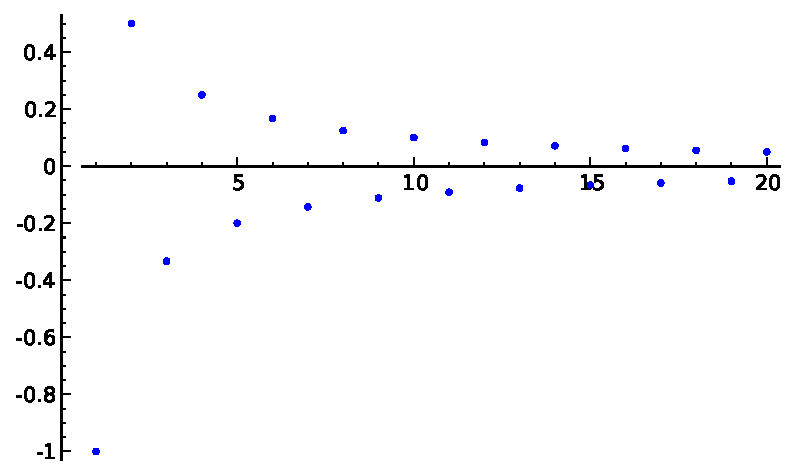
\includegraphics[width=9.5cm]{folge.pdf}
\end{center}
\subsubsection{Konvergenzkriterien}
Wir können folgende Aussagen bzgl der Konvergenz von Folgen machen:\\
Jede monotone, beschränkte Folge konvergiert.\\
Sind $(a_n)_n$ und $(b_n)_n$ konvergente Folgen, $\alpha, \beta \in \mathbb{R}$, so ist auch die
                   Folge $( \alpha a_n+\beta b_n)_n$ konvergent mit
                   dem Grenzwert
 \[ \lim_{n \rightarrow \infty} ( \alpha a_n + \beta b_n)= \alpha
                   \lim_{n \rightarrow \infty} a_n + \beta \lim_{n
                   \rightarrow \infty} b_n .\]
Sind $(a_n)_n$ und $(b_n)_n$ konvergente Folgen, so ist auch die
                   Folge $(a_n b_n)_n$ konvergent mit
                   dem Grenzwert
 \[
  \lim_{n \rightarrow \infty} ( a_n b_n)= 
                   (\lim_{n \rightarrow \infty} a_n) \cdot  (\lim_{n
                   \rightarrow \infty} b_n).
 \]
\begin{bem}
  Weglassen oder Hinzufügen endlich vieler Glieder verändert das
                   Konvergenzverhalten nicht.
\end{bem}
Wir möchten hier einge wichtige Sätze über Konvergenz anbringen:
\begin{sz}[Bolzano-Weierstrass]
Jede beschränkte Folge besitzt (mindestens) eine
konvergente Teilfolge.\\
 Jede Teilfolge einer konvergenten Folge konvergiert gegen den
Grenzwert der ursprünglichen Folge.\\
 Jede konvergente Folge ist beschränkt, d.h. es gibt ein $K>0$,
so dass $|a_n|\leq K$ gilt für alle $n \in \mathbb{N}$.\\
Seien $(a_n)_n$ und $(b_n)_n$ konvergente Folgen mit $\lim_{n
\rightarrow \infty} a_n = \lim_{n \rightarrow \infty} b_n$. Dann gilt
für eine Folge $(c_n)_n$ mit $a_n \leq c_n \leq b_n$, $n \in
\mathbb{N}$, dass sie konvergiert mit  $\lim_{n
\rightarrow \infty} c_n = \lim_{n \rightarrow \infty} b_n$. $(c_n)_n$ heißt Zwischenfolge.
\end{sz}
\subsubsection{Rekursive Folgen}
Rekursive Folgen können durch rekursive Funktionen erzeugt werden.
Wir betrachten exremplarisch die Folge 
\[ y_{n+2}:=2y_{n+1}-y_n+2, \quad y_0=-1, y_1=a. \]
\begin{sagein}
var('a')
def y(n):
   if n==0:
       return -1
   if n==1:
       return a
   return 2*y(n-1)-y(n-2)+2
y(4)
\end{sagein}
\begin{sage}
4*a + 15
\end{sage}
%%%%%%%%%%%%%%%%%%%%%%%%%%%%%%%%%%%%%%
\section{Reihen}
%%%%%%%%%%%%%%%%%%%%%%%%%%%%%%%%%%%%%%
Eng Verwandt mit Folgen sind Reihen, weshalb wir ebensolche nun hier betrachten wollen. Dazu einführend eine formale Definition.
\begin{df}
Sei $(a_n)_n$ eine Folge reeller Zahlen. Eine (unendliche)
Reihe mit den Gliedern $a_n$, in Zeichen
\[ \sum_{n=1}^\infty a_n =a_1 + a_2 + a_3 + \dots, \]
ist definiert durch die Folge $(s_n)_n$ der Partialsummen
\[
s_n=\sum_{k=1}^n a_k = a_1+a_2+ \dots +a_n 
\]
Der Grenzwert $s$ der Folge $(s_n)_n$ wird als Wert oder 
Summe der Reihe bezeichnet. Man schreibt
\[s= \sum_{n=1}^\infty a_n.\] 
\end{df}
\begin{bem}
Reihen sind eine spezielle Art von Folgen.\\
Indizierung mit $m$: $\sum_{n=m}^\infty a_n$.\\
Bei Abänderung, Weglassen oder Hinzufügen endlich vieler Glieder
bleiben Konvergenz und Divergenz unberührt. I.A. wird sich aber der
Grenzwert ändern.
\end{bem}
\subsubsection{Reihen in Sage}
Die Summe $\sum_{i=a}^b f(i)$ mit $a,b \in \mathbb{Z}$ lässt sich in Sage wie folgt erzeugen:
\begin{sagein}
sum(<f>,<i>,<a>,<b>) 
\end{sagein}
Gesucht ist hier eine geschlossene Darstellung der Summe $\sum_{i=a}^b f(i)$, dabei $a,b \in \mathbb{Z}$ ganze
Zahlen (auch unendlich (\isage{infinity/oo}), und \isage{f} ein Ausdruck in $i$.\\
Oft ist die Konvergenz einer Reihe abhängig von bestimmten Parametern. Je nach Parameterwert zeigt die Reihe
unterschiedliches Konvergenzverhalten.\\
%geometrische Reihe z.b.
Wir betrachten einige Beispiele.
Die geometrische Reihe ist gegeben durch $\sum_{n=0}^\infty x^n$. Die
Partialsummen lauten
\[ s_n=1+x+x^2+\ldots + x^n = \left \{ \begin{array}{ll}
n+1, & \mbox{ falls } x=1\\
\frac{1-x^{n+1}}{1-x}, & \mbox{ falls } x \neq 1 
\end{array} \right. .\]
Die Reihe divergiert für $|x|\geq1$ und konvergiert für $|x|<1$ mit
dem Wert $\sum_{n=0}^\infty = \frac{1}{1-x}$.
\begin{sagein}
sum(x^k,k,0,oo)
\end{sagein}
\begin{sage}
Is  abs(x)-1  positive, negative, or zero?
\end{sage}
Entsprechend gibt es keine geschlossene Form. Für $x=1/2$ gilt
\begin{sagein}
x = 1/2; sum(x^k,k,0,oo)
\end{sagein}
\begin{sage}
  2
\end{sage}
 Die Reihe $\sum_{n=1}^\infty \frac{1}{n^2}$ konvergiert gegen
$\pi^2/6$.
\begin{sagein}
_=var('k');sum(1/k^2,k,1,oo)
\end{sagein}
\begin{sage}
1/6*pi^2
\end{sage}
 Die alternierende harmonische Reihe  $\sum_{n=1}^\infty
\frac{(-1)^{n+1}}{n}$ konvergiert.
\begin{sagein}
sum((-1)^(k+1)/k,k,1,oo)
\end{sagein}
\begin{sage}
  log(2)
\end{sage}
 Die harmonische Reihe $\sum_{n=1}^\infty \frac{1}{n}$
 divergiert.
\begin{sagein}
sum(1/k,k,1,oo)
\end{sagein}
\begin{sage}
ValueError: Sum is divergent
\end{sage}
\subsubsection{Partialsummen}
Die Partialsumme einer Reihe lässt sich in Sage wie folgt definieren
\begin{sagein}
_=var('x,n,k')
s = sum(x^k,k,0,n); s
\end{sagein}
{\color{blue}\[\frac{x^{{\left(n + 1\right)}} - 1}{x - 1}\]}
% \begin{sage}
% (x^(n + 1) - 1)/(x - 1)
% \end{sage}
Die ersten $5$ Glieder der Partialsumme erhalten wir durch
\begin{sagein}
assume(x<>1); [s(n=m) for m in [1..6]]
\end{sagein}
{\color{blue}\[\left[\frac{x^{2} - 1}{x - 1}, \frac{x^{3} - 1}{x - 1}, \frac{x^{4} - 1}{x - 1}, \frac{x^{5} - 1}{x - 1}, \frac{x^{6} - 1}{x - 1}, \frac{x^{7} - 1}{x - 1}\right] \]}
% \begin{sage}
% [(x^2 - 1)/(x - 1), (x^3 - 1)/(x - 1), (x^4 - 1)/(x - 1), (x^5 - 1)/(x -
% 1), (x^6 - 1)/(x - 1), (x^7 - 1)/(x - 1)]
% \end{sage} 
Das Bestimmen des Grenzwertes der Folge der Partialsummen gelingt uns via
\begin{sagein}
forget();assume(abs(x)<1);limit(s,n=oo)
\end{sagein}
\begin{sage}
-1/(x - 1)
\end{sage}
\begin{sagein}
forget();assume(x>1);limit(s,n=oo)
\end{sagein}
\begin{sage}
+Infinity
\end{sage}
\subsubsection{\isage{assume()}}
Wir können Sage auffordern, bestimmte Annahmen über Variablen zu machen. Dafür haben wir den Befehl \isage{assume()}.
\begin{sagein}
assume(<assumptions>)
\end{sagein}
Wir betrachten ein Beispiel.
\begin{sagein}
assume(x,'real') # §$x$§ wird auf §$\mathbb{R}$§ eingeschränkt
assume(x>a) # §$x$§ wird auf  §$\{y \in \mathbb{R}\ |\ y>a\}$§ eingeschränkt
\end{sagein}
\begin{bem}
Ruft man \isage{assume()} mehrmals für einen Bezeichner auf, werden zusätzliche Annahmen gemacht. Sind diese
widersprüchlich erhält man eine entsprechende Meldung.
\end{bem}
Umformungen oder Vereinfachungen für symbolische Bezeichner
werden i.A. nur dann durchgeführt,
wenn sie für alle komplexen Zahlen gelten. Hier kann ein Einschränken
des Definitionsbereichs helfen.\\
 Mittels 
\begin{sagein}
forget(x>a)
\end{sagein}
wird die Annahme \isage{x>a} gelöscht.
 Durch 
\begin{sagein}
assumptions() 
\end{sagein}
können alle Annahmen ausgegeben werden.
% Durch den speziellen Bezeichner \isage{Global} können Annahmen
%für alle Bezeichner gesteuert werden. 
Wir betrachten weitere Beispiele.
\begin{sagein}
var('c'); assumptions()
\end{sagein}
\begin{sage}
c
[]
\end{sage}
\begin{sagein}
c = 2; assume(c>0)
\end{sagein}
\begin{sage}
 AttributeError: 'bool' object has no attribute 'assume'
\end{sage}
\begin{sagein}
_=var('c')
assume(c,'integer'); assumptions()
\end{sagein}
\begin{sage}
[c is integer]
\end{sage}
\begin{sagein}
sin(c*pi)
\end{sagein}
\begin{sage}
sin(pi*c)
\end{sage}
\begin{sagein}
sin(c*pi).simplify()
\end{sagein}
\begin{sage}
   0
\end{sage}
\begin{sagein}
assume(x>0)
sqrt(x^2).simplify()
\end{sagein}
\begin{sage}
  x
\end{sage}
% integer,
% noninteger, even, odd, rational, irrational, real, imaginary, complex,
% analytic, increasing, decreasing, oddfun, evenfun, posfun, constant,
% commutative, lassociative, rassociative, symmetric, antisymmetric,
% integervalued, one_to_one
Für \isage{assume()} stehen uns u.A. folgende Optionen zur verfügung:
\begin{center}
 \begin{tabular}{|l|l|}
\hline
Annahme & Erklärung\\
\hline
\isage{'real'} & $\mathbb{R}$ \\
\isage{'rational'} & $\mathbb{Q}$\\
\isage{'integer'} &  $\mathbb{Z}$\\
\isage{'complex'} & $\mathbb{C}$\\
\isage{'even'}   & gerade Zahl \\
\isage{'odd'} & ungerade Zahl\\
\isage{'increasing'} & wachsend \\
\isage{'analytic'} & analytisch\\
\hline
\end{tabular}
\end{center}
\subsubsection{Konvergenzkriterien II}
Wir reichen noch einige oft nützliche Konvergenzkriterien nach.\\
\begin{lm}[Cauchykriterium]
Eine Reihe $\sum_{n=1}^\infty a_n$ konvergiert
                  genau dann, wenn es zu jedem $\varepsilon>0$ ein $n_0
                  \in \mathbb{N}$ gibt, so dass für alle $m,n \geq n_0$
                  gilt $| \sum_{k=m}^n a_k|<\varepsilon$.
\end{lm}
\begin{lm}[Notwendiges Kriterium] Konvergiert eine Reihe, so bilden ihre Glieder eine Nullfolge. Dieses Kriterium ist nicht hinreichend!
\end{lm}
\begin{lm}[Verdichtungskriterium] Eine Reihe $\sum_{n=1}^\infty a_n$ mit
                  einer Folge nichtnegativer, monoton fallender
                  Glieder konvergiert genau dann, wenn die Reihe
                  $\sum_{n=1}^\infty 2^n a_{2^n}$ konvergiert.
\end{lm}
\begin{lm} Gilt $0 \leq c_n \leq a_n \leq b_n$ für alle $n \in \mathbb{N}$, so heißt 
\[\sum_{n=1}^\infty c_n \text{ Minorante für } \sum_{n=1}^\infty a_n\] 
\[\sum_{n=1}^\infty b_n \text{ Majorante für } \sum_{n=1}^\infty a_n\]
Die Reihe $\sum_{n=1}^\infty a_n$ konvergiert, wenn...
\begin{description}
\item[Majorantenkriterium] sie eine konvergente Majorante (mit nichtnegativen Gliedern) besitzt.
\item[Quotientenkriterium:] ihre Glieder positiv sind und ein $q<1$
existiert, so dass für $n \in \mathbb{N}$ gilt $\frac{a_{n+1}}{a_n}
\leq q$. 
\item[Wurzelkriterium:] ihre Glieder positiv sind und ein $q<1$
existiert, so dass für $n \in \mathbb{N}$ gilt $\sqrt[n]{a_n} \leq
q$. 
\item[Leibnizsches Kriterium:] sie bei $\sum_{n=1}^\infty (-1)^n a_n$
eine monoton fallende  Nullfolge ist.
\end{description}
Die Reihe $\sum_{n=1}^\infty a_n$ divergiert, wenn...
\begin{description}
\item[Majorantenkriterium:] sie eine divergente Minorante besitzt.
\end{description}
\end{lm}
Wir geben zwei Beispiele.\\
Betrachte $\sum_{n=0}^\infty n^4 e^{-n^2}$
\begin{sagein}
f(n) = n^4*exp(-n*n)
g(n) = f(n+1)/f(n)
limit(g(n),n=oo)
\end{sagein}
\begin{sage}
  0
\end{sage}
 Betrache $\sum_{n=2}^\infty \frac{1}{n (\log n)^2}$
\begin{sagein}
f(n) = 1/(n*(log(n)^2))
g(n) = 2^n*f(2^n)
h(n) = 2^n*g(2^n)
limit(h(n+1)/h(n),n=oo)
\end{sagein}
\begin{sage}
  1/2
 \end{sage}
\subsubsection{Absolute und bedingte Konvergenz}
Eine Reihe $\sum_{n=0}^\infty a_n$ heißt absolute konvergent
genau dann, wenn $\sum_{n=0}^\infty |a_n|$ konvergiert.\\
Eine konvergent, aber nicht absolut konvergente Reihe heißt bedingt konvergent.
\begin{bem}
 Absolut konvergente Reihen können beliebig umgeordnet werden.
 Dies ist i.d.R. für nicht absolut konvergenten Reihen falsch!
\end{bem}
%%%%%%%%%%%%%%%%%%%%%%%%%%%%%%%%%%%%%%
\section{Potenzreihen}
%%%%%%%%%%%%%%%%%%%%%%%%%%%%%%%%%%%%%%
Wir wollen uns spezielle Reihen, sog Potenzreihen anschauen. Diese sind gegeben durch
\[ \sum_{n=0}^\infty a_n (x-x_0)^n \]
mit $x_0 \in \mathbb{R}$. 
Eine Pontenzreihe besitzt einen sog Konvergenzradius, mit dem sich Aussagen über ihr Konvergenzverhalten machen lassen.
\begin{df}[Konvergenzradius]
\[  \rho := \frac{1}{ \limsup_{n \rightarrow \infty} \sqrt[n]{|a_n|}}
\]
Ist $a_n \neq 0$ für alle $n > n_0$:
\[
 \rho = \limsup_{n \rightarrow \infty} \frac{|a_{n}|}{|a_{n+1}|}.
\]
\end{df}
Für das Konvergenzverhalten gilt dann:\\
Die Potenzreihe konvergiert absolut für $|x -x_0|< \rho$.\\
Sie divergiert für $|x-x_0|>\rho$.\\
Über die Konvergenz an den Stellen $x_0-\rho$ und $x_0+\rho$ kann nichts gesagt werden. Diese müssen für 
jede Reihe individuell geprüft werden.   
Wir wollen uns dies an Beispielen verdeutlichen.\\
Sei $\sum_{n=1}^\infty \frac{x^n}{n!}$ gegeben und ihr Konvergenzradius von Interesse:
\begin{sagein}
f(n) = 1/factorial(n)
rho = limit(expand(f(n)/f(n+1)),n=oo); rho
\end{sagein}
\begin{sage}
+Infinity
\end{sage}
Die Potenzreihe konvergiert für alle $x \in \mathbb{R}$.\\ 
Sei nun $\sum_{n=0}^\infty n^s x^n$, $s>0$ gegeben und wieder der Konvergenzradius gefragt:
\begin{sagein}
_=var('s');f(n)= n^s; assume(s>0)
limit(expand(f(n)^(1/n)),n=infinity)
\end{sagein}
\begin{sage}
  1
\end{sage}
Der Konvergenzradius ist $1$.
\subsubsection{Exponentialfunktion}
Wir erklären die Exponentialfunktion durch
\[  exp(x) := \sum_{i=0}^\infty \frac{x^n}{n!}= 1 + \frac{x}{1!} +
\frac{x^2}{2!}+ \frac{x^3}{3!}+ \dots, x \in \mathbb{R}. \]
Die Funktion ist auf ganz $\mathbb{R}$ definiert. Der Graph der Funktion ist gegeben zu:
\begin{sagein}
plot(exp,(-5,5))
\end{sagein}
\begin{center}
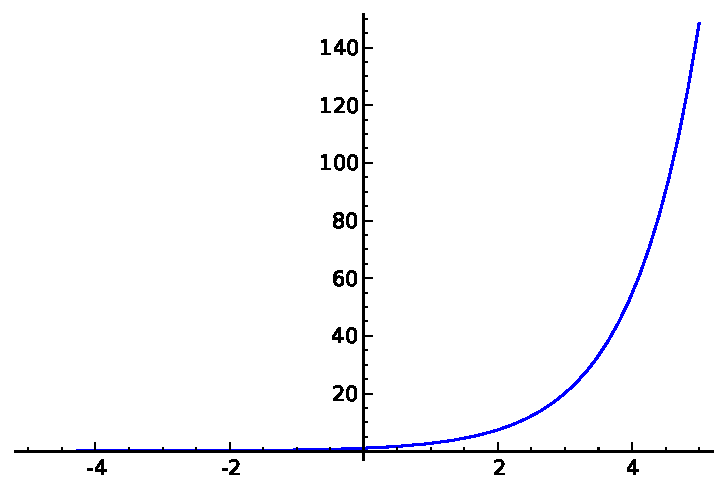
\includegraphics[width=6cm]{fexp.pdf}
\end{center}
Wir wollen uns an einige Eigenschaften der Exponentialfunktion erinnern:\\
Es gilt $\exp(x+y)=\exp(x) \cdot \exp(y)$.\\
Es gilt $\exp(x)=\lim_{n \rightarrow \infty} (1+\frac{x}{n})^n$.\\
Es gilt $\exp(x)=1/\exp(-x)$.\\
Die Umkehrfunktion auf $\mathbb{R}_+$ der Exponentialfunktion ist die
 Logarithmusfunktion $\log (x)$. Es gilt
\[ \exp(\log(x))=x, \ x >0, \quad \log ( \exp ( x ))=x, \ x \in \mathbb{R}.\] 
 Die allgemeine Potenz ist durch $a^x:=\exp( x \log a)$,
$a\in \mathbb{R}_+$
definiert. 
\subsubsection{Exponential- und Logarithmusfunktion in Sage}
Wie wir oben schon bemerkt haben könnten, ist die Exponentialfunktion in Sage gegeben durch
\begin{sagein}
sum(x^n/factorial(n),n,0,oo)
\end{sagein}
\begin{sage}
  e^x
\end{sage}
Wir testen, ob der Logarithmus die Umkehrung der Exponentialfunktion ist:
\begin{sagein}
exp(log(x))
\end{sagein}
\begin{sage}
  x
\end{sage}
Alternative darstellung der Exponentialfunktion:
\begin{sagein}
_=var('n');limit((1+x/n)^n,n=oo)
\end{sagein}
\begin{sage}
  e^x
\end{sage}
% \begin{sagein}
% ??
% ??
% \end{sagein}
% \begin{sage}
%   
% \end{sage}
\subsubsection{Trigonometrische Funktionen}
Die Sinusfunktion und die Cosinusfunktion sind definiert
durch
\begin{eqnarray*}
\sin(x) := \sum_{n=0}^\infty (-1)^n \frac{x^{2n+1}}{(2n+1)!} \quad\quad
\cos(x) := \sum_{n=0}^\infty (-1)^n \frac{x^{2n}}{(2n)!}. 
\end{eqnarray*}
Die Potenzreihen konvergieren für alle $x \in \mathbb{R}$. Wir machen uns ein Bild:
\begin{sagein}
p = plot(sin,0,4*pi,color='red')
p += plot(cos,0,4*pi); 
p += text('-- $\sin(x)$', (10, 1.0), color='red')
p += text('-- $\cos(x)$', (10, 0.85)); p.show()
\end{sagein}
\begin{center}
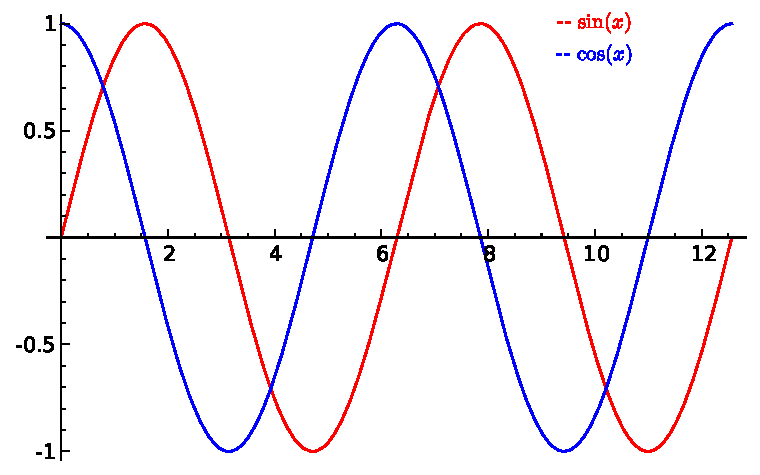
\includegraphics[width=5.5cm]{sincos.pdf}
\end{center}
Wir erinnern uns auch an einige Eigenschaften der trigonometrischen Funktionen. Da wären zuerst sicherlich die Additionstheoreme:
\begin{eqnarray*}
\sin(x+y) & = &\sin x \cos y+ \cos x \sin y \\
\cos(x+y) & = &\cos x \cos y - \sin x \sin y .
\end{eqnarray*} 
Es gelten folgende Identitäten: 
\[\sin^2x +\cos^2x=1.\]
 \begin{eqnarray*}
\sin(x+\pi/2)&=&\cos(x)\\
 \cos(x+\pi/2)&=&-\sin(x).
\end{eqnarray*} 
\begin{bem}
 Wir definieren $\pi$, indem wir die kleinste positive Nullstelle
von $\cos(x)$ als $\pi/2$ definieren.
\end{bem}
\subsubsection{Trigonometrische Funktionen in Sage}
Wir betrachten zwei kleine Beispiele:
\begin{sagein}
solve(cos(x)==0,x)
\end{sagein}
\begin{sage}
[x == 1/2*pi]
\end{sage}
\begin{sagein}
sin(x+pi/2).simplify()
\end{sagein}
\begin{sage}
cos(x)
\end{sage}
Wir wollen uns um weitere Eigenschaften der trigonometrischen Funktionen bemühen.
% Man kann die Sinusfunktion und die Cosinusfunktion mit Hilfe eines rechtwinkligen Dreiecks im Einheitskreis auch geometrisch  deuten.
Die Umkehrfunktion des Sinus ist $\arcsin$, die des Cosinus $\arccos$. Wiederum machen wir uns ein Bild: 
\begin{sagein}
p = plot(arcsin,-1,1,color='red')
p += plot(arccos,-1,1); 
p += text('-- arcsin(x)', (-0.7, 1.0), color='red')
p += text('-- arccos(x)', (-0.7, 0.75)); p.show()
\end{sagein}
\begin{center}
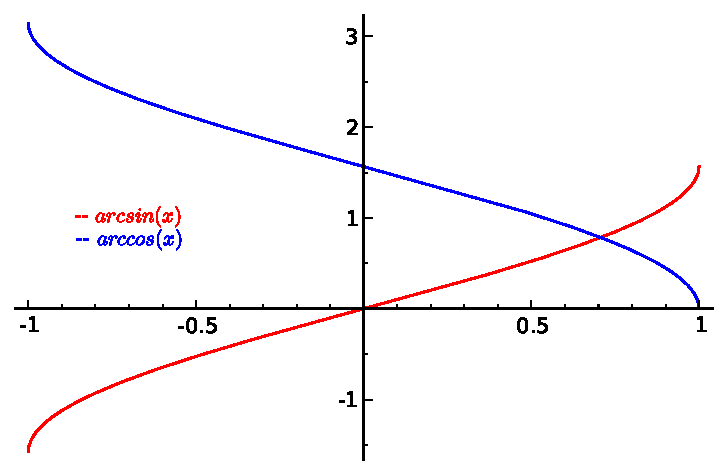
\includegraphics[width=6.5cm]{arcsinarccos.pdf}
\end{center}
Der Tangens ist definiert durch
$\tan(x) :=\frac{\sin(x)}{\cos(x)}$.
\begin{sagein}
plot(tan,-4,4,detect_poles=True,ymax=4,ymin=-4)
\end{sagein}
\begin{center}
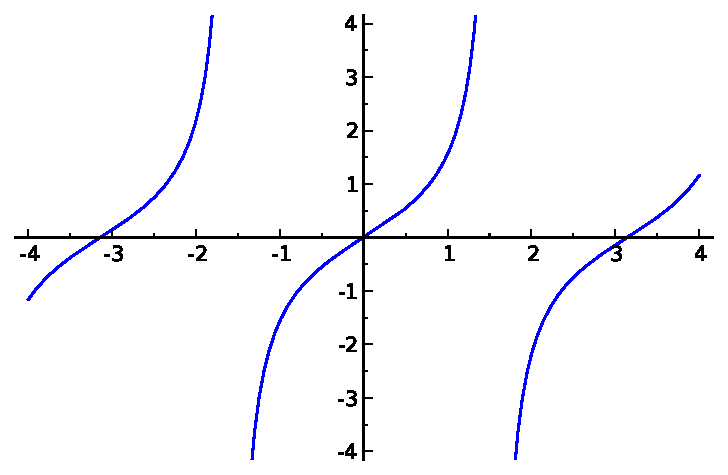
\includegraphics[width=7cm]{tan.pdf}
\end{center}
%%%%%%%%%%%%%%%%%%%%%%%%%%%%%%%%%%%%%%
\chapter{Vertiefung Schleifen}
%%%%%%%%%%%%%%%%%%%%%%%%%%%%%%%%%%%%%%
Wir wollen eine Alternative der uns bekannten \isage{for()}-Schleife betrachten, die \isage{while()}-Schleife:
\begin{sagein}
while <expression> :
    <Code-block>
\end{sagein}
Diese wiederholt \isage{<Code-block>} solange wie die \isage{<expression>} als 
\isage{True} ausgewertet wird.
Dazu betrachten wir ein Beispiel:
\begin{sagein}
f(x) = 1/x
x=0.1
while f(x) > 0.1:
    x += 0.1
x
\end{sagein}
\begin{sage}
 10.1000000000000
\end{sage}
%achtung: rundungsfehler, daher kommt 10.1 raus.. selbst einmal drauf reingefallen..
% 
%  Die Schleifenvariable $k$ durchläuft die Werte $1$, $2$, $3$ und
%   $4$. Dabei wird alles was ab \isage{:} eingerückt ist $k$-mal durchlaufen.
%  Ergebnisse, die in jedem Schleifenschritt berechnet werden,
%   werden \alert{nicht} auf dem Bildschirm ausgegeben. 
%  Eine Ausgabe wird durch den \isage{print}-Befehl erzielt.
% 
% \end{frame}

% \begin{frame}[fragile]{Schleifen III}
%  Eine elegante Möglichkeit sind Schleifen über Listen oder Mengen.
% \begin{sage}
% L = [1..10]
% for i in L:
%     x = i^2
%     print("Das Quadrat von {0} ist {1}").format(i,x)
% \end{sage}
% \end{frame}

% \begin{frame}[fragile]{Etwas Zahlentheorie}
% Wir geben für die natürlichen Zahlen $\leq 1000$ an, wieviele Zahlen
% $1,2,3,\dots $ Teiler haben.
% \begin{sagein}
% Liste = [1..1000]
% def anz_teiler(n): return len(divisors(n))
% Liste2 = map(anz_teiler,Liste)
% for k in [1..50]:
%     print "{0} , {1}".format(k,len(filter(lambda x: x == k, Liste2)))
% print divisors(840)
% \end{sagein}
Wir können Schleifen auch abwärts zählen (also ``umgekehrt'' durchlaufen):
\begin{sagein}
for j in reversed([2,4]):
   print("{0}, {1}").format(x,x^j) 
\end{sagein}
Nicht nur die Durchlaufrichtung ist variabel, sondern auch die Schrittweiten selbst können modifiziert werden:
\begin{sagein}
for j in srange(3,10,2.6):
    print(x,x^j) 
\end{sagein}
\begin{sage}
(x, x^3.00000000000000)
(x, x^5.60000000000000)
(x, x^8.20000000000000)
\end{sage}
\subsubsection{Fixpunkte}
Schon einmal wurde die Suche einer Nullstelle zurückgeführt auf die Bestimmung eines Fixpunktes- nur wie finden wir den Fixpunkt einer Funktion? Wir wollen die Idee 
eines Verfahrens zur Fixpunktbestimmung am Beispiel des $cos()$ erläutern. Wir suche ein $x_{\mathrm{fix}} \in \mathbb{R}$ so dass
\[ x_{\mathrm{fix}} = \cos (x_{\mathrm{fix}}) \]
gilt. Hierzu machen wir uns ein Bild:
\begin{center}
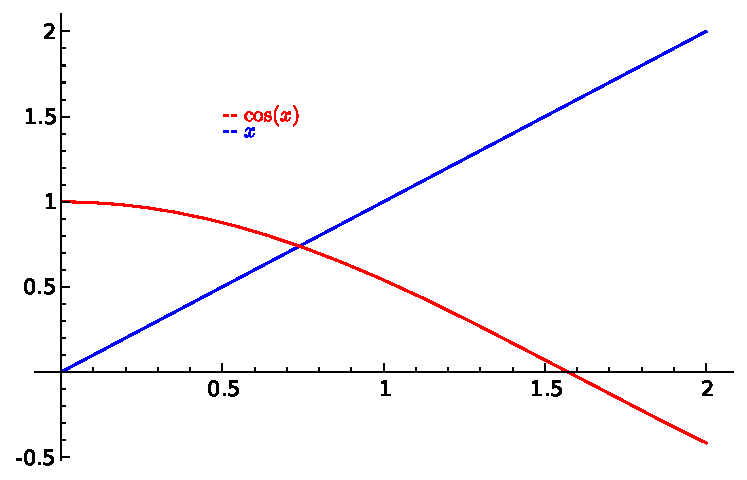
\includegraphics[width=8cm]{iter1.pdf}
\end{center}
\subsubsection{Fixpunkt-Iteration}
Die Fixpunkt-Iteration 
\[ x_{k+1}=cos(x_k) \]
bei geeignetem Startwert $x_0 = 0.2$ liefert den gesuchten Wert:
\begin{center}
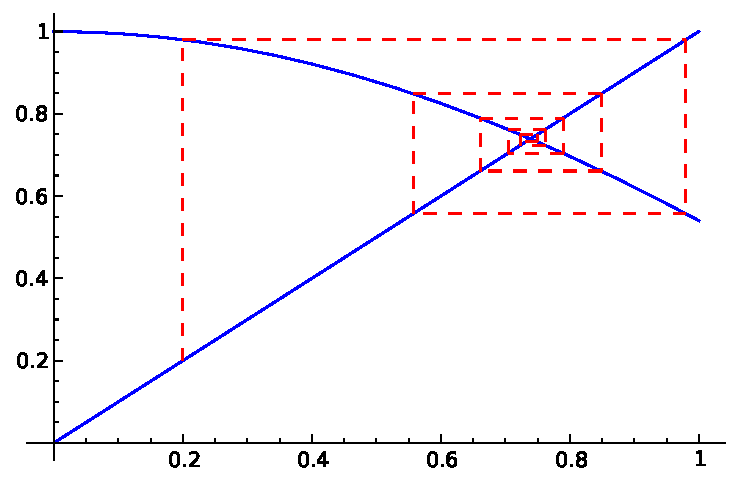
\includegraphics[width=8cm]{fixpunkt.pdf}
\end{center}
\subsubsection{Implementierung Fixpunkt-Iteration}
\begin{sagein}
def fixpunkt(f,In,x0,n):
    y = [x0]
    p = plot(f,(In[0],In[1]))
    p += plot(x,(In[0],In[1]))
    for i in [0..n-1]:
        y.append(float(f(y[i])))
        p += line( [ (y[i],y[i]), (y[i],y[i+1]) ],linestyle='--', color='red')
        p += line( [ (y[i],y[i+1]), (y[i+1],y[i+1]) ],linestyle='--', color='red')
    p.show()
    return(y)
\end{sagein}
Über folgenden Aufruf werden die Ergebnisse jedes Iterationsschritts zurückgeliefert- das letzte Ergebnis sollte also unsere Approximation des Fixpunkts sein.
\begin{sagein}
fixpunkt(lambda x: cos(x),[0,1],0.2,10)
\end{sagein}
\begin{sage}
[0.200000000000000, 0.98006657784124163, 0.55696725280964243, 0.84886216565827077, 0.66083755111661502, 0.78947843776686832, 0.70421571334199318, 0.76211956176066087, 0.72337417210557109, 0.74957657633149311, 0.73197742525819132]
\end{sage}
\begin{bem}
 Unsere Funktion approximiert den Fixpunkt beliebig schlecht (abhängig von der Größe unseres $n$, denn es werden eben ``nur'' $n$ Iterationen durchgeführt). Eine \isage{while()}-Schleife 
mit geeignetem Abbruchkriterium könnte Abhilfe schaffen. Der geneigten Leserin sei die Implementation als spaßige Übung nahegebracht.
\end{bem}
%%%%%%%%%%%%%%%%%%%%%%%%%%%%%%%%%%%%%%
\chapter{Funktionen(-folgen), Grenzwert und Stetigkeit}
\section{Funktionen}
%%%%%%%%%%%%%%%%%%%%%%%%%%%%%%%%%%%%%%
Wir wollen reelle Funktionen kennenlernen. Dazu eine Definition.
\begin{df}
Eine Abbildung
\[f: \ D \subset \mathbb{R} \ \rightarrow \ \mathbb{R}.\]
die jedem Element aus $D$ eindeutig genau ein Element aus $\mathbb{R}$ zuordnet heißt (reelle) Funktion.\\
$D \subset \mathbb{R}$, $D \neq \emptyset$ heißt Definitionsbereich von $f$.\\
Die Menge $f(D)$ aller rellen Zahlen, die als Werte der
Funktion vorkommen heißt Wertebereich von $f$.\\
Die Menge aller Punkte 
\[ \{ (x,f(x)) \in \mathbb{R}^2 \;|\; x \in D\}. \]
heißt Graph der Funktion $f$
\end{df}
Wie wir wissen, lassen sich zwei Funktionen $f$ und $g$ wie folgt verknüpfen:
\begin{sz}[Verknüpfung von Funktionen]
Seien $f$ und $g$ Funktionen mit einem gemeinsamen Definitionsbereich.\\
Die Summe von $f$ und $g$ ist definiert als $(f+g)(x):=f(x)+g(x)$.\\
Analoges gilt für die Differenz von $f$ und $g$: $(f-g)(x):=f(x)-g(x)$.\\
Das Produkt beider Funktionen ist gegeben zu $(f\cdot g)(x):=f(x) \cdot g(x)$.\\
Analog erhalten wir den Quotienten: $(\frac{f}{g})(x):=\frac{f(x)}{g(x)}$, falls $g(x) \neq
0$ für alle $x \in D$.\\
Durch $f:D_f \rightarrow \mathbb{R}$ und $g:D_g \rightarrow \mathbb{R}$, 
dabei $f(D_f) \subset D_g$ 
\[(g \circ f) (x):=g(f(x)).\] 
ist die Komposition von $f$ und $g$ definiert.
\end{sz}
Wie uns weiterhin bekannt ist, lassen sich FUnktionen auch mehrdimensional definieren.
\begin{df}[Mehrdimensionale Funktion]
Ist $D \subseteq \mathbb{R}^n$ und $f : D \Rightarrow \mathbb{R}$ dann spricht man von
einer reellen Funktion in mehreren Veränderlichen. Das Studium dieser Funktionen ist einer der Hauptinhalte der Diff2-Vorlesung.
\bigskip
Weiterhin können Funktionen auch Wertebereiche außerhalb der reellen Zahlen haben.
Z.B. 
\[f : D \Rightarrow \mathbb{R}^m.\]
Im physikalischen Umfeld spricht man für $m=1$ dann von skalarwertigen Funktionen und für $m>1$ von vektorwertigen Funktionen oder Vektorfeldern.
\end{df} 
\subsubsection{Funktionen in Sage}
Die Abbildung $f$ mit Argumenten $x,y$ lässt sich wie folgt erzeugen
\begin{sagein}
f(x,y,...) = expr
\end{sagein}
Wir betrachten eine konkrete Funktion $f$
\begin{sagein}
f(x,y) = x^2+y^2; f
\end{sagein}
\begin{sage}
(x, y) |--> x^2 + y^2
\end{sage}
Die so definierte Funktion $f$ kann wie jede beliebige andere Funktion
aufgerufen werden. Funktionen haben den Datentyp \isage{expression}.
\begin{sagein}
_=var('a,b');f(a,b+1)
\end{sagein}
\begin{sage}
(b + 1)^2 + a^2
\end{sage}
\begin{sagein}
type(f)
\end{sagein}
\begin{sage}
<type 'sage.symbolic.expression.Expression'>
\end{sage}
Wie gewohnt können Abbildungen addiert, subtrahiert, multipliziert und
dividiert werden:
\begin{sagein}
f(x) = 1/(1+x); g(x) = sin(x^2)
h = f+g; k = f*g; l = f/g
h(a),k(a),l(a)
\end{sagein}
{\color{blue} \[\left(\frac{1}{a + 1} + \sin\left(a^{2}\right),
\frac{\sin\left(a^{2}\right)}{a + 1}, \frac{1}{{\left(a + 1\right)}
\sin\left(a^{2}\right)}\right)\]}
% \begin{sage}
% (1/(a + 1) + sin(a^2), sin(a^2)/(a + 1), 1/((a + 1)*sin(a^2)))
% \end{sage}
\subsubsection{Komposition in Sage}
Kompositionen $f\circ g$ werden in Sage durch Ineinanderschachteln erzeugt:
\begin{sagein}
f_g(x) = f(g); g_f(x) = g(f)
f_g(x), g_f(x)
\end{sagein}
{\color{blue} \[ \left(\frac{1}{\sin\left(x^{2}\right) + 1}, \sin\left(\frac{1}{{\left(x
+ 1\right)}^{2}}\right)\right) \]}
% \begin{sage}
% (1/(sin(x^2) + 1), sin((x + 1)^(-2)))
% \end{sage}
Mehrfachverknüpfungen erhalten wir durch mehrfaches Hintereinanderschalten $f(f(\cdots f(\cdot)))=f \circ \dots
\circ f(\cdot)$
\begin{sagein}
g4(x) = g(g(g(g))); g4
\end{sagein}
{\color{blue} \[ x \ {\mapsto}\sin\left(\sin\left(\sin\left(\sin\left(x^{2}\right)^{2}\right)^{2}\right)^{2}\right) \]}
% \begin{sage}
% x |--> sin(sin(sin(sin(x^2)^2)^2)^2)
% \end{sage}
Diese Konstruktionen funktionieren auch mit Systemfunktionen:
\begin{sagein}
abs(real(-2+3*I))
\end{sagein}
\begin{sage}
  2
\end{sage}
Kompliziertere Funktionen können besser durch selbst definierte Funktionen/Prozeduren \isage{def <func>():} erklärt
werden (vgl. Kapitel 4).
\subsubsection{Ausdrücke und Funktionen}
Wir unterschedien zwischen der Funktion $f$ als Funktion $f(x)=expr(x)$ oder als Ausdruck $f=expr$. Der Typ ist identisch, 
die Funktionsauswertung i.A. allerdings unterschiedlich. Wir machen uns diesen Unterschied klar:
\begin{sagein}
Funktion(x) = 2*x*cos(x); Funktion(1)
\end{sagein}
\begin{sage}
  2*cos(1)
\end{sage}
\begin{sagein}
Ausdruck = 2*x*cos(x); Ausdruck(x=1)
\end{sagein}
\begin{sage}
  2*cos(1)
\end{sage}
Auch mehrere Veränderliche  sind möglich:
\begin{sagein}
_=var('y');Funktion2(x) = x+sin(y); Funktion2
\end{sagein}
\begin{sage}
 x |--> x + sin(y)
\end{sage}
\begin{sagein}
Funktion3(x,y) = x+sin(y); Funktion3
\end{sagein}
\begin{sage}
  (x, y) |--> x + sin(y)
\end{sage}
%%%%%%%%%%%%%%%%%%%%%%%%%%%%%%%%%%%%%%
\section{Grenzwerte und Stetigkeit}
%%%%%%%%%%%%%%%%%%%%%%%%%%%%%%%%%%%%%%
\subsection{Grenzwerte}
Wir wollen uns mit Grenzwerten von Funktionen befassen. Dazu folgende Definition.
\begin{df}[Grenzwert]
Sei $f$ eine Funktion mit Definitionsbereich $D$ und $a\in D$.\\
$f$ strebt für $x \rightarrow a$ gegen $b \in \mathbb{R}$, wenn es zu jedem $\varepsilon >0$ ein $\delta >0$ gibt, so
dass für alle $x \in D\smallsetminus\{a \}$ mit $|x-a|<\delta$ gilt 
\[ |f(x)-b| < \varepsilon .\]
Der Grenzwert $b$ ist eindeutig bestimmt und man schreibt
\[ \lim_{x \rightarrow a} f(x) =b \mbox{ oder } f(x) \rightarrow b
\mbox{ für } x \rightarrow a. \]
Die Aussage überträgt sich sinngemäß auf $a=\pm \infty$.
\end{df}
Wir fassen einige Tatsachen in einem Satz zusammen.
\begin{sz}
Nach dem Folgenkriterium gilt $ \lim_{x \rightarrow a} f(x) =b$
genau dann, wenn für jede Folge $a_n \in D$ mit $a_n \neq a$ und $a_n \rightarrow a$
gilt $\lim_{n \rightarrow \infty} f(a_n)=b$.\\
Es gelten die üblichen Rechenregeln:
\begin{eqnarray*}
\lim_{x \rightarrow a}(f(x)+g(x)) &=&\lim_{x \rightarrow a} f(x) +
\lim_{x \rightarrow a} g(x) \\
\lim_{x \rightarrow a}(f(x) \cdot g(x)) &=& \lim_{x \rightarrow a}
f(x) \cdot \lim_{x \rightarrow a} g(x)
\end{eqnarray*}
wenn $\lim_{x \rightarrow a} f(x)$ und $\lim_{x \rightarrow a}g(x)$
existieren.\\
Gilt $\lim_{x \rightarrow a} f(x)=b$, $\lim_{x \rightarrow b}
g(x)=c$ bei entsprechenden Definitionsgebieten für $f$ und $g$, so
folgt $\lim_{x \rightarrow a} g(f(x)) =c$.
\end{sz}
\subsubsection{limit()}
Sage stellt uns für Grenzwertbetrachtungen den uns bekannten \isage{limit()}-Befehl zur Verfügung:
\begin{sagein}
expr.limit(x = a, dir=None, taylor=False)
limit(expr, x = a, dir=None, taylor=False)
\end{sagein}
Hierdurch wird der (beidseitige) Grenzwert eines Ausdrucks mit der Unbekannten $x$ an
der Stelle $a$ bestimmt. $a$ kann auch $\pm \infty$ sein (\isage{infinity} oder \isage{oo}).\\
Wir haben die Möglichkeit, nur den linksseitigen bzw rechtsseitigen Grenzwert zu betrachten. Dazu müssen wir folgende Eisntellungen vornehmen:\\
\isage{dir='minus'} liefert uns den linksseitigen Limes.\\ 
Analog liefert \isage{dir='plus'} den rechtsseitigen Limes.\\
Sage kann die Grenzwertberechnung auch auf eine Taylorentwicklung stützen: \isage{taylor=True}. 
\subsubsection{Grenzwertrechnung in Sage}
Wir betrachten Grenzwerte einiger Beispiele.\\
$\lim_{x \rightarrow 0}
\frac{\sin(x)}{x}$
\begin{sagein}
limit(sin(x)/x,x=0)
\end{sagein}
\begin{sage}
  1
\end{sage}
$\lim_{x \rightarrow \infty}
\frac{\log(x)}{x}$
\begin{sagein}
limit(log(x)/x,x=infinity)
\end{sagein}
\begin{sage}
  0
\end{sage}
$\lim_{x \rightarrow \infty} \sqrt[x]{x}$
\begin{sagein}
limit(x^(1/x),x=infinity)
\end{sagein}
\begin{sage}
  1
\end{sage}
$\lim_{x \rightarrow 0}
\sin(1/x)$
\begin{sagein}
limit(sin(1/x),x=0)
\end{sagein}
\begin{sage}
  ind
\end{sage}
Der Grenzwert existiert nicht: \isage{ind} (indefinit aber beschränkt).\\ 
$\lim_{x \rightarrow 0} |x|' $
\begin{sagein}
limit(diff(abs(x),x),x=0),
limit(diff(abs(x),x),x=0,dir='minus'),
limit(diff(abs(x),x),x=0,dir='plus')
\end{sagein}
\begin{sage}
  (und, -1, 1)
\end{sage}
\subsection{Stetigkeit}
Wir definieren die Stetigkeit einer Funktion wie folgt.
\begin{df}[Stetigkeit]
Eine Funktion $f:D \ \rightarrow  \ \mathbb{R}$ heißt stetig an
der Stelle $x_0 \in D$, wenn es zu jedem $\varepsilon>0$ ein $\delta>0$
gibt, so dass für alle $x \in D$ mit $|x - x_0| < \delta$ gilt
\[ |f(x)-f(x_0) | < \varepsilon .\]
Man sagt, dass $f$ stetig ist, wenn $f$ an jeder Stelle $x_0
\in D$ stetig ist. \\
Sind $f$ und $g$ an $x_0$ stetig, so auch $f+g$, $f-g$, $f \cdot g$
und $\frac{f}{g}$ (falls $g(x_0) \neq 0$). 
\end{df}
Wir formulieren einige wichtige Sätze über Stetigkeit von Funktionen.
\begin{sz}
 Sei $f$ auf einem offenen Intervall $I$ definiert. $f$ ist an
$x_0 \in I$ genau dann stetig, wenn gilt
\[ \lim_{x \rightarrow x_0} f(x) = f(x_0). \]
 Für $f:I \rightarrow \mathbb{R}$ und $g:J \rightarrow
\mathbb{R}$ gelte $f(I) \subset J$ und es seien $f$ an $x_0 \in I$ und
$g$ an $y_0=f(x_0)$ stetig. Dann ist $g \circ f$ an $x_0$ stetig.\\
Eine Funktion $f: D \rightarrow \mathbb{R}$ ist linksstetig bzw. rechtsstetig, wenn $f|_{D\cap (-\infty,x_0)}$
bzw  $f|_{D\cap (x_0,\infty)}$ an $x_0$ stetig ist.\\
Eine Funktion $f$ ist dann an $x_0$ stetig, genau dann wenn $f$ links- und rechtsstetig
an $x_0$ ist.\\
Eine stetige Funktion auf einem abgeschlossenen Intervall $I=[a,b]$
besitzt ein Maximum und ein Minimum.\\
Eine stetige Funktion $f$ auf einem abgeschlossenen  Intervall
$[a,b]$ nimmt in $I$ jeden Wert zwischen $f(a)$ und $f(b)$ an.\\
Potenzreihen $f(x)=\sum_{n=0}^\infty a_n (x-x_0)^n$ sind stetig
innerhalb ihres Konvergenzintervalls.
\end{sz}
\subsubsection{Gleichmäßige Stetigkeit}
Wir wollen den Begriff der gleichmäßigen Stetigkeit definieren:
\begin{df}[Gleichmäßige Stetigkeit]
$f: D \rightarrow \mathbb{R}$ heißt gleichmäßig stetig auf $D$,
wenn es zu jedem $\varepsilon >0$ ein $\delta>0$ gibt, so dass für alle
Paare $x,x_0 \in D$ mit $|x - x_0|< \delta$ gilt
\[ | f(x)-f(x_0)| < \varepsilon. \]
\end{df}
\begin{bem}
 Die Exponentialfunktion ist auf jedem kompakten Intervall
gleichmäßig stetig (aber nicht auf ganz $\mathbb{R}$).\\
 $\log:(0,1) \rightarrow \mathbb{R}$ ist stetig aber nicht
gleichmäßig stetig.
\end{bem}
\subsubsection{Stetigkeit in Sage}
Um Stetigkeit einer Funktion $f$ an einer Stelle $x_0$feststellen zu können, bestimmen wir den linksseitigen und rechtsseitigen Grenzwerte:
\begin{sagein}
limit(1/x,x=0,dir='plus') 
\end{sagein}
\begin{sage}
 +Infinity
\end{sage}
\begin{sagein}
 limit(1/x,x=0,dir='minus')
\end{sagein}
\begin{sage}
 -Infinity
\end{sage}
%%%%%%%%%%%%%%%%%%%%%%%%%%%%%%%%%%%%%%
\section{Funktionenfolgen}
%%%%%%%%%%%%%%%%%%%%%%%%%%%%%%%%%%%%%%
Wir wollen Funktionenfolgen betrachten. Dazu definieren wir formal:
\begin{df}
Seien $f_n: D \ \rightarrow \ \mathbb{R}$, $n \in
\mathbb{N}$  rellwertige Funktionen auf  $D \subset \mathbb{R}$.\\
Dann heißt  $(f_n)_n$ Funktionenfolge.\\
Ist für jedes $x\in D$ die Folge $(f_n(x))_n$ konvergent, so wird durch 
\[ f(x):= \lim_{n \rightarrow \infty} f_n(x), \quad x \in D \]
die Grenzfunktion $f:D \ \rightarrow \ \mathbb{R}$ definiert.\\
Man sagt $f_n$ strebe punktweise auf $D$ gegen $f$.\\  
Durch $\sum_{i=1}^\infty f_i$ definierte Funktionenreihen
sind spezielle Funktionenfolgen.
\end{df}  
\subsubsection{Grenzübergänge}
Wir betrachten Grenzübergänge von Funktionenfolgen an einigen Beispielen:
$x^n \rightarrow 0$ auf dem Intervall $(-1,1)$.\\
$\left( 1+ \frac{x}{n} \right)^n \rightarrow \exp(x)$ auf $\mathbb{R}$.\\
Potenzreihen konvergieren innerhalb ihres Konvergenzradius.\\
Grenzprozesse lassen sich iA nicht vertauschen. Wir betrachten für $x \in (0,1)$:
\[ \lim_{x \rightarrow 1} \lim_{n \rightarrow \infty} x^n =0 \neq 1 = 
  \lim_{n \rightarrow \infty} \lim_{x \rightarrow 1} x^n.\]  
\subsubsection{Gleichmäßige Konvergenz}
Wir definieren gleichmäßige Konvergenz für Funktionenfolgen:
\begin{df}[Gleichmäßige Konvergenz]
$(f_n)_n$ konvergiert gleichmäßig auf $D$ gegen $f$, wenn es zu
jedem $\varepsilon >0$ ein $n_0 \in \mathbb{N}$ gibt, so dass für alle
$x \in D$ und $n\geq n_0$ gilt:
\[ |f_n(x) -f(x)| < \varepsilon.\]
\end{df}
Wir formulieren eine interessante Tatsache in einem Satz:
\begin{sz}
 Konvergiert $(f_n)_n$ gleichmäßig auf $D$ und existiert $\lim_{x
\rightarrow a} f_n(x)$ für $a\in D$, so gilt:
\[ \lim_{x \rightarrow a} \lim_{n \rightarrow \infty} f_n(x) = \lim_{n
\rightarrow \infty} \lim_{x \rightarrow a} f_n(x). \]
\end{sz}
\begin{bem}
 Die Grenzfunktion einer gleichmäßig konvergenten Folge stetiger
Funktionen ist stetig.\\
Ist $f_1, f_2, \ldots$, eine Folge von Funktionen auf $D \subseteq \mathbb{R}$, dann definiert
\[
 s := \sum_{n=1}^\infty f_n
\]
eine Funktionenreihe. Alle Aussagen übertragen sich analog; ebenso die Aussagen über die Folge der Partialsummen
\[
 s_k := \sum_{n=1}^k f_n.
\]
\end{bem}
 %%%%%%%%%%%%%%%%%%%%%%%%%%%%%%%%%%%%%%
\chapter{Grafik}
%%%%%%%%%%%%%%%%%%%%%%%%%%%%%%%%%%%%%%
Wir wollen uns etwas ausführlicher als bisher mit Grafiken befassen. Dazu stellen wir Folgendes fest:\\
Grafiken werden im Notebook integriert.\\
3D-Grafiken können interaktiv bearbeitet werden.\\
Grafikbefehle erzeugen grafische Objekte wie Geraden, Funktionsgraphen oder Kurven.\\
Zur Darstellung einer Grafik liefert Sage uns folgenden Befehl: \isage{<grafikobjekt>.show()} (oder letzte Zeile).\\
Beim Speichern unterscheiden wir 2D und 3D Grafiken:
\begin{itemize}
\item[2D] \isage{<grafikobjekt>.save('filename.extension')} speichert im Format \isage{<extension>}
\item[3D] \glqq{}Get Image\grqq{}-Link unter der Grafiken liefert Bitmap.
\end{itemize}
Es existieren eine Reihe spezialisierter Plot-Funktionen (Pfeile, Kugel, etc.)
\subsubsection{Optionen für grafische Objekte}
\begin{tabular}{lp{8cm}}
\isage{linestyle}  & Darstellung von Linien
           (\isage{'-'} (solid), \isage{'-.'} (dashed), \isage{':'}) (dotted)
                {\color{blue} \isage{linestyle = '.'}}\\
\isage{thickness}  & Linienstärke in mm
              {\color{blue} \isage{thickness = 4}}\\
\isage{color}      & Zuweisung einer Farbe
              {\color{blue} \isage{color='red'}}\\
\isage{plot_points}        & Anzahl Stützstellen
              {\color{blue} \isage{plot_points  = [nx,ny]}} (2 Parameter)\\
\isage{alpha/opacity}  & Transparenzfaktor
     {\color{blue} \isage{alpha = 0.8}}\\
\end{tabular}
\subsubsection{Ausgewählte Optionen für grafische Szenen}

\begin{tabular}{lp{8cm}}
\isage{aspect_ratio} & Verhältnis der Achsen (Breite/Höhe). $1$ für 1:1 Verhältnis. 
              {\color{blue} \isage{aspect_ratio = 2}}\\
\isage{figsize}    & Grösse des Bildes 
                  {\color{blue} \isage{figsize = [width, height]}}\\          
\isage{axes_labels} &  Tuple oder Liste der Achsenbeschriftungen 
{\color{blue} \isage{axes_labels = ('$x$','$y$')}}\\
\isage{gridlines} & Gitterlinien
              {\color{blue} \isage{gridlines = True}}
\end{tabular}
\subsubsection{plot()}
Da wir nun einige neue Erkenntnisse gewonnen haben, wollen wir das Plotten skalarer Funktionen  
$f:\mathbb{R}^n \ \rightarrow \mathbb{R},\, n=2,3$ betrachten. Das Schema eines Plots der Funktion $f$ im Intervall $x \in [a,b]$ bzw. $(x,y) \in [a,b] \times [c,d]$ hat folgende Gestalt:
\begin{sagein}
plot(f2,(x,a,b),optionen,...)
plot3d(f3,(x,a,b),(y,c,d),optionen,...)
\end{sagein}
\begin{bem}
 Die Angabe des Intervalls ist optional. 
 \isage{plot.options} gibt die Default-Optionen aus (2D).
\end{bem}
Wir betrachten einige Beispiele, sowohl 2D als auch 3D.
\subsubsection{2D-Plots}
\begin{sagein}
plot(x^2-1)
plot(sin(1/x),(x,-1,1))
plot(sin(1/x),(x,-1,1),adaptive_recursion=0)
\end{sagein}
\begin{bem}
 Diese Eingabe hätte die grafische Ausgabe des Graphen der Funktionen $sin(1/x)$ im Intervall $[-1,1]$ zur Folge.
\end{bem}
Es ist auch möglich, mehrere Funktionen im selben Plot darzustellen:
\begin{sagein}
p = plot(sin(x),color='red',xmin=-pi,xmax=pi)
p += plot(cos(x),xmin=-pi,xmax=pi); p.show()
\end{sagein}
\begin{center}
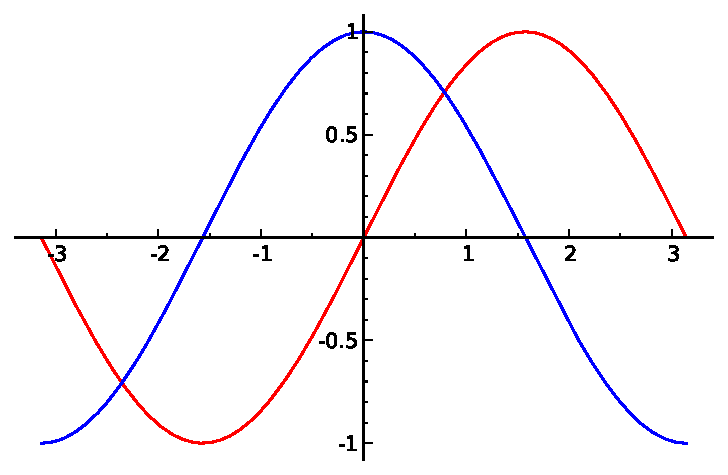
\includegraphics[width=6cm]{sincos2.pdf} 
\end{center}
\subsubsection{3D-Plots}
Wir wenden uns nun den 3D-Plots zu und benutzen als Beispiel die Funktion 
$f(x,y)=\sin(y^2+x)-\cos(y-x^2)$ auf $[0,\pi]^2$:
\begin{sagein}
f(x,y) = sin(y^2+x)-cos(y-x^2)
plot3d(f,(x,0,pi),(y,0,pi))
plot3d(f,(x,0,pi),(y,0,pi),plot_points=[10,10])
\end{sagein}
\begin{bem}
 Die resultierende Ausgabe wurde an dieser Stelle weggelassen.
\end{bem}
\medskip
Als weiteres Beispiel betrachten wir den Plot von $f(x,y)=\cos (20 \exp(-x^2-y^2 ))$ auf $[-1,1] \times [-1,1]$:
\begin{sagein}
g(x,y) = cos(20*exp(-x^2-y^2))
plot3d(g,(x,-1,1),(y,-1,1))
plot3d(g,(x,-1,1),(y,-1,1),plot_points=[80,80])
\end{sagein}
\begin{center}
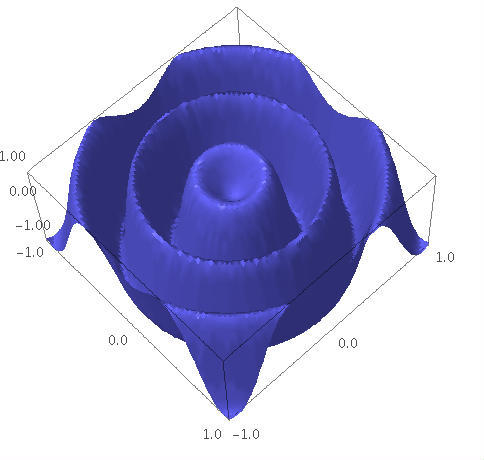
\includegraphics[width=4cm]{cosexp_trim.jpg} 
\end{center}
Als letztes Beispiel der 3D-Serie betrachten wir:
\begin{sagein}
W = plot3d(sin(pi*((x)^2+(y)^2))/2,(x,-1,1),(y,-1,1), frame=False, color='purple', opacity=0.8) 
S = sphere((0,0,0),size=0.3, color='red', aspect_ratio=[1,1,1])
show(W + S, figsize=8)
\end{sagein}
\begin{center}
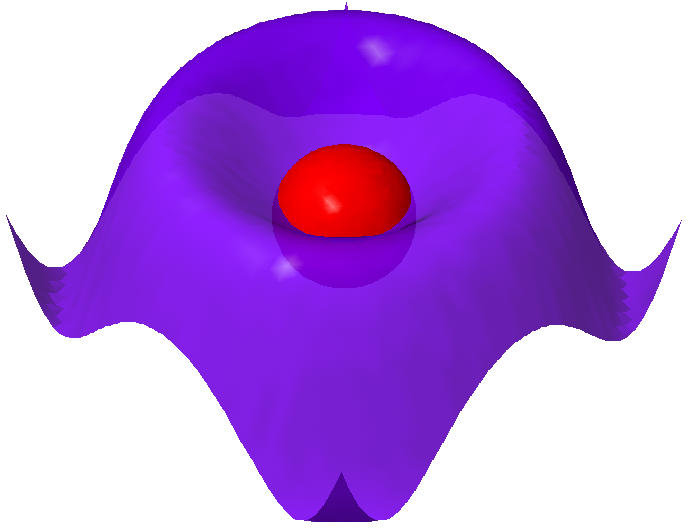
\includegraphics[width=7cm]{ball.jpg} 
\end{center}
\subsubsection{Kurven}
Wir beschäftigen uns nun mit Kurven und erinnern zunächst an die Parameterdarstellung: 
\[
 \{(x(t),y(t)) \in \mathbb{R}^2 \;|\; t \in [a,b]\}.
\]
\[
 \{(x(t),y(t),z(t)) \in \mathbb{R}^3 \;|\; t \in [a,b] \}.
\]
%Graph einer Funktion $f(x)$, $x \in [a,b]$: $t,f(t)$ mit  $t \in [a,b]$. 
Sage stellt uns hierfür folgendes Schema bereit:
\begin{sagein}
parametric_plot([x(t),y(t)], (t,a,b), optionen, ...)
parametric_plot([x(t),y(t),z(t)], (t,a,b), optionen, ...)
\end{sagein}
%$x$, $y$ und $z$ sind Ausdrücke mit der Unbekannten $t$. 
\subsubsection{2D-Kurven}
Wir betrachten Bespiele zweidimensionaler Kurven:
\begin{sagein}
_=var('t');f1 = parametric_plot([t,sin(t)],(t,0,2*pi),color='red')
f2 = parametric_plot([t,cos(t)],(t,0,2*pi),color='green')
f3 = parametric_plot([cos(t),sin(t)],(t,0,2*pi))
(f1+f2+f3).show(figsize=7)
\end{sagein}
\begin{center}
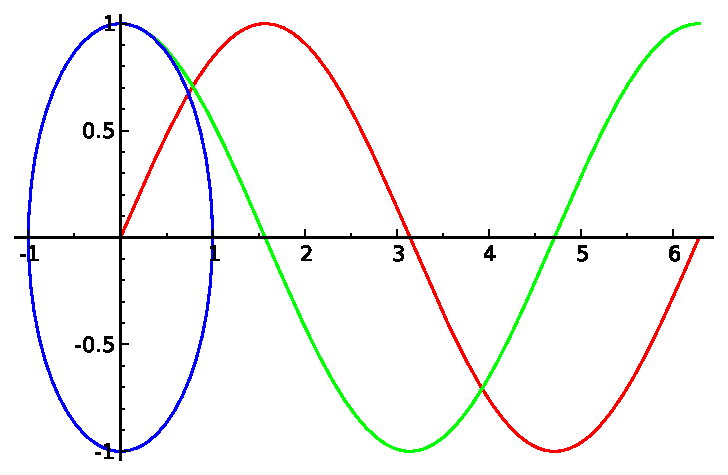
\includegraphics[width=7cm]{parametric2d.pdf} 
\end{center}
Wir wollen einen Kreis durch Punkte approximieren:
\begin{sagein}
[parametric_plot([cos(t),sin(t)],(t,0,2*pi),plot_points=2*k+1,randomize=False,adaptive_recursion=0 ) for k in [2..10]]
\end{sagein}
\begin{center}
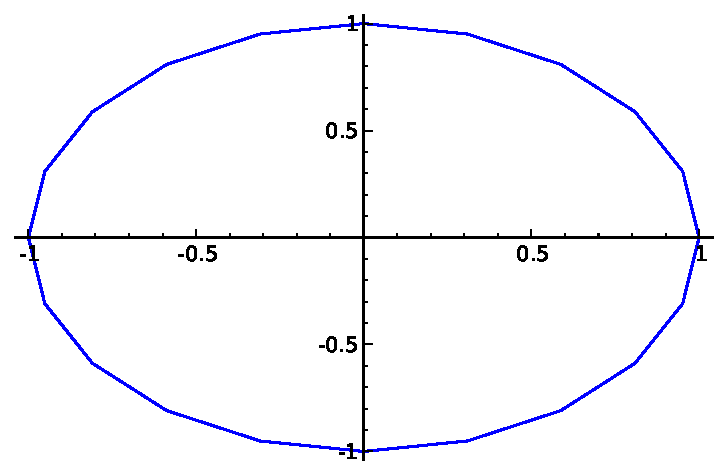
\includegraphics[width=7cm]{parametric2d_2.pdf} 
\end{center}
\begin{bem}
 Es werden 8 Kreise ausgegeben- für eine größe Genauigkeit muss die Range für $k$ größer gewählt werden.
\end{bem}
\subsubsection{3D-Kurven}
Wie uns wenig überrascht, beherrscht Sage auch Kurven, die dreidimensionale Gestalt haben. Wir betrachten folgendes kleine Beispiel:
\begin{sagein}
parametric_plot([(1-t*t)*cos(99*t),(1-t*t)*sin(99*t),t], (t,0,1),plot_points=400)
\end{sagein}
\begin{center}
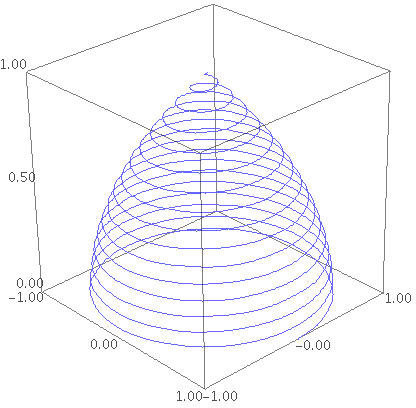
\includegraphics[width=7cm]{parametric3d.jpg} 
\end{center}
\subsubsection{Flächen}
Auch im Zusammenhang mit Fläche des $\mathbb{R}^3$ erinnern wir uns an die Parameterdarstellung:
\[
 \{(x(t1,t2),y(t1,t2),z(t1,t2)) \in \mathbb{R}^3 \;|\; t1 \in [a,b], t2 \in [c,d] \}.
\]
Das Sage-Schema sieht dann wie folgt aus:
\begin{sagein}
parametric_plot([x(t1,t2), y(t1,t2), z(t1,t2)], (t1,a,b), (t2,c,d), optionen, ...)
\end{sagein}
%  Beispielsweise lassen sich Graphen von Funktionen $f:[a
%    ,b]\times [c,d]
%    \ \rightarrow \ \mathbb{R}$ als Flächen
% \[ x=t_1, \ y=t_2, \ z=f(t_1,t_2) \]
% mit $a \leq t_1 \leq b, \ c \leq
%    t_2 \leq d$ erklären.
Wir betrachten bespielhaft eine Ellipsoid-Oberfläche
\[ 
x=r \cos(t_1) \sin(t_2), \ y=2r \sin (t_1) \sin (t_2),\ z =r \cos(t_2) 
\]
 mit $0 \leq t_1 \leq 2 \pi, 0 \leq t_2 \leq \pi.$ 
\begin{sagein}
_=var('t1,t2');r=1
x=r*cos(t1)*sin(t2)
y=2*r*sin(t1)*sin(t2)
z=r*cos(t2)
parametric_plot3d([x,y,z],(t1,0,2*pi),(t2,0,pi),aspect_ratio=1)
\end{sagein}
\begin{center}
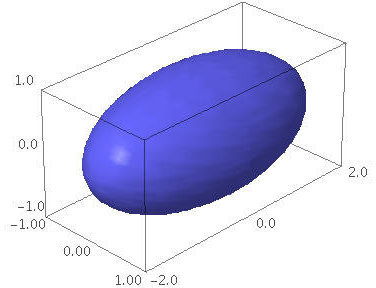
\includegraphics[width=4.5cm]{surface.jpg} 
\end{center}
\subsubsection{Kontur}
Wir betrachten noch zweidimensionale Grafiken für $f:\mathbb{R}^2 \rightarrow \mathbb{R}$:
\emph{Niveaulinien} (z.B. Höhenmeter auf einer
Landkarte):
\[ 
\{(x,y) \in \mathbb{R}^2 \;|\; f(x,y)=c, c \in \mathbb{R}\}
\]
Sage stellt uns hierfür den \isage{contour_plot}:
\begin{sagein}
contour_plot(f, (x,a,b), (y,c,d), contours=[c1,c2,...], optionen, ...)
\end{sagein}
Dabei geben $c1,c2,\ldots$ die entsprechenden Niveaulinien an.
Wir haben noch folgende Optionen:
\begin{itemize}
 \item \isage{fill=True}: Fläche zwischen den Linien ausfüllen.
 \item \isage{labels=True}: Automatische Kennzeichnung der Konturlinien.
\end{itemize}
Wir betrachten als Beispiel das Zeichnen der Niveaulinien für $-0.5, 0, 0.5$ der Funktion $\sin(4\pi x)y$: 
\begin{sagein}
contour_plot(sin(pi*4*x)*y,(x,-1,1),(y,-1,1),contours = [-0.5, 0, 0.5],fill=False,labels=True)
\end{sagein}
\begin{center}
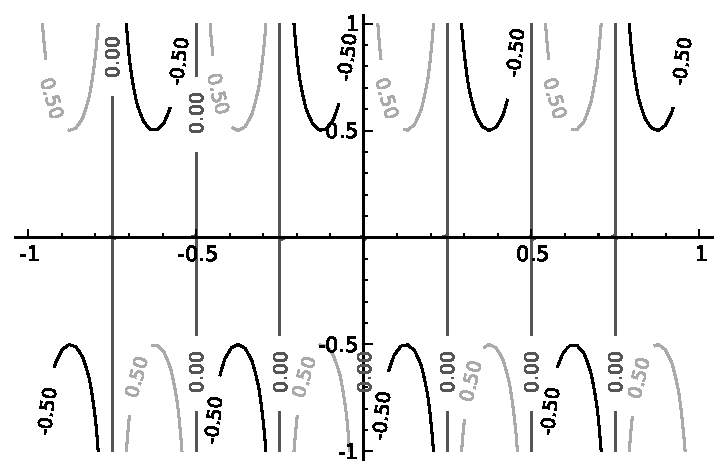
\includegraphics[width=7.5cm]{contour.pdf} 
\end{center}
\subsubsection{point()}
Ein oft nützliches Tool ist das Zeichnen von Punkten. Hierfür stellt Sage den Befehl {\color{blue} \isage{point()}}. 
Wir betrachten folgendes kleine Beispiel:
\begin{sagein}
point([(i,sin(i*6.28/50)) for i in [0..50]],color='red', pointsize=30) 
point2d.options
\end{sagein}
\begin{center}
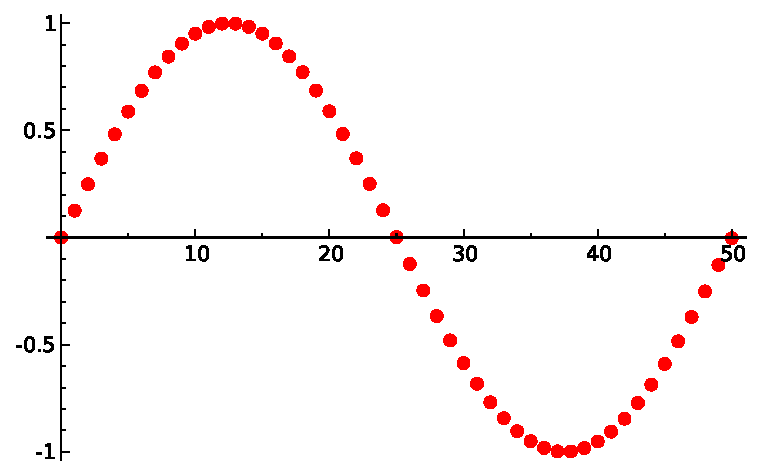
\includegraphics[width=7cm]{point2d.pdf} 
\end{center}
\subsubsection{Collatz Problem}
Wir wenden {\color{blue} \isage{point()}} auf ein komplizierteres Problem an:
Sei $x_0\in \mathbb{N}$. Dann definiert man die folgende Folge
\[ x_n:= \left \{ \begin{array}{ll}
 x_{n-1}/2, & \mbox{falls } x_{n-1} \mbox{ gerade ist} \\
3x_{n-1}+1 & \mbox{falls } x_{n-1} \mbox{ ungerade ist} 
\end{array} \right. . \] 
Man kann zeigen, dass für alle Startwerte ein $N_0$ existiert mit $x_{N_0}=1$.
\begin{sagein}
def collatz(n):
    """ Collatz problem """
    sequence = [n]; next_value = n;
    while next_value > 1:
        if next_value % 2 == 0:
            next_value = next_value/2
        else:
            next_value = 3*next_value+1
        sequence.append(next_value)
    Objekt = point([(i,sequence[i]) for i in [0..len(sequence)-1] ]) 
    Objekt.show()   
    return sequence
\end{sagein}
\begin{center}
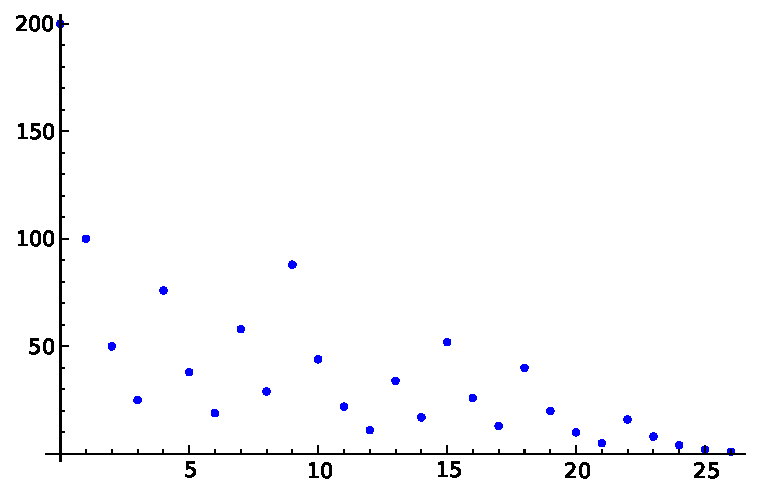
\includegraphics[width=5cm]{collatz.pdf} 
\end{center}
\subsubsection{animate()}
Der Befehl 
\begin{sagein}
animate([<graph1,graph2,...>], optionen, ... ) 
\end{sagein}
erstellt Animationen aus 2D plots. Wir haben die folgenden Optionen: \isage{xmin, xmax, ymin, ymax}.
Wir betrachten ein Beispiel:
\begin{sagein}
a = animate([plot(a*x^2, (x,-5,5)) for a in [-10..10]],ymin=-100,ymax=100)
a.show(iterations=1)
\end{sagein}
\begin{center}
 %\animategraphics[height=4cm]{2}{anime_}{0}{20}
\end{center}
%  Dreidimensionales Beispiel
% \begin{sagein}
% plotfunc3d(cos(j^0.5*PI*exp(-x^2-y^2)), 
%    x=-1..1, y=-1..1, j=1..30, Mesh=[40,40])
% \end{sagein}
%%%%%%%%%%%%%%%%%%%%%%%%%%%%%%%%%%%%%%
\chapter{Differentiation, Taylorsche Formel, Integration}
\section{Differentiation}
%%%%%%%%%%%%%%%%%%%%%%%%%%%%%%%%%%%%%%
Wir beginnen den Abschnitt mit einer formalen Definition:
\begin{df}
Eine Funktion $f: D \ \rightarrow \mathbb{R}$ heißt differenzierbar an
der Stelle $x_0 \in D$, wenn 
\[ \lim_{x \rightarrow x_0} \frac{f(x)-f(x_0)}{x -x_0} \]
existiert. \\
Der Grenzwert wird Ableitung oder Differentialquotient
von $f$ an $x_0$ genannt und mit $f\,'(x_0)=f^{\,(1)} (x_0)$ bezeichnet.
\end{df}
Wir machen einige Bemerkungen.
\begin{bem}
 $f$ ist differenzierbar (auf $D$), wenn $f$ an jeder
Stelle von $D$ differenzierbar ist. 
% {\color{red} Ableitung} von $f$: $f\,'$ für die gilt $f$ differenzierbar auf $D$.
 Eine Funktion $f:D \rightarrow \mathbb{R}$ ist an $x_0 \in D$
genau dann differenzierbar, wenn es eine lineare Abbildung
$T:\mathbb{R} \rightarrow \mathbb{R}$ gibt, so dass 
\[ f(x_0+h)=f(x_0) +Th + R(h)h, \quad \lim_{h \rightarrow 0} R(h)=0 \]
gilt ($T$ und $R$ hängen i.A. von $x_0$ ab). 
 $f$ an $x_0 \in D$ differenzierbar => $f$ an $x_0 \in D$ stetig.
\end{bem}
Wir betrachten einige uns wohlbekannte Beispiele:
\begin{itemize}
\item $(x^n)'=n x^{n-1}$
\item $(e^x)'=e^x$
\item $(\log(x))'= \frac{1}{x}$, $x>0$
\item $(\sin(x))'=\cos(x)$
\item $(\cos(x))'=-\sin(x)$
\end{itemize}
\subsubsection{Landau-Symble}
Wir wollen die Landau-Symbole einführen. Dazu hilft uns eine Definition:
\begin{df}
Sei $f$ eine Funktion, die auf einem Intervall definiert ist, das $0$
enthält. Dann ist 
\begin{itemize}
\item  $f(x)=O(x^n)\Longleftrightarrow$ Es gibt eine Kontante $C >0$, so dass
\[  \lim_{x \rightarrow 0} \frac{|f(x)|}{|x|^n} \leq C\]
($f(x)$ geht gegen $0$ mindestens so schnell wie $x^n$)
\item $f(x)=o(x^n)$: 
\[  
 \lim_{x \rightarrow 0} \frac{|f(x)|}{|x|^n}=0
\]
($f(x)$ geht schneller gegen $0$ als $x^n$)
\end{itemize}
\end{df}
\subsubsection{Höhere Ableitungen}
Auch Ableitungen höherer Ordnung wollen wir formal deffinieren:
\begin{df}
 $f$ heißt $n$-mal differenzierbar, falls $f:D
\rightarrow \mathbb{R}$ $(n-1)$-mal differenzierbar mit der
$(n-1)$-ten Ableitung $f^{\,(n-1)}$ und $f^{\,(n-1)}$ wiederum
differenzierbar ist.\\
Ist $f$ $n$-mal differenzierbar und ist die $n$-te Ableitung $f^{\,(n)}$
stetig, so heißt $f$ $n$-mal stetig differenzierbar.\\
$f$ heißt unendlich oft differenzierbar, wenn $f$ $n$-mal
differenzierbar ist für alle $n\in \mathbb{N}$. 
\end{df}
\subsubsection{Ableitungen in Sage}
Um einen Ausdruck abzuleiten, stellt uns Sage folgendes Instrument:
\begin{sagein}
diff(<Ausdruck>,x) 
\end{sagein}
Der Ausdruck oder die Funktion wird nach $x$ abgeleitet. Wir betrachten zwei Beispiele:
\begin{sagein}
diff(sin(x),x)
\end{sagein}
\begin{sage}
cos(x)
\end{sage}
\begin{sagein}
diff(x^x,x)
\end{sagein}
\begin{sage}
(log(x) + 1)*x^x
\end{sage}
Auch höhre Ableitungen sind in Sage kein Problem:
\begin{sagein}
diff(<Ausdruck>,x1,x2,x3,...)
diff(<Ausdruck>,x,<anzahl>) 
\end{sagein}
Ableitung bzgl. der Unbekannten $x1$, dann wird der entstehende Ausdruck bzgl. $x2$ abgeleitet, usw. 
In der 2ten Form gibt \isage{<anzahl>} die Anzahl der Ableitung bzgl. \isage{x} an.\\
Wir betrachten wiederum zwei Beispiele:
\begin{sagein}
_=var('x,y,a'); diff(x^2*y^2+a,x,y)
\end{sagein}
\begin{sage}
4*x*y
\end{sage}
\begin{sagein}
diff(1/x,x,10)
\end{sagein}
\begin{sage}
3628800/x^11
\end{sage}
Wir wollen uns noch ein wenig vertrauter mit der Ableitungsoperation machen.
\begin{sagein}
f(x) = log(cos(x))
f.diff(); diff(f); diff(f,x,x)
\end{sagein}
\begin{sage}
x |--> -sin(x)/cos(x)
x |--> -sin(x)/cos(x)
x |--> -sin(x)^2/cos(x)^2 - 1
\end{sage}
\begin{sagein}
g(x,y) = sin(x^2+y^2)
g.diff(x,x,y)
\end{sagein}
\begin{sage}
(x, y) |--> -8*x^2*y*cos(x^2 + y^2) - 4*y*sin(x^2 + y^2)
\end{sage}

\subsubsection{Differentiationsregeln}
Wir erinnern uns an einige Regeln:
\begin{df}
Seien $f,g:D \rightarrow \mathbb{R}$ differenzierbare Funktionen und
$x_0 \in D$. 
Für die Summe von $f$ und $g$ gilt:
 \[(f+g)'(x_0)=f\,'(x_0)+ g\,'(x_0)\]
Für das Produkt von $f$ und $g$ gilt:
 \[(f \cdot g)'(x_0) = f\,'(x_0) \cdot g(x_0) + f(x_0)g\,'(x_0)\] 
Für den Quotienten aus $f$ und $g$ gilt:
 \[\left(\frac{f}{g}\right)'(x_0) = \frac{f\,'(x_0) g(x_0) - f(x_0)
g'(x_0)}{(g(x_0))^2}\]
falls $g(x_0) \neq 0$ .
Mit einer kleinen Zusatzannahme gilt auch die Kettenregel:
Seien $f:D_f \rightarrow \mathbb{R}$ und $g:D_g
\rightarrow \mathbb{R}$ mit $f(D_f) \subset D_g$. Ferner seien $f$ an
$x_0 \in D_f$ und $g$ an $y_0=f(x_0)$ differenzierbar. Dann gilt
\[ (g \circ f)(x_0) = g\,'(y_0) \cdot f\,'(x_0).  \]
 Auch die Leibnizsche Regel sei hier aufgeführt:
\[
(f \cdot g)^{(n)} = \sum_{k=0}^n \binom{n}{k} f^{\,(k)} g^{\,(n-k)}.
\]
 Die Umkehrfunktion $f^{\,-1}$ ist gegeben zu:
\[(f^{\,-1})' \circ f = \frac{1}{f\,'}.\]
\end{df}
\subsubsection{Elementare Sätze}
Wir wollen einige elementare Ergebnisse der Diff in Sätze giessen:
\begin{sz}
Ist eine Funktion $f$ an $x_0$ differenzierbar und hat sie in $x_0$ ein
lokales Extremum, so gilt $f\,'(x_0)=0$.
\end{sz}
\begin{sz}[Mittelwertsatz]
Sei $f$ eine in dem Intervall $[a,b]$ stetige
und in $(a,b)$ differenzierbare Funktion. Dann gibt es ein $\xi \in
(a,b)$, so dass gilt
\[ \frac{f(b)-f(a)}{b-a}= f\,'(\xi). \]  
\end{sz}
\begin{sz}
Eine differenzierbare Funktion auf dem Intervall $I$ ist genau
dann konstant, wenn $f\,'(x)$ auf $I$ identisch verschwindet.
\end{sz}
\begin{sz}[L'Hospital]
Seien $f,g: D \rightarrow \mathbb{R}$
differenzierbar, und $g\,'(x) \neq 0$, $x \in D$ und 
$\lim_{x \rightarrow a} f(x) = \lim_{x \rightarrow a} g(x)= 0$. Dann gilt
\[ \lim_{x \rightarrow a} \frac{f(x)}{g(x)} =  \lim_{x \rightarrow a}
\frac{f\,'(x)}{g\,'(x)}, \]
falls der Limes auf der rechten Seite existiert.
Der Fall $a=\pm\infty$ ist auch erlaubt!
Die Aussage gilt auch für $\lim_{x \rightarrow a} f(x)=\lim_{x \rightarrow a} g(x)= \infty$ 
\end{sz}
Wir betrachten einige Beispiele. Wir wollen $ \lim_{x \rightarrow \infty} \frac{ln(x)}{x^\alpha}$, $\alpha >0$ bestimmen:
\begin{sagein}
var('a');f(x) = log(x); g(x) = x^a
assume(a > 0)
limit(diff(f(x),x)/diff(g(x),x),x=oo)
\end{sagein}
\begin{sage}
  0
\end{sage}
\begin{sagein}
assume(a,'integer')
limit(f(x)/g(x),x=oo)
\end{sagein}
\begin{sage}
  0
\end{sage}
Wir wollen $\lim_{x \rightarrow 0} \frac{\sin(x)}{x}$ bestimmen:
\begin{sagein}
f(x) = sin(x); g(x) = x 
limit(f(x)/g(x), x=0)
\end{sagein}
\begin{sage}
  1
\end{sage}
\begin{sagein}
diff(f(x),x);diff(g(x),x)
\end{sagein}
\begin{sage}
cos(x) 
1
\end{sage}
\begin{sagein}
limit(diff(f(x),x)/diff(g(x),x),x=0)
\end{sagein}
\begin{sage}
1
\end{sage}
%%%%%%%%%%%%%%%%%%%%%%%%%%%%%%%%%%%%%%
\section{Taylor}
%%%%%%%%%%%%%%%%%%%%%%%%%%%%%%%%%%%%%%
Wir wollen uns hier mit der Taylorentwicklung von Funktionen auseinadnersetzen. Dazu sei zuerst folgende Definition gegeben:
\begin{df}[Taylor'sche Formel]
Sei $f:I \rightarrow \mathbb{R}$ $(n+1)$-mal differenzierbar und seien
$x,x_0 \in I$, $x \neq x_0$. Dann gibt es $\xi \in \mathbb{R}$, so
dass
\begin{eqnarray*}
f(x)& = & f(x_0) + \frac{f\,'(x_0)}{1!}(x-x_0)+
\frac{f\,''(x_0)}{2!}(x-x_0)^2\\[0.5cm]
 & & + \cdots + \frac{f^{\,n}(x_0)}{n!}(x-x_0)^n +R_n(x,x_0) 
\end{eqnarray*}
gilt mit dem Lagrangschen Restglied
\[ R_n(x,x_0) := \frac{f^{\,(n+1)}(\xi)}{(n+1)!} (x-x_0)^{n+1}. \]
\end{df}
Wir wollen andere Darstellungsformen für das Restglied betrachten.
Zum Einen gibt es noch die Darstellung von Cauchy
\[ R_n(x,x_0)= \frac{f^{\,(n+1)}(\xi)}{n!} (x- \xi)^{n}(x-x_0).\]
zum Andern die Integraldarstellung
\[ R_n(x,x_0)= \int_{x_0}^x \frac{f^{\,(n+1)}(t)}{n!}  (x-t)^n dt.\]
Mit der nächsten Definition erhalten wir die Taylorentwicklung einer Funktion:
\begin{df}
Sei $f:I \rightarrow \mathbb{R}$ unendlich oft  differenzierbar und seien
$x,x_0 \in I$, $x \neq x_0$. Dann nennt man die Reihe
\[ \sum_{n=0}^\infty \frac{f^{\,(n)}(x_0)}{n!}(x-x_0)^n \]
die Taylorreihe von $f(x)$ um den Entwicklungspunkt $x_0$.
\bigskip
Die Taylorreihe stellt die Funktion $f$, wenn das Restglied $R_n(x,x_0)$ für $n
\rightarrow \infty$ gegen $0$ geht.
\end{df}

\subsubsection{Hinreichende Bedingungen}
Wir wollen hier drei hinreichende Bedingungen angeben:\\
Die Funktion $f$ läßt sich auf $I\cap (x_0-\delta, x_0+\delta)$ durch die Taylorreihe darstellen, wenn
\[
\delta:= \frac{1}{\limsup_{n \rightarrow \infty} \sqrt[n]{A_n}}>0
 \]
mit $A_n=\sup_{x \in I}  \frac{|f^{\,(n)}(x)|}{n!}$ gilt.\\
Gibt es ein $M>0$, so dass $|f^{\,(n)}(x)|\leq M^n$ ist für $x \in
I$, $n \in \mathbb{N}$, so läßt sich $f$ auf $I$ durch die Taylorreihe
darstellen.\\
 Es gebe ein $M$ mit  $f^{\,(n)}(x)\geq -M^n$, $x \in [a,b]$. Dann
gilt die Taylorreihendarstellung für alle $x \in [a,b]$ mit
$|x-x_0|<b-x$.\\ 
Wir wollen einige Beispiele betrachten:\\
Ist $f(x) = \sum_{n=0}^k a_n x^n$ ein Polynom, so gilt für jeden Punkt $x_0 \in \R$
\[
 f(x) = \sum_{n=0}^\infty \frac{f^{\,(n)}(x_0)}{n!}(x-x_0)^n 
 = \sum_{n=0}^k  \frac{f^{\,(n)}(x_0)}{n!}(x-x_0)^n
\]
 Für $f(x)=\exp(x)$ und $x_0 \in \mathbb{R}$ gilt 
\[ \exp(x)= \sum_{n=0}^\infty \frac{\exp(x_0)}{n!} (x-x_0)^n, \quad x
\in \mathbb{R}.\]
 Für $f(x)=\log(x)$ und $x_0=1$ gilt
\[ \log (x) = \sum_{n=1}^\infty \frac{(-1)^{n-1}}{n}(x-1)^n, \quad 0 <
x \leq 2.\]
 Für $f(x)= (1+x)^a$, $a\in \mathbb{R}$  und $x_0=0$ gilt
\[ (1+x)^a= \sum_{n =0}^\infty \binom{a}{n}{x^n}, \quad -1 <
x < 1. \]
\subsubsection{Visualisierung der Taylorentwicklung}
Wir wollen noch einmal $f(x)=exp(x)$ um $x_0=0$ entwickeln. Wir entwickeln gemäß der Taylorformel und erhalten die
Approximationen $g_0(x):=1$, $g_1(x):=1+x$,
$g_2(x):=1+x+\frac{1}{2}x^2$, $g_3(x)=\sum_{i=0}^3 \frac{x^i}{i!}$ und 
$g_4(x)=\sum_{i=0}^4 \frac{x^i}{i!}$. In Sage sieht das, wie wir wissen, dann so aus:
\begin{sagein}
var('n,k');f(x) = exp(x)
g = [sum(x^k/factorial(k),k,0,n) for n in [0..4]]; g
\end{sagein}
{\color{blue}\[ \left[1, x + 1, \frac{1}{2} \, x^{2} + x + 1, \frac{1}{6} \, x^{3} +
\frac{1}{2} \, x^{2} + x + 1, \frac{1}{24} \, x^{4} + \frac{1}{6} \,
x^{3} + \frac{1}{2} \, x^{2} + x + 1\right]\]}
% \begin{sage}
% [1, x + 1, 1/2*x^2 + x + 1, 1/6*x^3 + 1/2*x^2 + x + 1, 1/24*x^4 +
% 1/6*x^3 + 1/2*x^2 + x + 1]
% \end{sage}
In einem Plot wollen wir die Approximationen sowie $f$ selbst einmal betrachten:
\begin{sagein}
p = plot(f,(-3,2),color='black')
for n in [0..4]:
    p += plot(g[n],(-3,2),rgbcolor=hue(n/5),label=n)
p.show()
\end{sagein}
 \begin{center}
  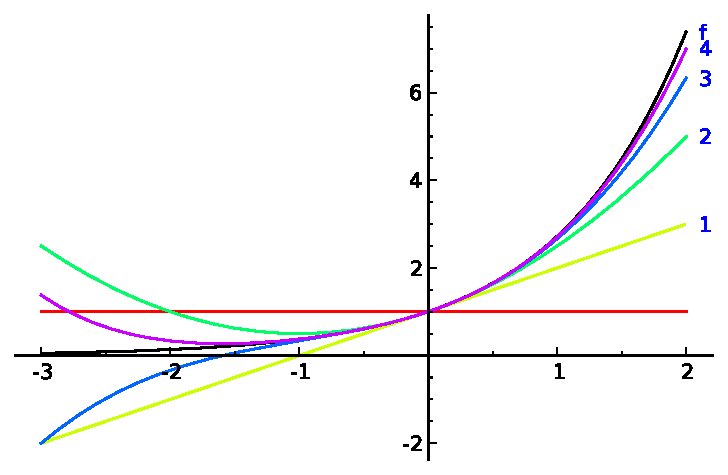
\includegraphics[width=\textwidth]{taylorexp.pdf}
 \end{center}

\subsubsection{Gegenbeispiel}
Die Funktion
\[ f(x) = \left \{ \begin{array}{ll}
\exp(-1/x^2), & \mbox{ für } x \neq 0\\
0, & \mbox{ für } x = 0\\
\end{array} \right. \]
ist nicht durch ihre Taylorreihe an $x_0=0$ darstellbar. Die Taylorreihe zu $f$
ist identisch $0$, da $f^{\,n}(0)=0$ ist für alle $n \in \mathbb{N}$. \\
\begin{sagein}
plot(exp(-1/x^2),(-0.5,0.5)) 
\end{sagein}
\begin{center}
  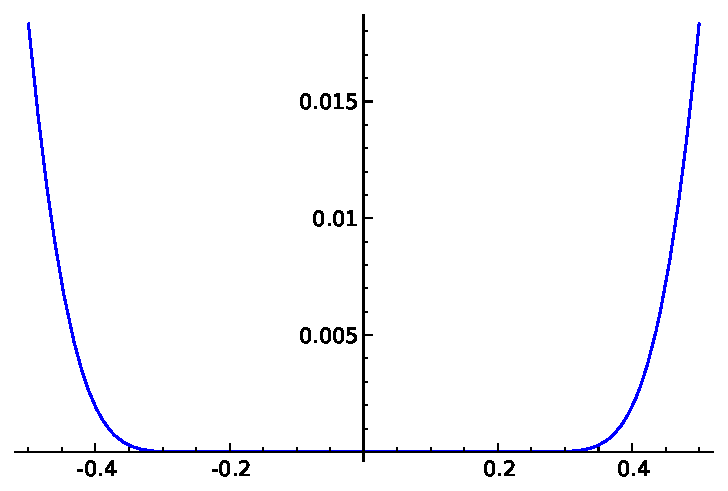
\includegraphics[height=4cm]{taylorgegen.pdf}
 \end{center}

\subsubsection{Die Taylorformel in Sage}
Natürlich ist für ein so nützliches Tool wie die Taylorentwicklung einer Funktion ein direkter Befehl in 
Sage vorhanden:
\begin{sagein}
taylor(f, x, x0, n)
\end{sagein}
Hierbei handelt es sich um das Taylorpolynom $(n-1)$-ten Grades zu einem Ausdruck $f$ 
(mit Unbekannten $x$) am Entwicklungspunkt $x0$. \\
Wir betrachten zwei kleine Beispiele:
\begin{sagein}
taylor(1/(1-x),x,0,5)
\end{sagein}
{\color{blue}\[ x^{5} + x^{4} + x^{3} + x^{2} + x + 1\]}
\begin{sagein}
taylor(sin(x),x,2,5)
\end{sagein}
{\small\color{blue}\[ \frac{1}{24} \, {\left(x - 2\right)}^{4} \sin\left(2\right) -
\frac{1}{6} \, {\left(x - 2\right)}^{3} \cos\left(2\right) - \frac{1}{2}
\, {\left(x - 2\right)}^{2} \sin\left(2\right) + {\left(x - 2\right)}
\cos\left(2\right) + \sin\left(2\right)\]}

%%%%%%%%%%%%%%%%%%%%%%%%%%%%%%%%%%%%%%
\section{Integration}
%%%%%%%%%%%%%%%%%%%%%%%%%%%%%%%%%%%%%%
Wir wollen uns dem Begriff des Integrals, wie üblich, durch Approximationen über Treppenfuktionen nähern. Hierfür 
brauchen wir einige Begriffe:
\begin{df}
Sei $[a,b]$ ein Intervall. Gilt $a=a_0 < a_1 <a_2 < \dots <
                                 a_n=b$, so nennt man $Z=(a_0, \dots
                                 ,a_n)$ eine Zerlegung von
                                 $[a,b]$.\\
Eine Funktion $\phi:[a,b] \rightarrow \mathbb{R}$ heißt 
                                 Treppenfunktion, wenn es eine
                                 Zerlegung $Z$ von $[a,b]$ gibt, so dass
                                 $\phi$ konstant ist auf jedem
                                 Teilintervall $(a_i,a_{i+1})$ von $Z$.\\
Wir erklären das Integral einer Treppenfunktion $\phi$ durch
\[\int_Z \phi := \sum_{k=1}^n c_k (a_k -a_{k-1}).\]
Dabei ist $Z$ die zugehörige Zerlegung und $c_k=\phi(x)$, $x\in
(a_{k-1},a_k)$.\\
Die Menge aller Treppenfunktionen auf $[a,b]$ sei $T[a,b]$.
Für eine beschränkte Funktion $f[a,b]\rightarrow \mathbb{R}$
heißt
\[ \int^*f:= \inf  \{ \int \psi \ | \ \psi \in T[a,b], f \leq \psi \}. \]
das Oberintegral und 
\[ \int_*f:= \sup  \{ \int \psi \ | \ \psi \in T[a,b], f \geq \psi \}.\]
das Unterintegral. Es gilt für $\phi, \psi \in T[a,b]$ mit
$\phi \leq f \leq \psi$ die Ungleichung
\[ \int \phi \leq \int_* f \leq \int^* f \leq \int \psi.\]
\end{df}
\subsubsection{Visualisierung in Sage}
Hier ein Plot, der die Funktionsweise der Approximation durch eine Treppenfunktion klärt:
\begin{sagein}
f = Piecewise([[(-pi,0),(cos(x)).function(x)]])
rsf = f.riemann_sum(10,mode="midpoint")
P = f.plot(rgbcolor=(0.7,0.1,0.5), plot_points=40)
Q = rsf.plot(rgbcolor=(0.7,0.6,0.6), plot_points=40)
L = add([line([[b,0],[b,f(x=b)]],rgbcolor=(0.7,0.6,0.6))+line([[a,0],[a,f(x=a)]],rgbcolor=(0.7,0.6,0.6)) for (a,b),f in rsf.list()])
(P + Q +L)
\end{sagein}
\begin{center}
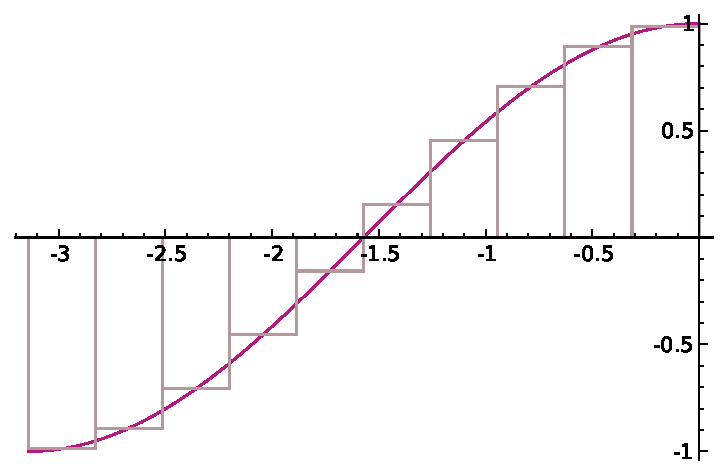
\includegraphics[width=6cm]{riemann.pdf}
\end{center}
\subsection{Das Riemann Integral}
Wir wollen das uns bekannte Riemannsche Integral formal definieren:
\begin{df}
Eine beschränkte Funktion $f:[a,b] \rightarrow \mathbb{R}$ heißt 
integrierbar, wenn Ober- und Unterintegral von $f$ auf $[a,b]$ übereinstimmen.\\
Der gemeinsame Wert heißt das Integral von $f$ und wird mit 
\[ \int_a^b f(x)dx \]
bezeichnet.\\ 
$f$ heißt der Integrand, $x$ die Integrationsvariable, $a$, $b$ sind die Integrationsgrenzen.
\end{df}
\subsubsection{Eigenschaften des Riemann Integrals}
Wir fassen einige grundlegende Eigenschaften des Riemann Integrals:\\
Das Integral ist linear, d.h.
\[ \int_a^b (\alpha f + \beta g) dx = \alpha \int_a^b fdx + \beta
\int_a^b g dx \]
Weiterhin ist es monoton, es gilt also:
\[  f \leq g \quad \Rightarrow \quad \int_a^b f dx \leq \int_a^b g
dx.\]
Sind $f,g$ integrierbar, so auch $f+g$, $f*g$, $f-g$,
$\max\{f,g\}$, $\min \{f,g \}$. 
Wir wollen einige wichtige Sätze über Integrale verstanden wissen.
\begin{sz}
Ist $f$ stetig auf einem Intervall $I$ und $a \in I$, so ist 
\[F(x)= \int_a^x f(t) dt, x \in I \] eine differenzierbare Funktion mit
$F\,'(x)=f(x)$. $F$ heißt Stammfunktion von $f$.\\
Eine alternative Notation für eine Stammfunktion $F$ ist  $\int f(x) dx$, das sog. unbestimmte Integral.\\
Ist $f$ stetig auf $[a,b]$, so gibt es ein $\xi \in [a,b]$ mit
\[\int_a^b f(x)dx = f(\xi) (b-a)\]
\end{sz}
\subsubsection{Integrale in Sage}
Um zu sehen, wie Sage mit Integralen umgeht, betrachten wir zuerst bestimmte Integrale der Form $\int_a^b f(x) dx$
\begin{sagein}
integrate(f,x,a,b) 
\end{sagein}
Dabei ist \isage{f} ein Ausdruck.Auch unbestimmte Integrale sind für Sage kein großes Problem:
\begin{sagein}
integrate(f,x)
\end{sagein}
Als dritte Möglichkeit der Integration steht uns die numerische Approximation zur Verfügung:
\begin{sagein}
numerical_integral(f,a,b) 
\end{sagein}
(benutzt die GSL-library).
Wir wollen uns diese Tatsachen an einigen Beispielen verdeutlichen:
\begin{sagein}
 integrate(sin(x),x,0,6)
\end{sagein}
\begin{sage}
-cos(6) + 1
\end{sage}
\begin{sagein}
integrate(exp(x)*x,x,2,3),integrate(exp(x)*x,x)
\end{sagein}
{\color{blue}\[\left(-e^{2} + 2 \, e^{3}, {\left(x - 1\right)} e^{x}\right)\]}
% \begin{sage}
% -e^2 + 2*e^3
% \end{sage}
\begin{sagein}
integrate(1/x^2,x,1,oo)
\end{sagein}
\begin{sage}
  1
\end{sage}
\begin{sagein}
numerical_integral(sin(1/x)*x,1,2)
\end{sagein}
\begin{sage}
  (0.91905916759870254, 1.0203606488609102e-14)
\end{sage}
\begin{sagein}
assume(a<>-1)
integrate(x^a*b,x)
\end{sagein}
{\color{blue} \[ \frac{b x^{{\left(a + 1\right)}}}{a + 1}\]}
% \begin{sage}
% b*x^(a + 1)/(a + 1)
% \end{sage}
\begin{sagein}
forget();a=-1
integrate(x^a*b,x)
\end{sagein}
{\color{blue} \[ b \log\left(x\right)\]}
% \begin{sage}
%  b*log(x)
% \end{sage}
\subsubsection{Uneigentliche Integrale}
Wir wollen den Begriff des uneigentlichen Integrals einführen:
\begin{df}
Sei $f$ auf $[a,b)$ erklärt (eventuell $b=\infty$) und sei $f$ auf jedem
abgeschlossenen Teilintervall integrierbar. Man definiert
\[  \int_a^b f(x)dx := \lim_{z \rightarrow b (-0)} \int_a^z f(x)dx,\]
falls der Limes existiert. Man spricht von einem 
uneigentlichen Integral.
\end{df}
\subsubsection{Funktionenfolgen}
Wir wollen hier noch zwei kleine Aussagen über Funktionenfolgen bzgl. Integration bzw. Differentiation platzieren:
\begin{sz}
Sei $(f_n)_n$ eine Folge integrierbarer Funktionen auf
$[a,b]$. Konvergiert $(f_n)_n$ gleichmäßig, so ist die Grenzfunktion
integrierbar mit
\[ \int_a^b \lim_{n \rightarrow \infty} f_n(x) dx = \lim_{n
\rightarrow \infty} \int_a^b f_n(x) dx .\]
 Sei $(f_n)_n$ eine Folge differenzierbarer Funktionen auf
$[a,b]$. $(f\,'_n)_n$ konvergiere gleichmäßig und es existiere ein $x_0
\in [a,b]$ für das $f_n(x_0)$ konvergiert. Dann konvergiert $(f_n)_n$
gleichmäßig mit $( \lim_{n \rightarrow \infty} f_n(x))' = \lim_{n
\rightarrow \infty} f\,'_n(x)$.  
\end{sz}

%%%%%%%%%%%%%%%%%%%%%%%%%%%%%%%%%%%%%%
\chapter{Sage Werkzeugkasten}
\section{Interaktion}
\subsection{Umgang mit Strings}
%%%%%%%%%%%%%%%%%%%%%%%%%%%%%%%%%%%%%%
Wir wollen uns hier mit Zeichenketten (engl. strings) befassen. Dabei handelt es sich um eine geordnete
Aneinanderreihung von Zeichen. Zeichen sind z.B. Buchstaben, Ziffern,
Sonderzeichen,... Mit ihnen kann man in Sage Texte gestalten. Sie sind wichtig
für die Ausgabe der Ergebnisse. Ihr Datentyp ist \isage{str} und sie werden in Hochkommas oder Anführungszeichen 
eingeschlossen. Wir betrachten einige Beispiele:
\begin{sagein}
text1 = 'Dies ist ein String.'; text1
\end{sagein}
\begin{sage}
'Dies ist ein String.'
\end{sage}
\begin{sagein}
text2 = "Dies ist noch ein String."; text2
\end{sagein}
\begin{sage}
'Dies ist noch ein String.'
\end{sage}
\begin{sagein}
type(text1)
\end{sagein}
\begin{sage}
<type 'str'>
\end{sage}
\subsubsection{Zugriff}
Der Zugriff auf Strings gestaltet sich so, wie wir das schon gewohnt sind, über den Index:
\begin{sagein}
text1[0], text1[3], text1[2:4], text1[0:4:2]
\end{sagein}
\begin{sage}
('D', 's', 'es', 'De')
\end{sage}
Wir können leicht Ersetzungen innerhalb eines Strings vornehmen:
\begin{sagein}
text1.replace('Dies','Das')
\end{sagein}
\begin{sage}
'Das ist ein String.'
\end{sage}
\subsubsection{Operationen auf Strings}
Wir betrachten weitere Operationen auf Strings, zuerst das Zusammenhängen von solchen:
\begin{sagein}
A='Letzte '; B='Vorlesung'; A+B
\end{sagein}
\begin{sage}
'Letzte Vorlesung'
\end{sage}
 \isage{len()} gibt die Anzahl der Zeichen in einer Zeichenkette
an:
\begin{sagein}
a=len(A+B); a
\end{sagein}
\begin{sage}
  16
\end{sage}
Wir können durch geschickte Indexwahl Zugriffe beginnend vom Ende vornehmen:
\begin{sagein}
(A+B)[-1]
\end{sagein}
\begin{sage}
  'g'
\end{sage}
 {\color{blue} \isage{str()}} wandelt Objekte in einen String um:
\begin{sagein}
str(x^2+2), str([1,2,3])
\end{sagein}
\begin{sage}
('x^2 + 2', '[1, 2, 3]')
\end{sage}
Mittels {\color{blue} \isage{find()}} können wir Strings in Strings suchen:
\begin{sagein}
'Hallo'.find('lo')
\end{sagein}
\begin{sage}
3
\end{sage}
 \begin{sagein}
'Hallo'.find('gnu')
\end{sagein}
\begin{sage}
-1
\end{sage}
\begin{bem}
 \isage{find()} liefert offensichtlich den Index zurück, an der der gesuchte String steht oder $-1$, falls der String nicht 
enthalten ist.
\end{bem}
Durch {\color{blue} \isage{split()}} können wir Strings aufspalten:
\begin{sagein}
text = 'Dies ist ein Satz, und ein Nebensatz'
text.split() 
\end{sagein}
\begin{sage}
 ['Dies', 'ist', 'ein', 'Satz,', 'und', 'ein', 'Nebensatz']
\end{sage}
\begin{sagein}
text.split('i')
\end{sagein}
\begin{sage}
['D', 'es ', 'st e', 'n Satz, und e', 'n Nebensatz']
\end{sage}
\subsubsection{Formate und print}
Nachdem wir nun Strings kennen und diese manipulieren können, 
müssen wir noch wissen, wie genau wir Strings ausgeben können. 
Dies geschieht via
\begin{sagein}
  print 'Text %<format> und %<format> ... ' % (x,y,...)
 \end{sagein}
dabei sind für \isage{<format>} folgende Optionen möglich:
\begin{sagein}
%[<flag>][<minwidth>][.<precision>]converter 
\end{sagein}
Für die einzelnen Optionen gilt:
\begin{itemize}
\item \isage{flag}: 0 für das Auffüllen mit Nullen
\item \isage{minwidth}: Minimale Breite der Darstellung
\item \isage{precision}: Genauigkeit (Nachkommastellen)
\item \isage{converter}:\\
\begin{tabular}{cp{10cm}}
\isage{'i'} & ganze Zahl mit Vorzeichen\\
\isage{'e'} & Gleitkommazahl mit Exponentialformat (kleingeschrieben).\\
\isage{'f'} &Gleitkommazahl im Dezimalformat.\\
\isage{'g'} &Gleitkommazahl. Benutzt kleingeschriebene Exponentialform, wenn der Exponent kleiner als -4 oder der Genauigkeit ist, ansonsten Dezimalformat.
\end{tabular}
\end{itemize}
Wir betrachten einige Beispiele:
\begin{sagein}
print '%5s | %7s' % ('Index','Wert')
for k in srange(1,25,9.55): 
    print '%5i | %07.3f' % (k,k^2) 
\end{sagein}
\begin{sage}
Index |    Wert
    1 | 001.000
   10 | 111.303
   20 | 404.010
\end{sage}
\subsubsection{Interaktive Plots}
Wir wollen hier an einem Beispiel den interaktiven Plot vorstellen:
\begin{sagein}
@interact
def _(b = range_slider(-20, 20, 1, default=(-19,3), label='Range')):
    plot(sin(x)/x, b[0], b[1]).show(xmin=b[0],xmax=b[1]) 
\end{sagein}
\begin{center}
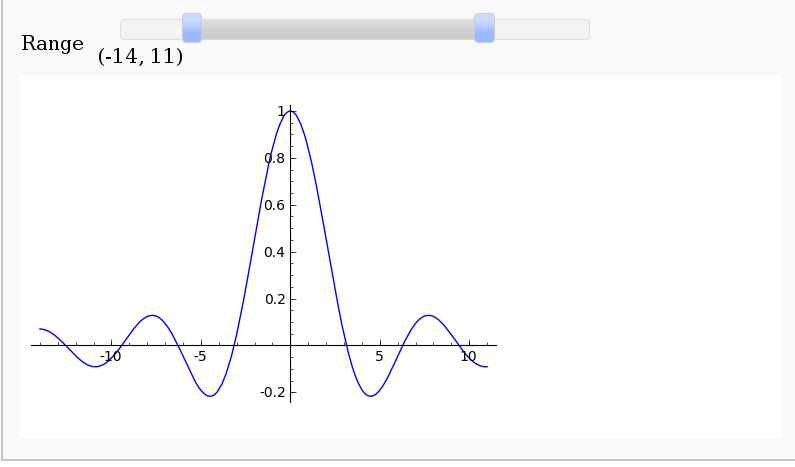
\includegraphics[width=0.8\textwidth]{interact_basis.png}
\end{center}
\subsubsection{Der Regler}
Wir spezifizieren hier die Erstellung des Reglers.\\
Wir erhalten einen Regler mit Werten von vmin bis vmax durch:
\begin{sagein}
u=slider(vmin, vmax=, step_size=1, default=, label=) 
\end{sagein}
Ein Regler eines Intervalles wird erzeugt mit:
\begin{sagein}
u=range_slider(vmin, vmax=, step_size=1, default=, label=)
\end{sagein}
Wir können auch ein Ankreuzfeld erstellen:
\begin{sagein}
u=checkbox(default=True, label=)
\end{sagein}
Auch ein Aufklappmenü (oder Knöpfe, wenn nrows, ncols, oder buttons gesetzt ist) ist 
problemlos darstellbar:
\begin{sagein}
u=selector(values, label=, nrows=, ncols=, buttons=False)
\end{sagein}
Sogar Textblöcke können dargestellt werden:
\begin{sagein}
u=text_control(value='')
\end{sagein}
\subsubsection{Interaktive Taylorentwicklung}
Wir betrachten unsere neue Errungenschaft am Beispiel der Taylorentwicklung:
\begin{sagein}
var('x')
x0  = 0
f   = sin(x)*e^(-x)
p   = plot(f,-1,5, thickness=2)
dot = point((x0,f(x=x0)),pointsize=80,rgbcolor=(1,0,0))
@interact
def tayl(order=slider(1,12,1,label='order')):
    ft = f.taylor(x,x0,order)
    pt = plot(ft,-1, 5, color='green', thickness=2)
    print ('f(x) = %s'% f)
    print ('f^(x;%s) = %s + O(x^(%s))'%(x0,ft,order+1))
    show(dot + p + pt, ymin = -.5, ymax = 1)
\end{sagein}
\begin{center}
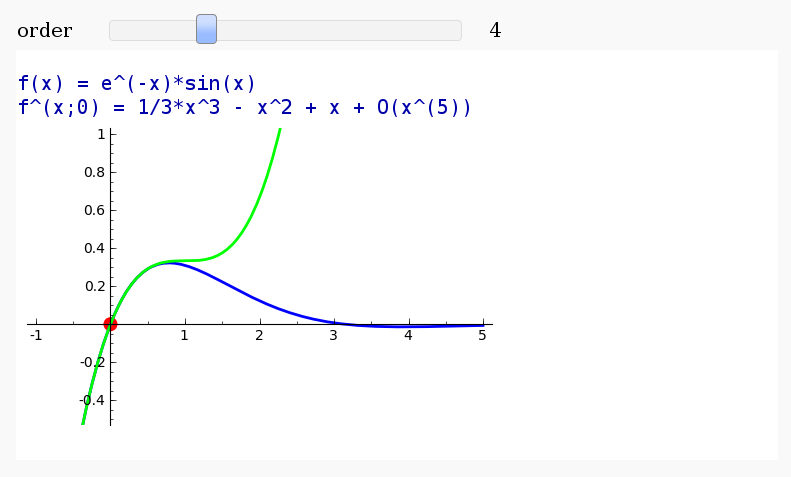
\includegraphics[width=\textwidth]{interact1.png}
\end{center}
\subsubsection{Grafiken einer Abstandsfunktion}
Als weiteres Beispiel des interaktiven PLots betrachten wir eine Abstandsfunktion:
\begin{sagein}
@interact
def _(q1=slider(-3,3,default=-1), q2=slider(-3,3,default=-2), cmap=selector(['autumn', 'bone', 'cool', 'copper', 'gray', 'hot', 'hsv','jet', 'pink', 'prism', 'spring', 'summer','winter'])):
     x,y = var('x,y')
     f = q1/sqrt((x+1)^2 + y^2) + q2/sqrt((x-1)^2+(y+0.5)^2)
     C = contour_plot(f, (x,-2,2), (y,-2,2), plot_points=30, contours=15, cmap=cmap)
     show(C, figsize=3, aspect_ratio=1)
     show(plot3d(f, (x,-2,2), (y,-2,2)), figsize=5, viewer='tachyon')
\end{sagein}
\begin{center}
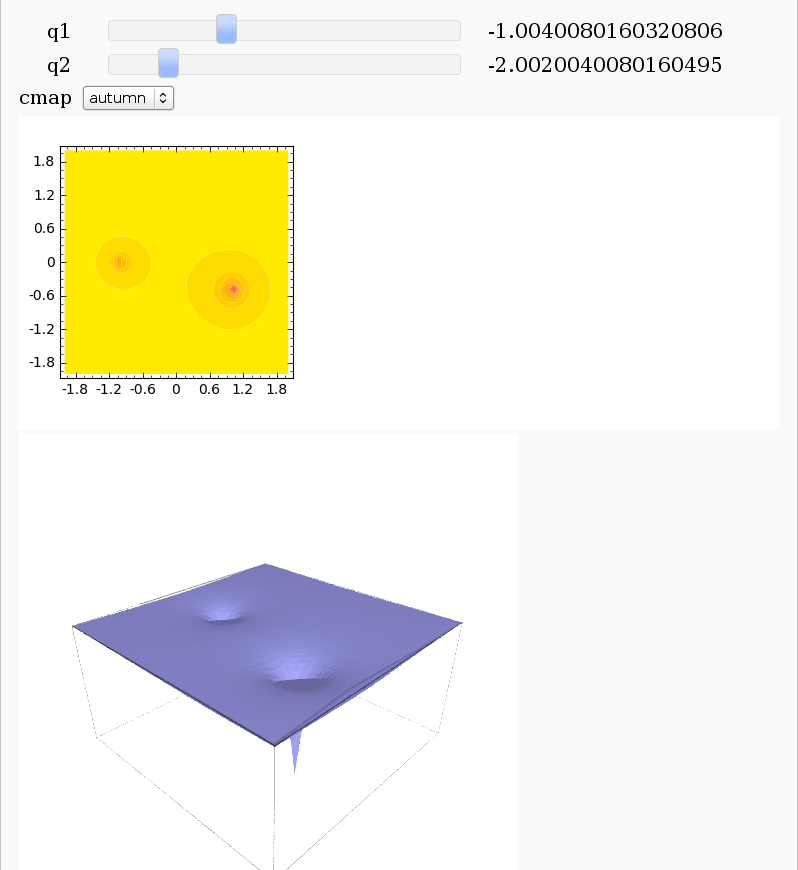
\includegraphics[width=7.5cm]{interact2.png}
\end{center}
\subsubsection{GeoGebra}
In Sage lassen sich GeoGebra Objekte einbetten. Das funktioniert wie folgt:
\begin{itemize}
 \item  In GeoGebra: Erstellen eines Objektes
 \item  In GeoGebra: File> Export> Dynamic worksheet.
 \item  In Sage notebook: Data> Die .jar (von GeoGebra) und die .ggb hochladen.
 \item  Aus dem Exportierten .html den Teil mit <applet> kopieren und im worksheet in Sage unter Edit kopieren( Edit> Paste ).
 \item  Im Editier-tab die codebase zu "./data/" ändern
 \item  Fertig!
\end{itemize}

\begin{center}
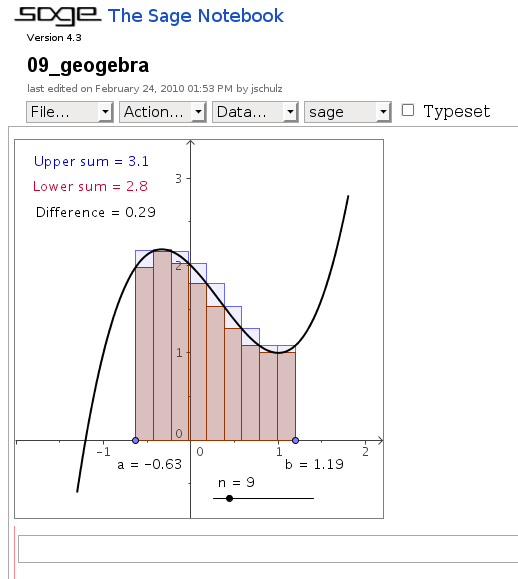
\includegraphics[width=0.6\textwidth]{geogebra.png}
\end{center}

%%%%%%%%%%%%%%%%%%%%%%%%%%%%%%%%%%%%%%
\section{Beispiele Programmierung}
%%%%%%%%%%%%%%%%%%%%%%%%%%%%%%%%%%%%%%
Wir wollen uns hier noch ein wenig der Programmierung in Sage hingeben. Dazu implementieren wir 
einige zum Teil bekannte Algorithmen.
\subsubsection{Größter gemeinsamer Teiler}
Wir wollen die
Berechnung des ggT von natürlichen Zahlen $a$ und $b$ mit Hilfe des
euklidischen Algorithmus implementieren. Dazu verfolgen wir folgende Idee:
\begin{enumerate}
\item  $ggT(a,b)=ggT(a,b-a)$ für $a<b$.
\item $ggT(a,b)=ggT(b,a)$.
\item $ggT(a,a)=a$.
\end{enumerate}
Daraus erhalten wir folgendes Algorithmus:\\
Wiederhole,  bis $a=b$
\begin{itemize} 
\item Ist $a>b$, so $a=a-b$.
\item Ist $a<b$, so $b=b-a$ 
\end{itemize}
In Sage erhalten wir also:
\begin{sagein}
def ggT(a,b):  
    """Bestimme den ggT von a und b"""
    while a<>b:
        if a>b:
            a = a-b
        else: 
            b = b-a
    return a
ggT(6,9)
\end{sagein}
\begin{sage}
3  
\end{sage}
\subsubsection{Primzahlzwillinge}
Ein weitere interessanter Algorithmus ergibt sich, wenn man versucht, Primzahlzwillinge zu berechnen:
\begin{sagein}
T = []; anz = 0
for i in [2..100]:
    if (is_prime(i) and is_prime(i+2)):
        anz += 1
        T.append([i,i+2])
print('Anzahl = %s' % anz);T
\end{sagein}
\begin{sage}
Anzahl = 8
[[3, 5], [5, 7], [11, 13], [17, 19], [29, 31], [41, 43], [59, 61], [71,
73]]
\end{sage}
\subsubsection{Betrag}
Wir möchten den Betrag (auch komplexer Zahlen!!!) berechnen. Unser Algorithmus sieht so aus:
\begin{sagein}
def betrag(a):
    if a in ZZ or a in QQ or a in RR:
        if a>0:
            y = a
        else:
            y = -a
    elif a in CC:
        y = sqrt(real(a)^2+imag(a)^2)
    else:
        return 'Falscher Eingabetyp'
    return y
betrag([1,2]), betrag(2+I*2)
\end{sagein}
\begin{sage}
('Falscher Eingabetyp', 2*sqrt(2))
\end{sage}
\subsubsection{Gültigkeit von Variablen}
Im Zusammenhang mit Programmierung muss man über den Güligkeitsbereich von Variablen sprechen. Mit der 
Gültigkeit von Variablen ist die Bestandsdauer von Variablen bzw. der Werte dieser Variablen gemeint. 
Man unterscheidet hier globale und lokale Variablen:
\begin{df}
Im aktuellen Worksheet sind alle Variablen/Funktionen global, 
d.h. die den Variablen zugewiesenen Werte bleiben für die
gesamte Laufzeit vom jeweiligen worksheet erhalten, bis sie geändert werden. 
Man kann auf die Variablen jederzeit zugreifen und die Werte der Variablen
ändern.\\
Lokale Variablen sind nur innerhalb einer Prozedur/Funktion 
gültig. Nach Beenden der Prozedur werden
diese Variablen wieder gelöscht. 
\end{df}
\subsubsection{Mandelbrotmengen}
Wir wollen Mandelbrotmengen betrachten. Die Mandelbrot-Menge ist die Menge von Punkten $c \in \mathbb{C}$
bei denen die Folge $(z_n)_n$, die durch
\[ z_0:=c, \qquad  z_{n+1} = z_n^2 +c, \quad n \in \mathbb{N}\]
definiert ist, beschränkt ist. Als Algorithmus erhalten wir:
\begin{sagein}
def mandel(x,y):
    c = (x + I*y).n()
    z = c
    it = 0
    max_it = 150
    while abs(z)<2 and it<max_it:
        z = z^2 + c
        it += 1
    return float(it/max_it)
\end{sagein}
Die Funktion \isage{mandel} gibt zu $x+iy$ die relative Anzahl der
Iterationsschritte zurück. Der Plot einer solchen Mandelbrotmenge hat dann diese Gestalt:
\begin{sagein}
density_plot(mandel, (-2.1,1.2), (-1.1,1.1), plot_points=100)
\end{sagein}
\begin{center}
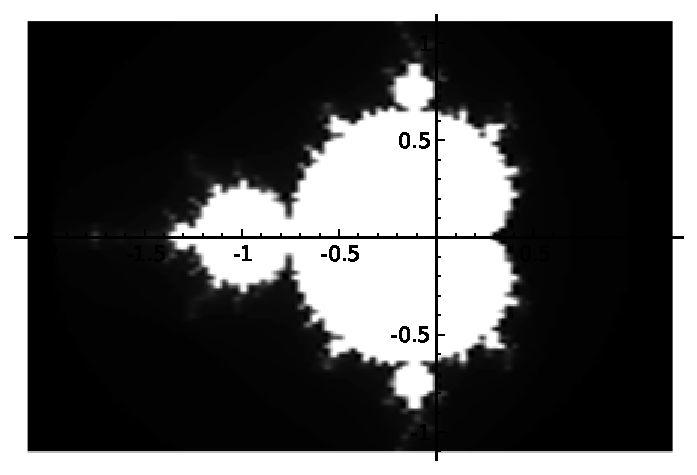
\includegraphics[width=0.8\textwidth]{mandel.pdf} 
\end{center}
\subsubsection{Programmierparadigmen}
Wir müssen im Zuge der Programmierung auch auf gewisse Programmierregeln eingehen. Einige der Wichtigsten sind:
\begin{itemize}
\item Hilfetext: Ein Programm sollte im Hilfetext eine gute Beschreibung der Funktionsweise der Funktion enthalten. Dieser sollte insbesondere Ein- und Ausgabe-Variablen genau beschreiben.
\item Kommentieren: Im Programm sollte durch Kommentare dokumentiert werden, was einzelne, wesentliche Abschnitte/Zeilen im Programm tun.
\item Passende Benennung von Variablen/Funktionen: Variablen und Funktionen sollten durchdacht benannt werden, d.h. man sollte an ihnen im Optimum direkt erkennen können, welchem Zweck sie im gegebenen Kontext dienen. 
\end{itemize}
\subsubsection{g-adische Darstellung}
Wir wollen die g-adische Darstellung einer natürlichen Zahl programmieren:
\begin{sagein}
def Gadisch(x,basis):
    """Berechnung der Darstellung einer natuerlichen Zahl 
x zur Basis b. Rueckgabe des Ergebnis als Liste!"""
    #Abfangen der Eingabe
    if not x in ZZ or x < 0 or basis==1: 
        return 'Eingabe nicht korrekt!'
    T = []  # leere Liste 
    while x>0:
        T.append(x%basis) # Rest der Division
        print '%i : %i = %i Rest %i' % (x,basis,floor(x/basis),x%basis)
        x = floor(x/basis) # Teiler setzen
    # Rueckgabe der Liste
    return T
\end{sagein}

\begin{sagein}
Gadisch(6,2)
\end{sagein}
\begin{sage}
6 : 2 = 3 Rest 0
3 : 2 = 1 Rest 1
1 : 2 = 0 Rest 1
[0, 1, 1]
\end{sage}

\begin{sagein}
Gadisch(3.4,2)
\end{sagein}
\begin{sage}
'Eingabe nicht korrekt!'
\end{sage}
\subsubsection{Kochsche Kurve}
Seien $y_1,y_2$ zwei Punkte im $\mathbb{R}^2$. Betrachte die Strecke mit Endpunkten $y_1$ und $y_2$. 
Ersetze  diese Strecke durch 4 Strecken 
$\overline{y_1 z_1}$, $\overline{z_1 z_2}$, $\overline{z_2 z_3}$,
$\overline{z_3 y_2}$ mit Endpunkten 
\begin{eqnarray*}
 z_1 &=&\frac23 y_1 + \frac13 y_2\\[0.5cm]
 z_2 &=& \frac{\sqrt{3}}{6} \left( \begin{array}{cc}
 0 & 1 \\ -1 & 0 \\
 \end{array} \right)
 (y_1 - y_2) + \frac12 (y_1 + y_2)\\[0.5cm]
 z_3 &=&\frac13 y_1 + \frac23 y_2
\end{eqnarray*}
 Dieses Prozedere wird nun für jede einzelne Teilstrecke wiederholt.
\begin{sagein}
def koch(y1,y2,lev):
    Listelinien = []
    if (lev == 0):
        Listelinien.append(line([(y1[0],y1[1]),(y2[0],y2[1])]))
    else:
        # Definieren der neuen Punkte 
        z1 = 2/3 * y1 + 1/3 * y2
        z3 = 1/3 * y1 + 2/3 * y2
        z2 = sqrt(3)/6*matrix([[0, 1],[ -1, 0]])*(y1-y2) + 1/2 * (y1 + y2)
        # Definieren der 4 Strecken
        Listelinien.append(koch(y1, z1, lev-1))
        Listelinien.append(koch(z1, z2, lev-1))
        Listelinien.append(koch(z2, z3, lev-1))
        Listelinien.append(koch(z3, y2, lev-1))
    return add(Listelinien)
\end{sagein}

\begin{sagein}
# Einfacher Fall einer Linie 
koch(vector([0,0]),vector([1,0]),4)
\end{sagein}
\begin{center}
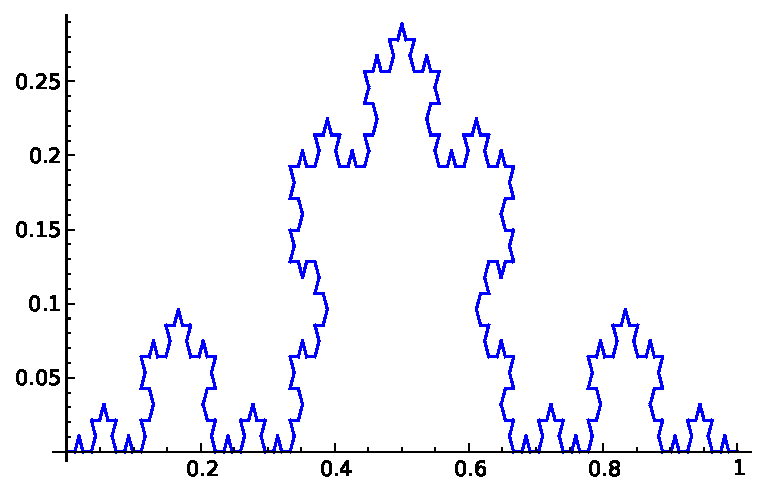
\includegraphics[width=0.7\textwidth]{koch.pdf} 
\end{center}
\end{document}